



%----------------------------------------------------------------------------------------

\newpage

%\section[Interaction model][Modèle d'interaction]{Dynamical extension of the interaction model}{Extension dynamique du modèle d'interaction}
\section{Dynamical extension of the interaction model}{Extension dynamique du modèle d'interaction}



\label{sec:macrocoevol}



%----------------------------------------------------------------------------------------


Nous pouvons à présent faire la synthèse d'une part des paradigmes d'intégration d'un système de ville et du réseau de transport, effectué de manière statique pour le comportement du réseau dans le modèle d'interaction développé et exploré en section~\ref{sec:interactiongibrat}, d'autre part des indicateurs pour la compréhension d'un modèle de co-évolution pour un système de villes,\comment[FL]{reprendre tous ces concepts : modele, indicateur etc sont ici trop mis au meme niveau} expérimentés dans la section précédente~\ref{sec:macrocoevolexplo}, ainsi que de manière indicative pour comparaison des comportements obtenus pour le modèle SimpopNet. Cette synthèse consiste en une première formulation d'un \emph{modèle de co-évolution macroscopique pour les systèmes de villes}, qui est un élément clé pour apporter un éclaircissement partiel de notre problématique générale.\comment[FL]{oui !}

\comment[AB]{reformuler}


%%%%%%%%%%%%%%%%%
\subsection{Macroscopic Model of Co-evolution}{Modèle macroscopique de co-évolution}


%%%%%%%%%%%%%%%%%
\subsubsection{Rationale}{Hypothèses et choix de modélisation}



\bpar{
In a multi-modeling fashion, the model can take into account various processes such as between cities direct interactions, network-mediated interactions, feedback of network flows, and for the network demand-induced growth.
}{
Cette première approche se place dans une logique d'extension directe du modèle d'interactions au sein d'un système de villes présenté en chapitre~\ref{ch:evolutiveurban}, c'est à dire à une échelle macroscopique et avec une ontologie typique aux systèmes de villes. Toujours dans un choix de simplicité%, dont la relaxation pourra être explorée pour le cas d'application à la Chine avec l'ajout de variables économiques
, nous restons ici\comment[AB]{{\_}} à une description unidimensionnelle des villes par leur population. Concernant la croissance du réseau, nous proposons de nous placer également à un niveau relativement agrégé et simplifié, en permettant de tester des heuristiques de croissance à différents niveaux d'abstraction. Dans une logique de multi-modélisation,\comment[FL]{sens ?} le modèle peut prendre en compte divers processus comme les interactions directes entre les villes, les interactions intermédiaires par le réseau, la rétroaction des flux de réseau et une croissance du réseau induite par la demande. Les éléments empiriques mis en valeur pour le réseau ferré français par~\cite{thevenin2013mapping} suggèrent l'existence de retroactions de l'utilisation du réseau, ou des flux le traversant, sur sa persistence et son développement, dont les propriétés ont évolué dans le temps : une première phase de développement fort correspondrait à une réponse à des demandes\comment[FL]{?} même faibles, tandis que le renforcement des liens principaux et la disparition des liens faibles observés plus tard s'interpréterait comme une rétroaction dont le signe est fixé par seuil.\comment[AB]{?}\comment[AB]{pas super clair}
}





%%%%%%%%%%%%%%%%%
\subsubsection{General Formulation}{Formulation Générique}



%%%%%%%%%%%%%%%%%
\begin{figure}
\includegraphics[width=\linewidth]{Figures/MacroCoEvol/model}
\caption[Schematic Model Representation][Schématisation du modèle]{}{\textbf{Représentation abstraite du modèle.} Les ovales correspondent aux éléments ontologiques principaux (Villes, Réseau, Flux), tandis que les flèches traduisent des processus et les paramètres associés. Le modèle est décrit dans son écosystème plus large d'initialisation et d'indicateurs de sortie.\comment[AB]{couplage indirect villes/reseaux via les flux ?}\comment[FL]{donc tu as choisi l'echelle interurbaine ici, il faut absolument que ca ressorte clairement}\label{fig:macrocoevol:model}}
\end{figure}
%%%%%%%%%%%%%%%%%


Le système urbain est caractérisé par les populations $\mu_i(t)$ et le réseau $\mathbf{N}(t)$\comment[AB]{pas terrible, p 272 N = effectif, ce qui est plus logique} auquel on peut associer une matrice de distance $d^N_{ij}(t)$. Les flux entre villes $\phi_{ij}$ suivent les expressions données en~\ref{sec:interactiongibrat} avec la distance réseau. De la même manière, la variation des populations suit les spécifications du modèle de base. La Fig.~\ref{fig:macrocoevol:model} exprime le modèle sous forme schématisée.




\paragraph{Network Growth}{Croissance du réseau}


Concernant le réseau, en toute généralité\comment[FL]{non c'est deja un choix} celui-ci évolue suivant $\mathbf{N}(t + 1) = F(\mathbf{N}(t),\phi_{ij}(t))$, de telle façon qu'une assignation des flux dans le réseau ainsi qu'un variation locale de ses éléments est possible. Nous proposons dans un premier temps de nous intéresser aux motifs liés à la distance uniquement, et de spécifier une relation sur un réseau abstrait uniquement par $d^N_{ij}(t+1) = F(d^N_{ij}(t),\phi_{ij}(t))$.\comment[FL]{la difference entre les deux formules est subtiles, expliciter} Dans cette logique, nous restons dans un modèle d'interaction à l'echelle macroscopique uniquement (puisqu'un spatialisation précise du réseau implique la prise en compte d'une échelle plus fine).\comment[AB]{developper}

Suivant l'heuristique de rétroaction par seuil, étant donné un flux $\phi$ dans un lien, on suppose que sa distance effective est mise à jour par :

\[
d(t+1) = d(t)\cdot \left( 1 + g_{max} \cdot \left[\frac{1 - \left(\frac{\phi}{\phi_0}\right)^{\gamma_s}}{1 + \left(\frac{\phi}{\phi_0}\right)^{\gamma_s}}\right]\right)
\]

\comment[AB]{donner une intuition + references}

cf Tero ? papier Francois \cite{2013arXiv1301.6628K}
% implementation
% https://github.com/fqueyroi/tulip_plugins/tree/master/TransportationNetworks



avec $\gamma_s$ un paramètre de hiérarchie, $\phi_0$ le paramètre de seuil et $g_{max}$ le taux de croissance maximal qui peut s'ajuster à des valeurs réalistes par exemple par l'intermédiaire du calcul de $(1+g_{max})^{t_f}$.\comment[FL]{phrase tres floue}




\subsubsection{Implementation}{Implémentation}



\bpar{
}{
Le couplage du modèle d'interaction à la prise en compte\comment[AB]{pas clair} plus fine des processus de réseau rend plus difficile l'intégration complète dans un plugin OpenMole comme c'était le cas pour le modèle étudié en~\ref{sec:interactiongibrat}.\comment[AB]{preciser} L'utilisation d'un workflow comme médiateur pour le couplage est une solution intéressante mais réaliste uniquement dans le cas d'un couplage faible. L'un des défis que devra relever la bibliothèque de méta-modélisation en cours de développement autour d'OpenMole, serait la possibilité de coupler fortement (par exemple au sens de dynamiquement dans l'évolution de la simulation) des composantes hétérogènes de manière transparente.\comment[AB]{pourquoi ? $\rightarrow$ preciser} Nous optons pour ce modèle pour une implémentation complète en NetLogo pour une simplicité de couplage des composantes. Une attention particulière est portée à la dualité de la représentation du réseau, à la fois sous forme de matrice de distance et sous forme physique, pour permettre facilement l'extension à des heuristiques de réseau physique.\comment[FL]{mal mis en valeur}
}






%%%%%%%%%%%%%%%%%
\subsection{Application to Synthetic Data}{Application à des Données Synthétiques}


\bpar{
The model is first tested and explored on synthetic city systems, generated following a simple heuristic to follow the rank-size law and Central Place Theory.
%The systematic exploration through intensive computation unveils different interaction regimes across the parameter space. In some, the introduction of the network can drastically change the fate of some cities, whereas the top-distribution hierarchy is reinforced, what is consistent with empirical observations in the literature. Some regimes suggest circular causalities between network and city growth, corresponding to the co-evolution.
}{
Le modèle est d'abord testé et exploré sur des systèmes de villes synthétiques, afin de comprendre certaines de ses propriétés intrinsèques. Dans ce cas, nous considérons le modèle avec réseau abstrait comme spécifié ci-dessus, c'est à dire sans explicitation spatiale du réseau et avec les règles d'évolution agissant directement sur $d^N_{ij}$ selon les spécifications données précédemment.
}


\paragraph{Synthetic data}{Données Synthétiques}

\comment[FL]{la plus simple possible ? non le plus simple possible cest une ville de taille 1 au milieu (mais cest un point de vue)}

Un système de villes synthétiques est généré, en suivant l'heuristique utilisée dans la section précédente : (i) des villes en nombre $N_S$ sont placées aléatoirement dans le plan euclidien; (ii) les populations sont attribuées aux villes selon une loi de puissance inverse, avec un paramètre de hiérarchie $\alpha_S$ et de telle façon que la plus grande ville ait une population $P_{max}$, c'est-à-dire suivant $P_i = P_{max} \cdot i^{-\alpha_S}$. Pour simplifier\comment[FL]{reprendre formulation : comment simplifier ce qui est deja le plus simple possible ?}, le nombre de villes est fixé à $N_S = 30$, la population maximale à $P_{max} = 100000$ et la croissance maximale du réseau à $g_{max} = 0.005$. Le temps final est fixé à $t_f = 30$, ce qui correspond à des distances divisées par 5 environ (puisque $(1 - 0.05)^{30} \simeq 0.214$)\comment[FL]{suppr}, en cohérence \comment[FL]{surtout cetait un critere j'imagine}avec un passage du Paris-Lyon en une dizaine d'heures au début du 19ème siècle à deux heures aujourd'hui. Nous négligeons aussi les effets de réseau au second ordre en fixant $w_N = 0$.


\paragraph{Results}{Résultats}

%%%%%%%%%%
% -- ON HOLD
% sensibilite a \alpha_S 


Nous explorons une grille de l'espace des paramètres $(\alpha_S,\phi_0,\gamma_s,w_G,d_G,\gamma_G)$. Nous utilisons les indicateurs introduits en~\ref{sec:macrocoevolexplo} pour quantifier le comportement du modèle dans l'espace des paramètres. En Fig.~\ref{fig:macrocoevol:behavior}, nous montrons l'évolution d'indicateurs dans le temps ainsi que des mesures agrégées, pour une grande partie de l'espace des paramètres couvert. Nous montrons les résultats pour $\alpha_S = 1$, valeur la plus proche d'un système de villes réel\comment[FL]{preuve de cette affirmation ?}[cit Clem Metazipf]. L'évolution de la centralité de proximité moyenne dans le temps, visualisée pour $w_G = 0.001$, et à $(d_G,\gamma_G,\phi_0)$ variables, témoigne d'une transition en fonction du niveau de hiérarchie : lorsque celui-ci décroit, on observe l'émergence de trajectoires où la centralité moyenne croît dans le temps, ce qui correspond à des situations où l'ensemble des villes bénéficie d'accroissements d'accessibilité.\comment[AB]{preciser les graphiques dont tu parles !} En terme d'entropie des populations, l'ensemble des paramètres donne une entropie décroissante, c'est à dire des convergences des trajectoires dans le temps\comment[FL]{c'est vite dit, tu sembles mettre tous les parametres au meme niveau}.\comment[JR]{note de bas de page lien entropie et convergence} Lorsqu'on s'intéresse à la complexité des trajectoires d'accessibilité, on note pour des valeurs de $\phi_0 > 1.5$ un maximum de la complexité en fonction de la distance d'interaction $d_G$, stable lorsque $w_G$ et $\gamma_G$ varient. Cette échelle intermédiaire peut être interprétée comme produisant des sous-systèmes régionaux, assez grands pour développer chacun un certain niveau de complexité, et assez isolés pour ne pas uniformiser les trajectoires sur l'ensemble de l'espace. Nous reconstruisons ainsi une non-stationnarité spatiale, typiquement observée en~\ref{sec:staticcorrelations}, et rejoignons le concept de niche écologique localisée dans l'espace (voir~\ref{sec:theory}).\comment[AB]{developper} Enfin, le comportement des corrélations de rang pour l'accessibilité révèle que la distance d'interaction augmente systématiquement le nombre d'inversions de hiérarchie, ce qui correspond en un sens à une augmentation de la complexité globale du système. Le paramètre de hiérarchie diminue quant à lui cette corrélation, ce qui veut dire qu'une évolution plus hiérarchique affectera un plus grand nombre de villes dans l'aspect qualitatif de leur trajectoires.



%%%%%%%%%%%%%
\begin{figure}
%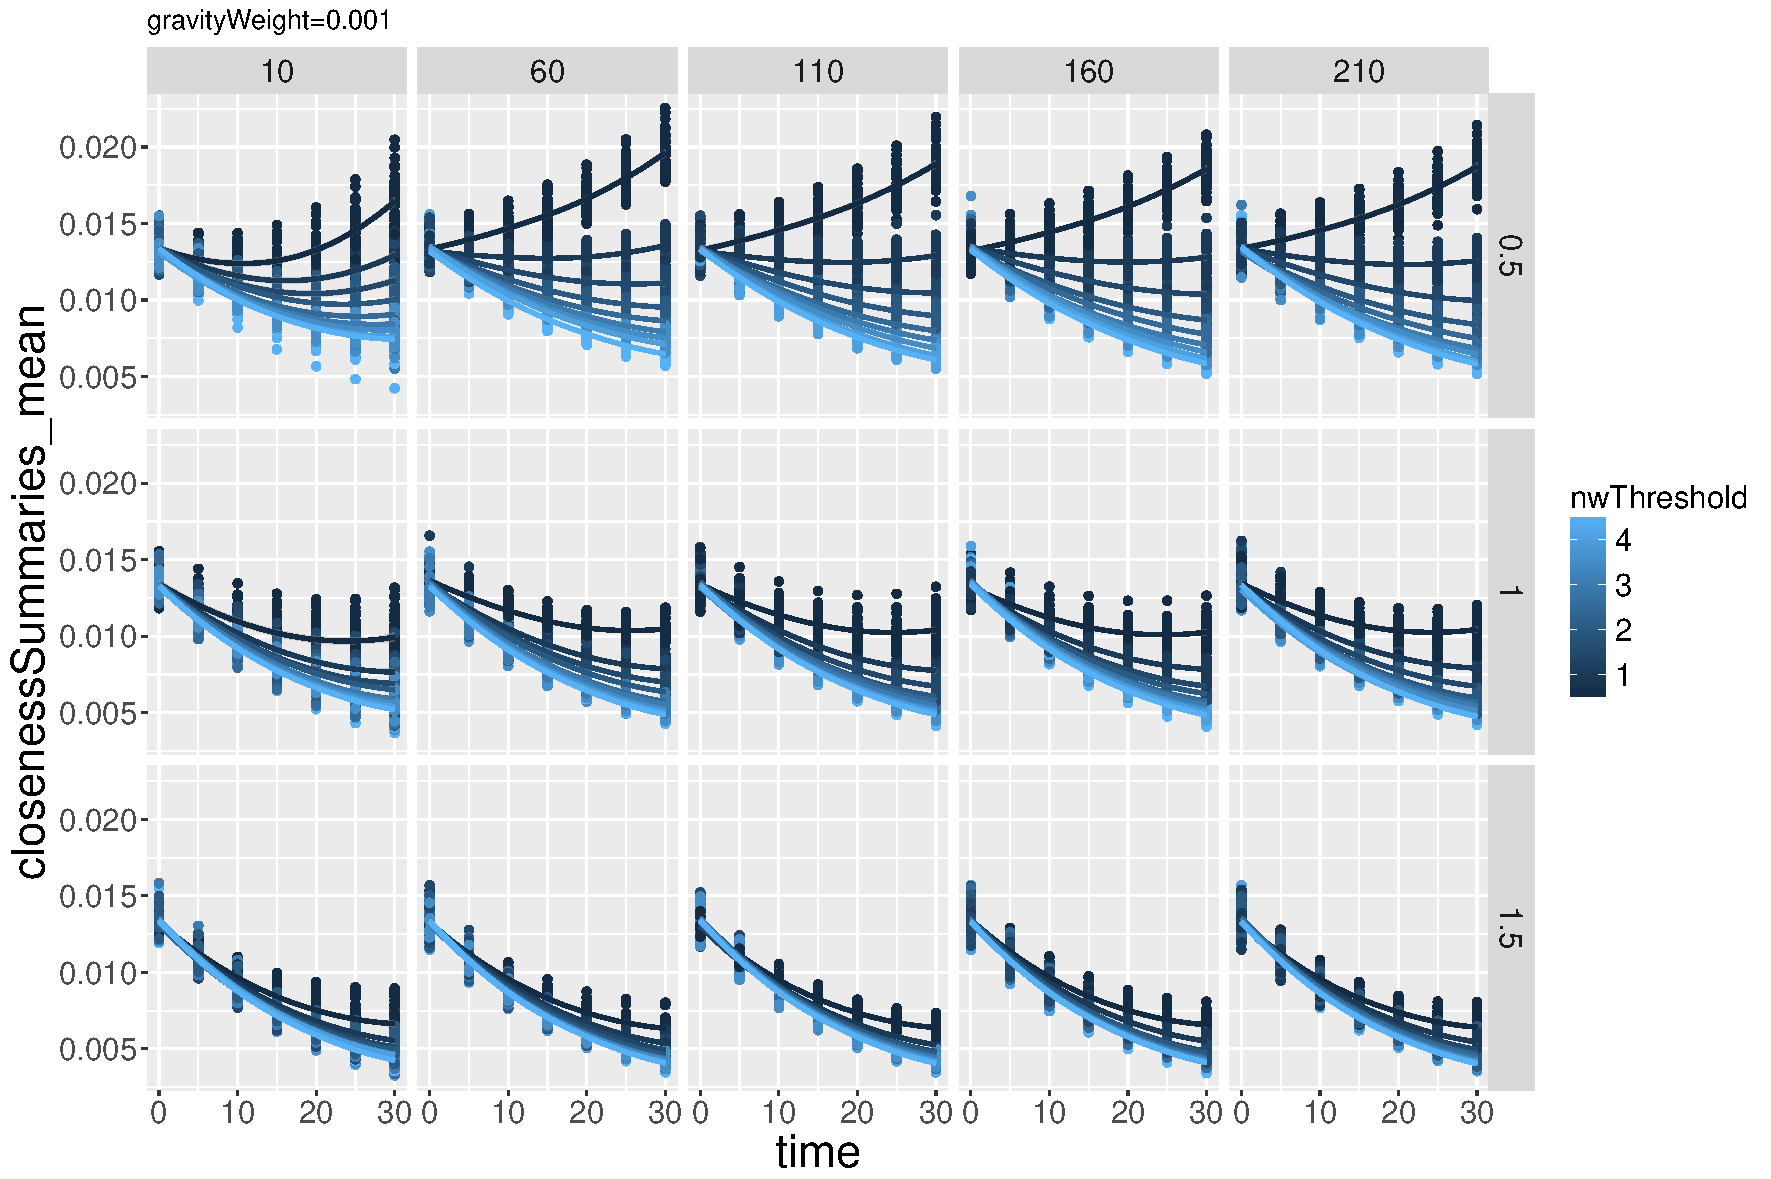
\includegraphics[width=0.48\linewidth]{Figures/MacroCoEvol/closenessSummaries_mean_gravityWeight0_001}
%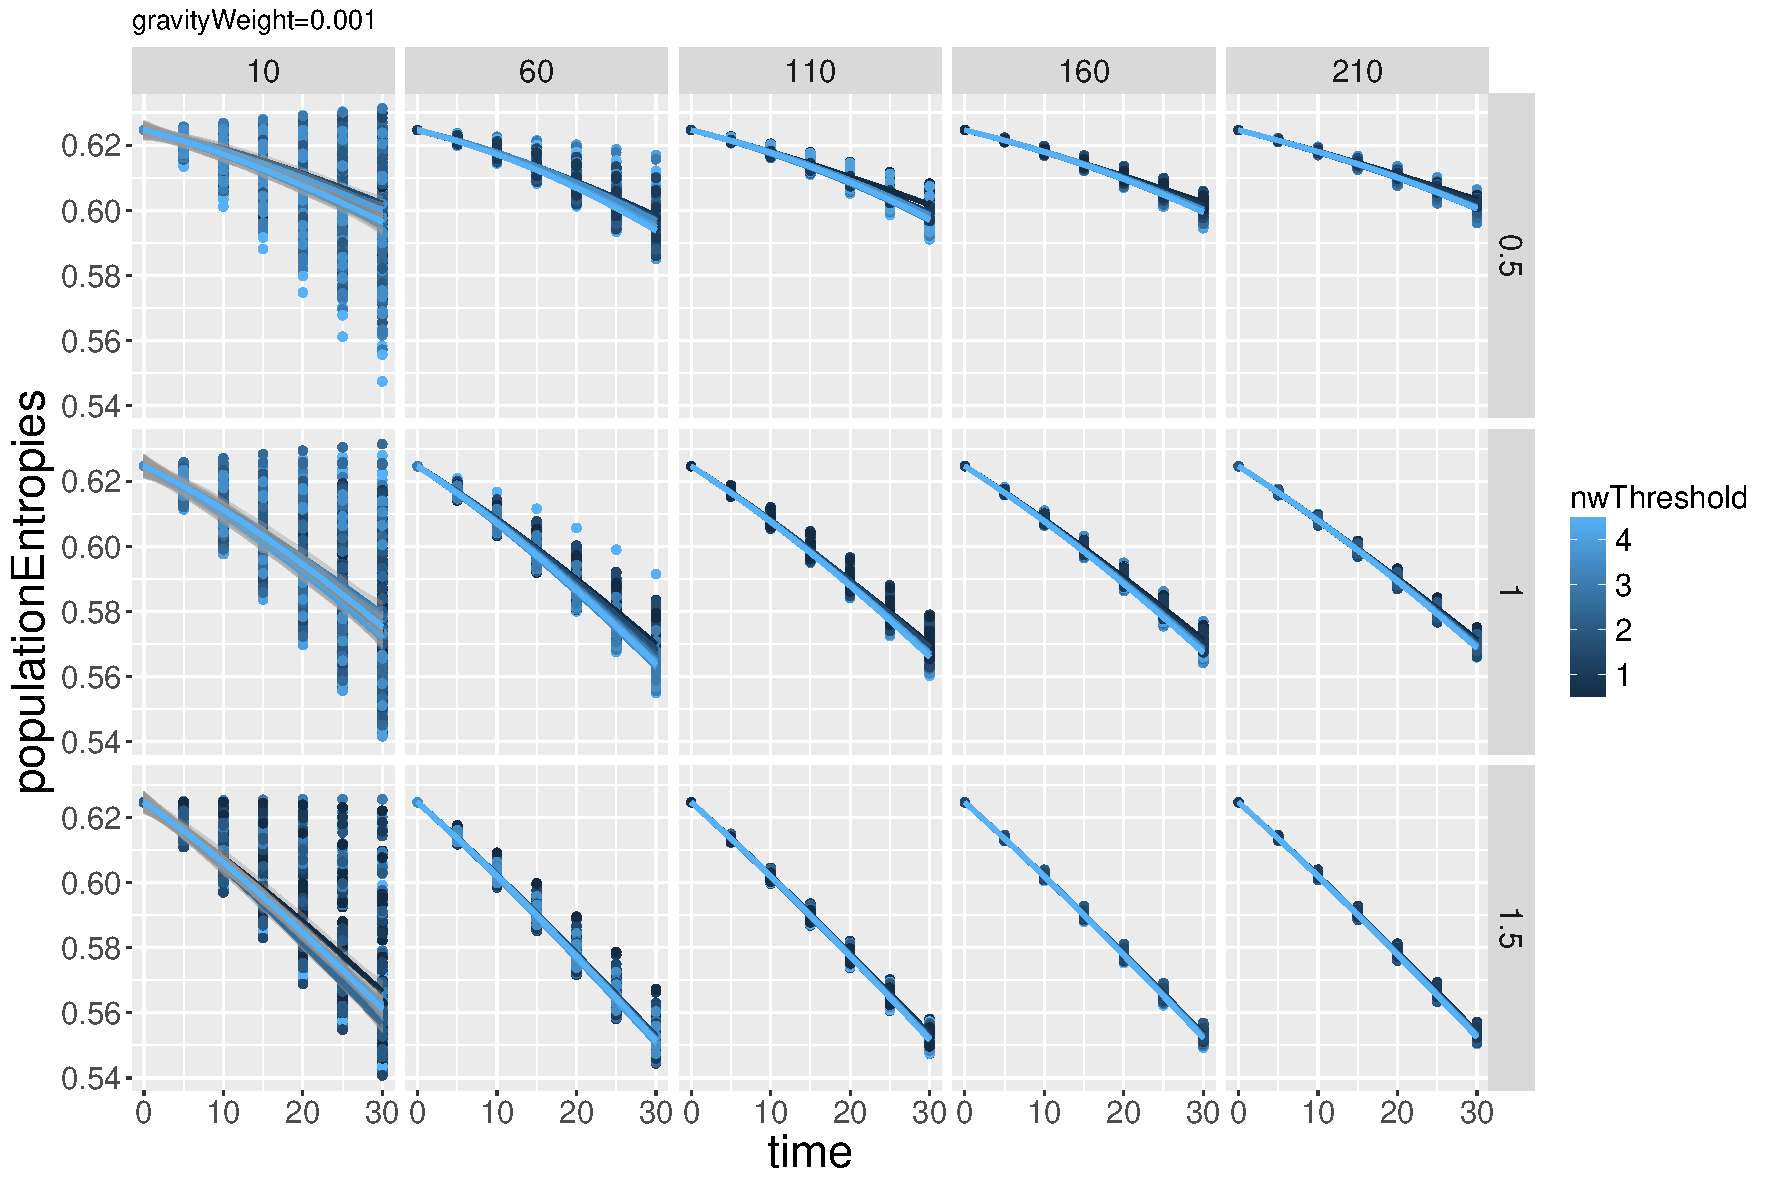
\includegraphics[width=0.48\linewidth]{Figures/MacroCoEvol/populationEntropies_gravityWeight0_001}\\
%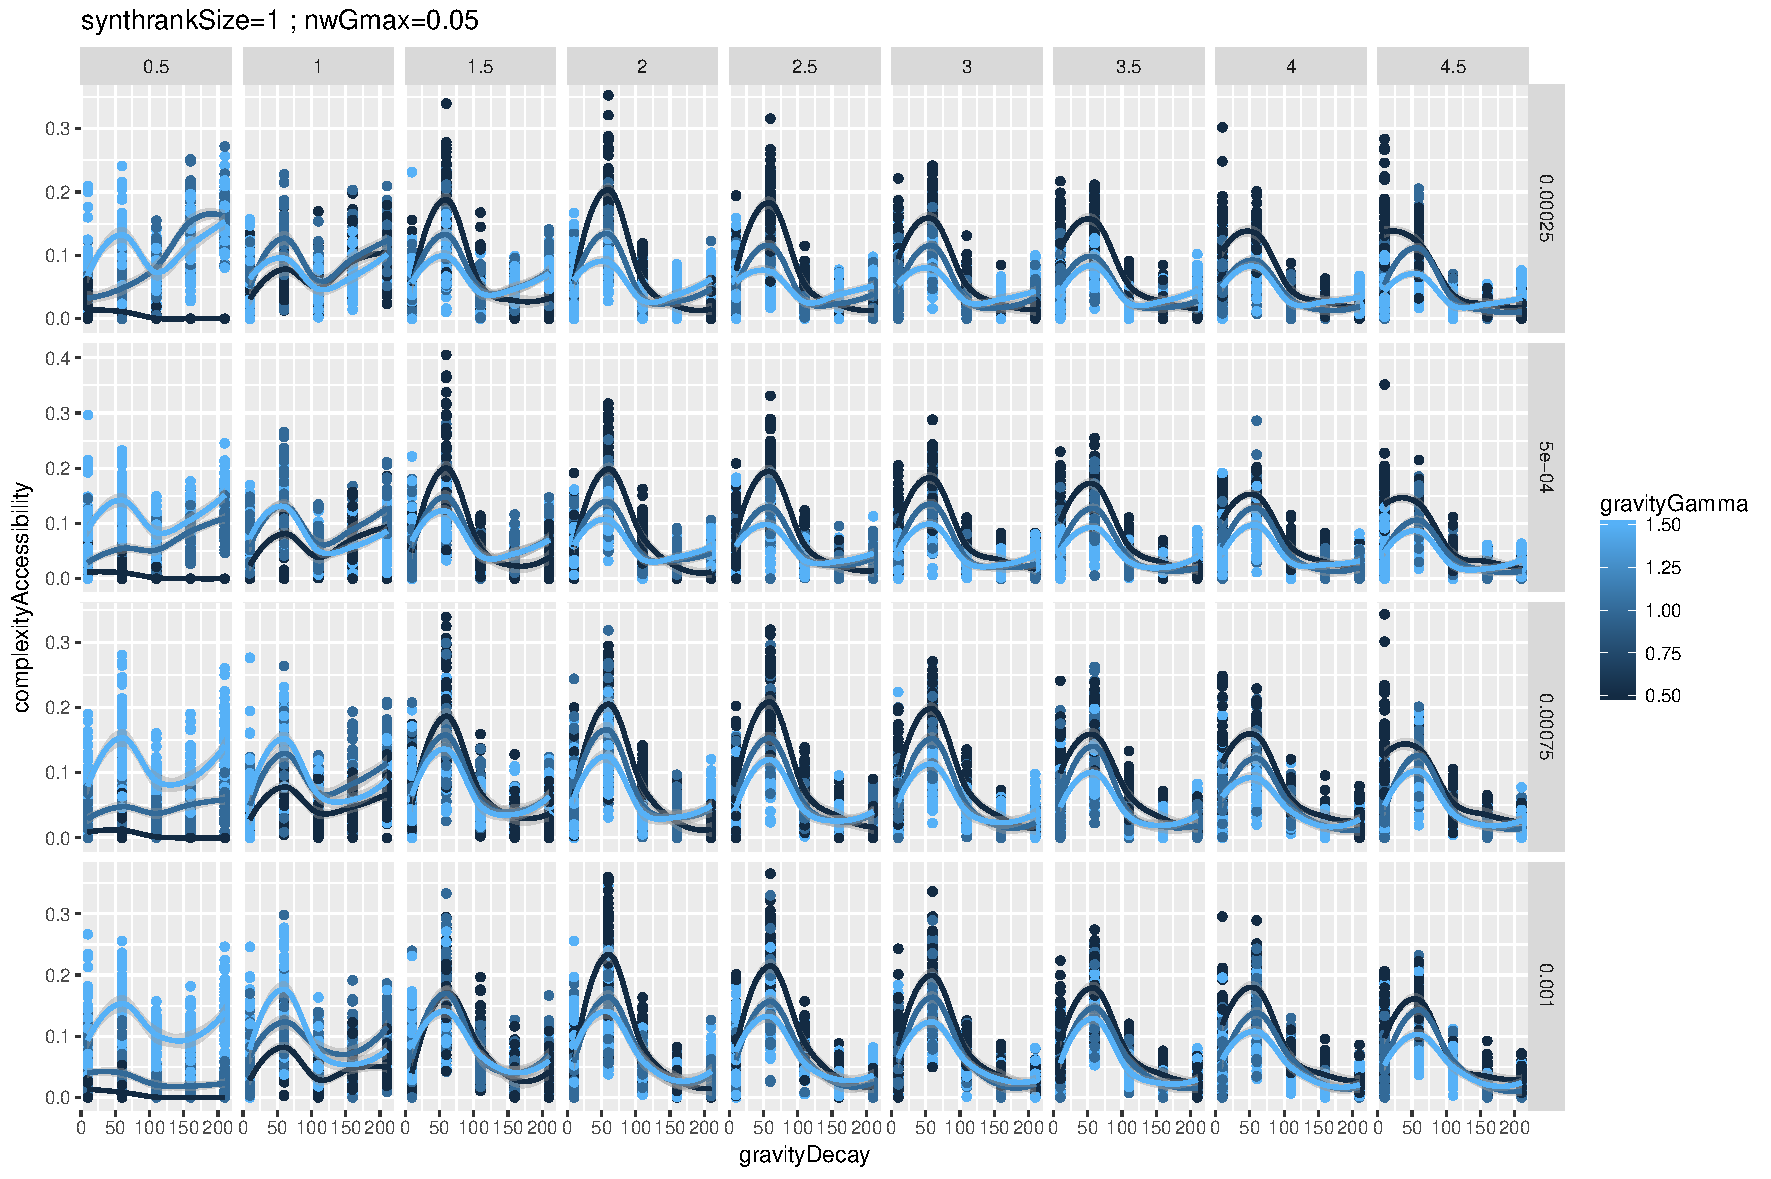
\includegraphics[width=0.48\linewidth]{Figures/MacroCoEvol/complexityAccessibility_synthrankSize1_nwGmax0_05}
%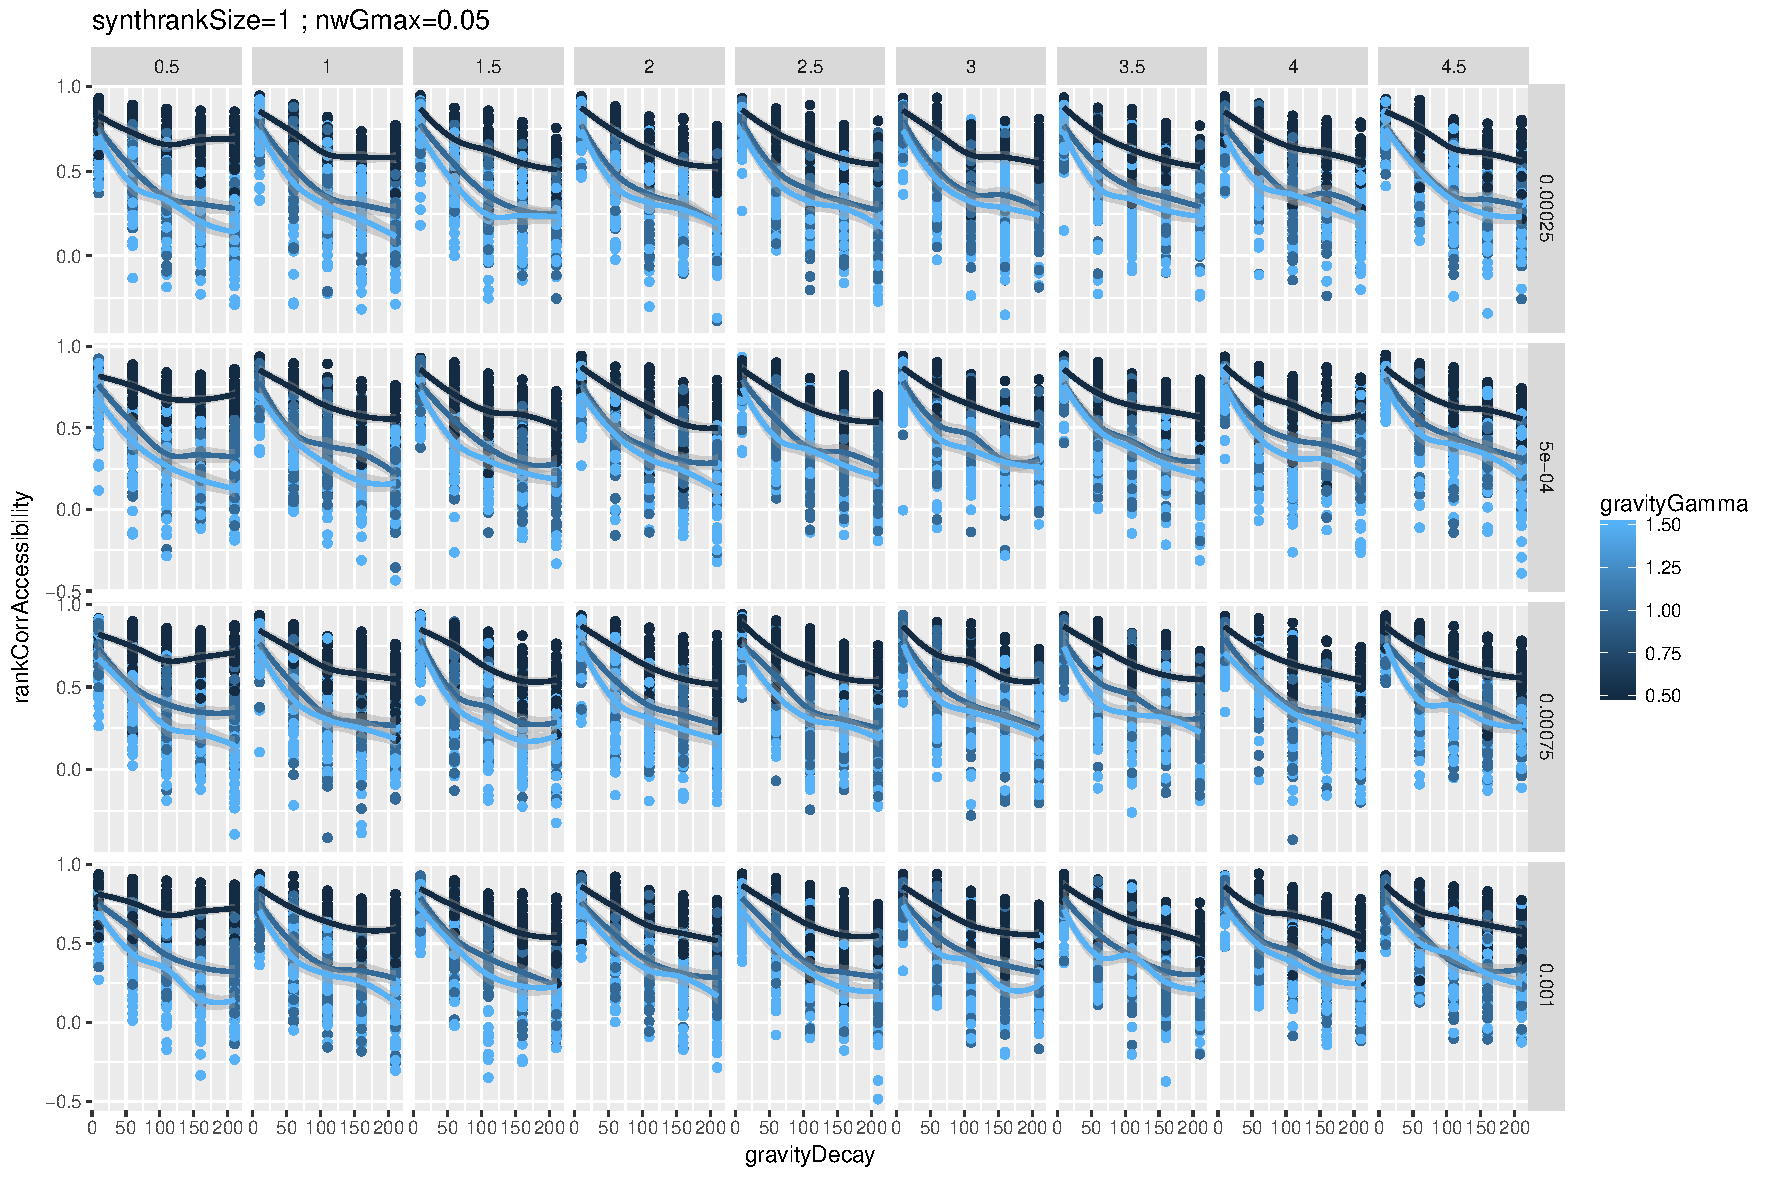
\includegraphics[width=0.48\linewidth]{Figures/MacroCoEvol/rankCorrAccessibility_synthrankSize1_nwGmax0_05}
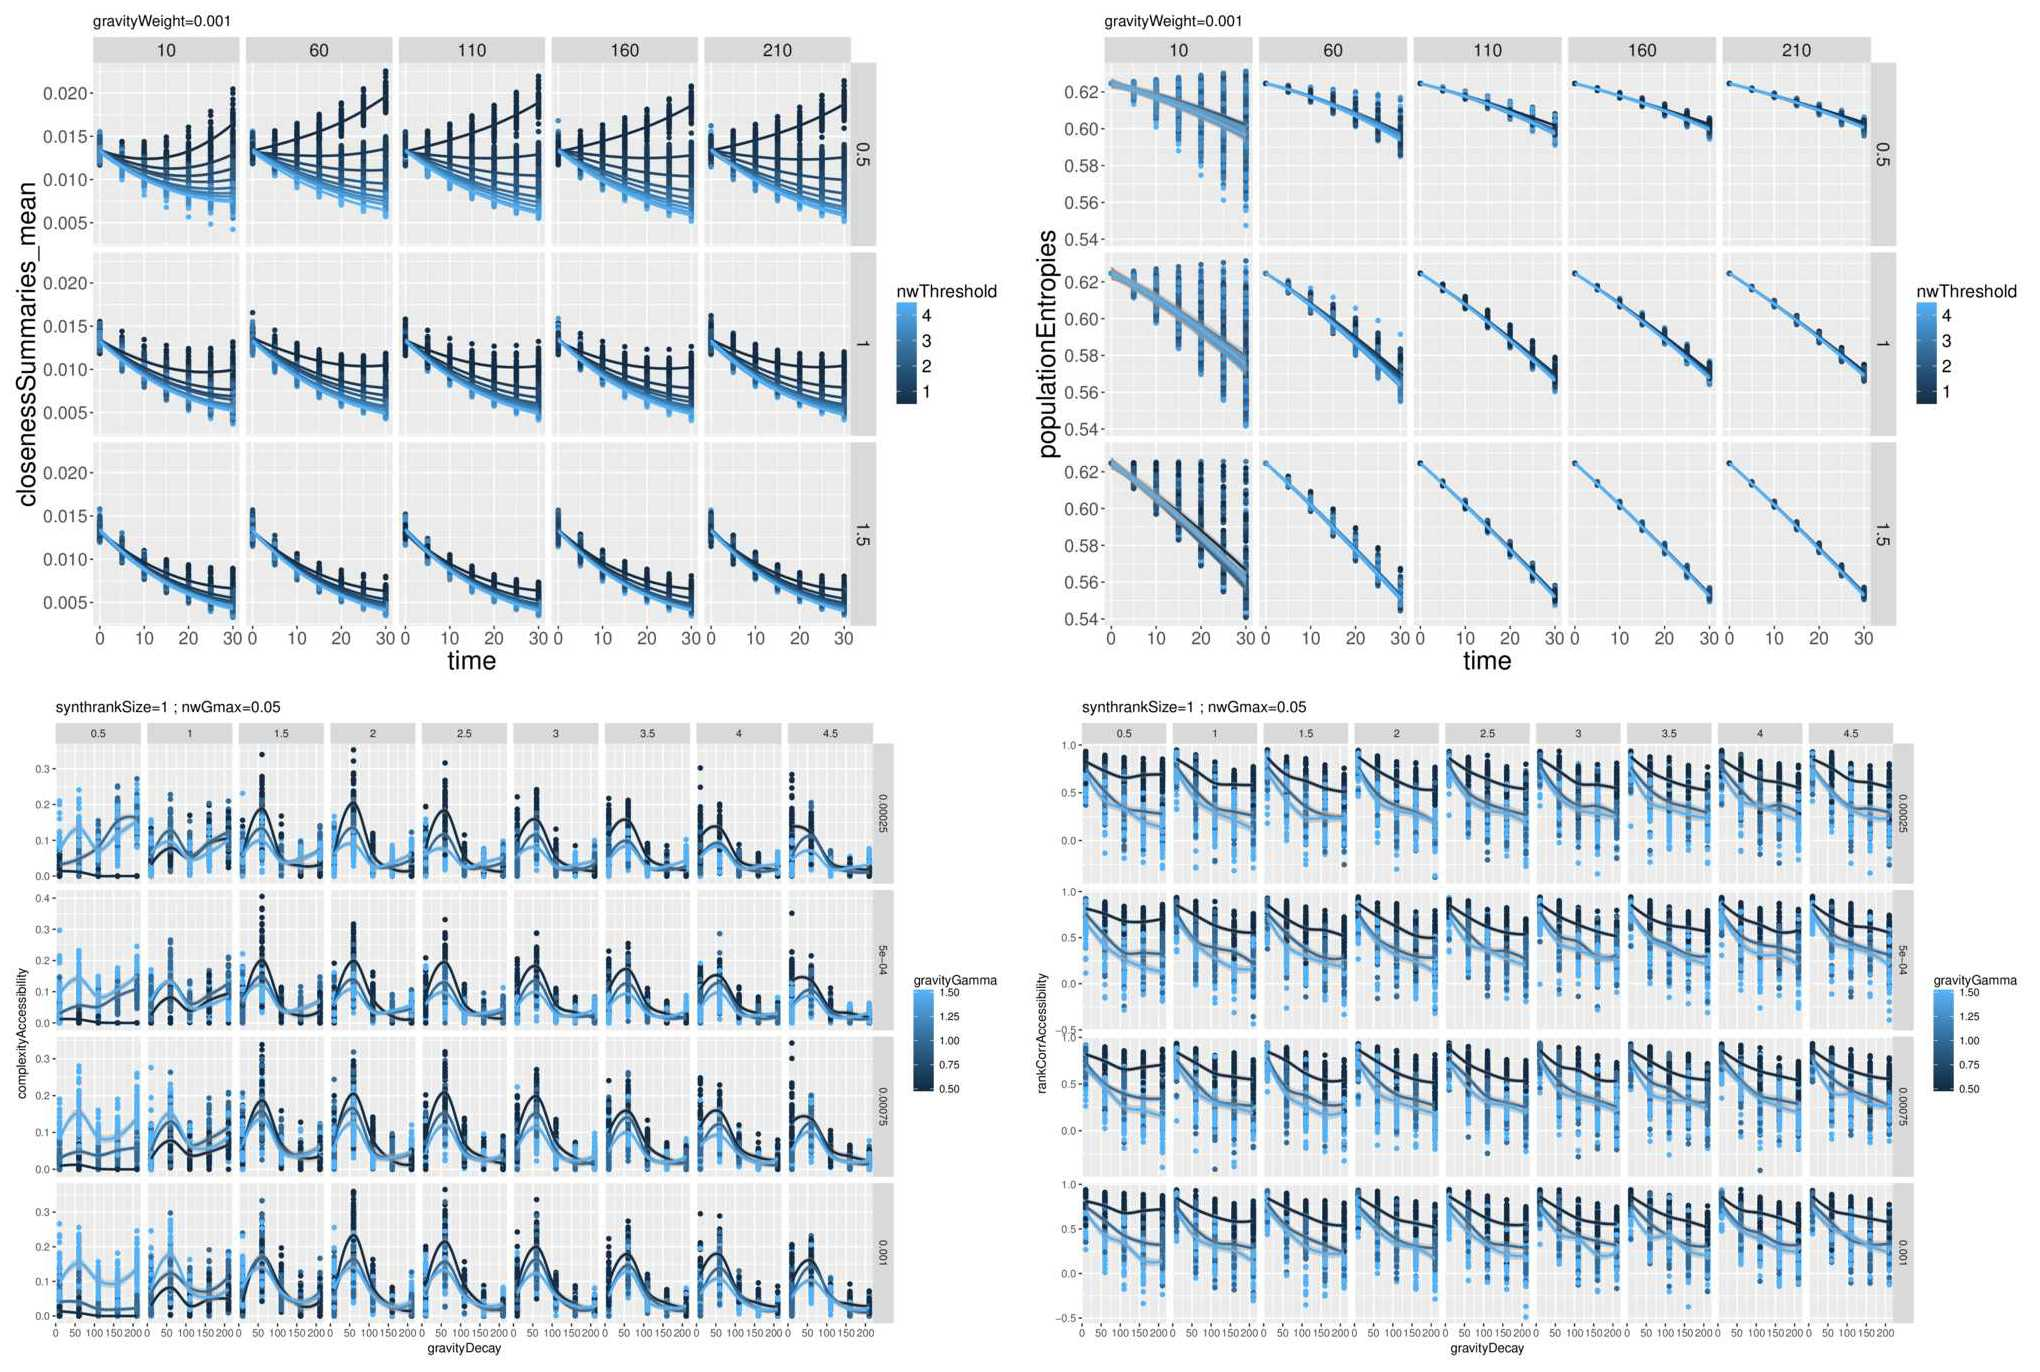
\includegraphics[width=\linewidth]{Figures/Final/6-2-2-fig-macrocoevol-behavior.jpg}
\caption[Behavior of the co-evolution model][Comportement du modèle de co-evolution]{\textbf{Behavior of the co-evolution model.}\label{fig:macrocoevol:behavior}}{\textbf{Comportement du modèle de co-evolution avec réseau abstrait sur un système de villes synthétique, pour $\alpha_S = 1$.} \textit{(Haut Gauche)} Moyenne des centralités de proximité, en fonction du temps, pour $d_G$ (colonnes), $\gamma_G$ (lignes) et $\phi_0$(couleur) variables, à $w_G = 0.001$ fixé ; \textit{(Haut Droite)} Entropie de populations, en fonction du temps, pour $d_G$ (colonnes), $\gamma_G$ (lignes) et $\phi_0$(couleur) variables, à $w_G = 0.001$ fixé ; \textit{(Bas Gauche)} Complexité des accessibilités, en fonction de $d_G$, pour $\phi_0$ (colonnes), $w_G$ (lignes) et $\gamma_G$ (couleur) variables ; \textit{(Bas Droite)} Corrélations de rang des accessibilités, pour les mêmes paramètres. Se référer au texte pour l'interprétation.\comment[AB]{illisible}\comment[FL]{()}\label{fig:macrocoevol:behavior}}
\end{figure}
%%%%%%%%%%%%%




%%%%%%%%%%%%%
\begin{figure}
	%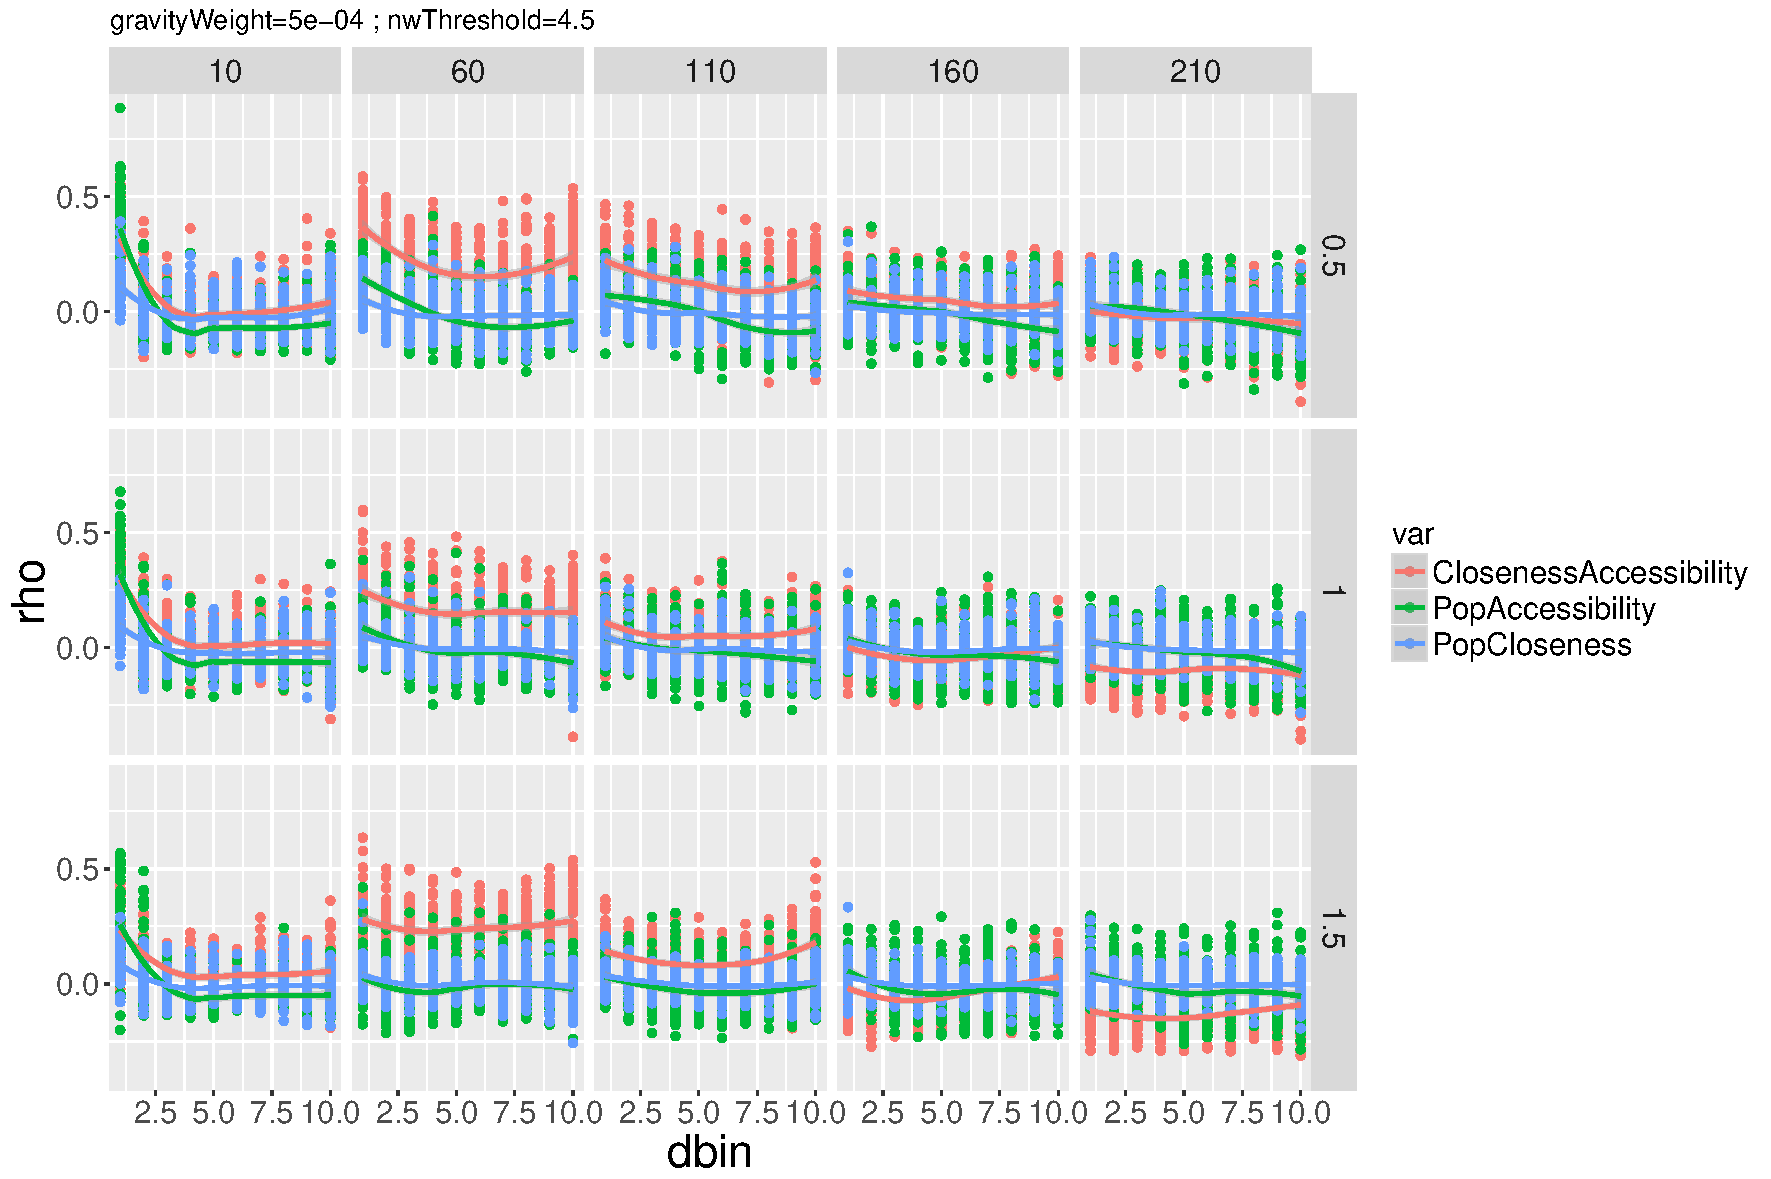
\includegraphics[width=0.9\linewidth]{Figures/MacroCoEvol/distcorrs_gravityWeight5e-04_nwThreshold4_5}\\
	%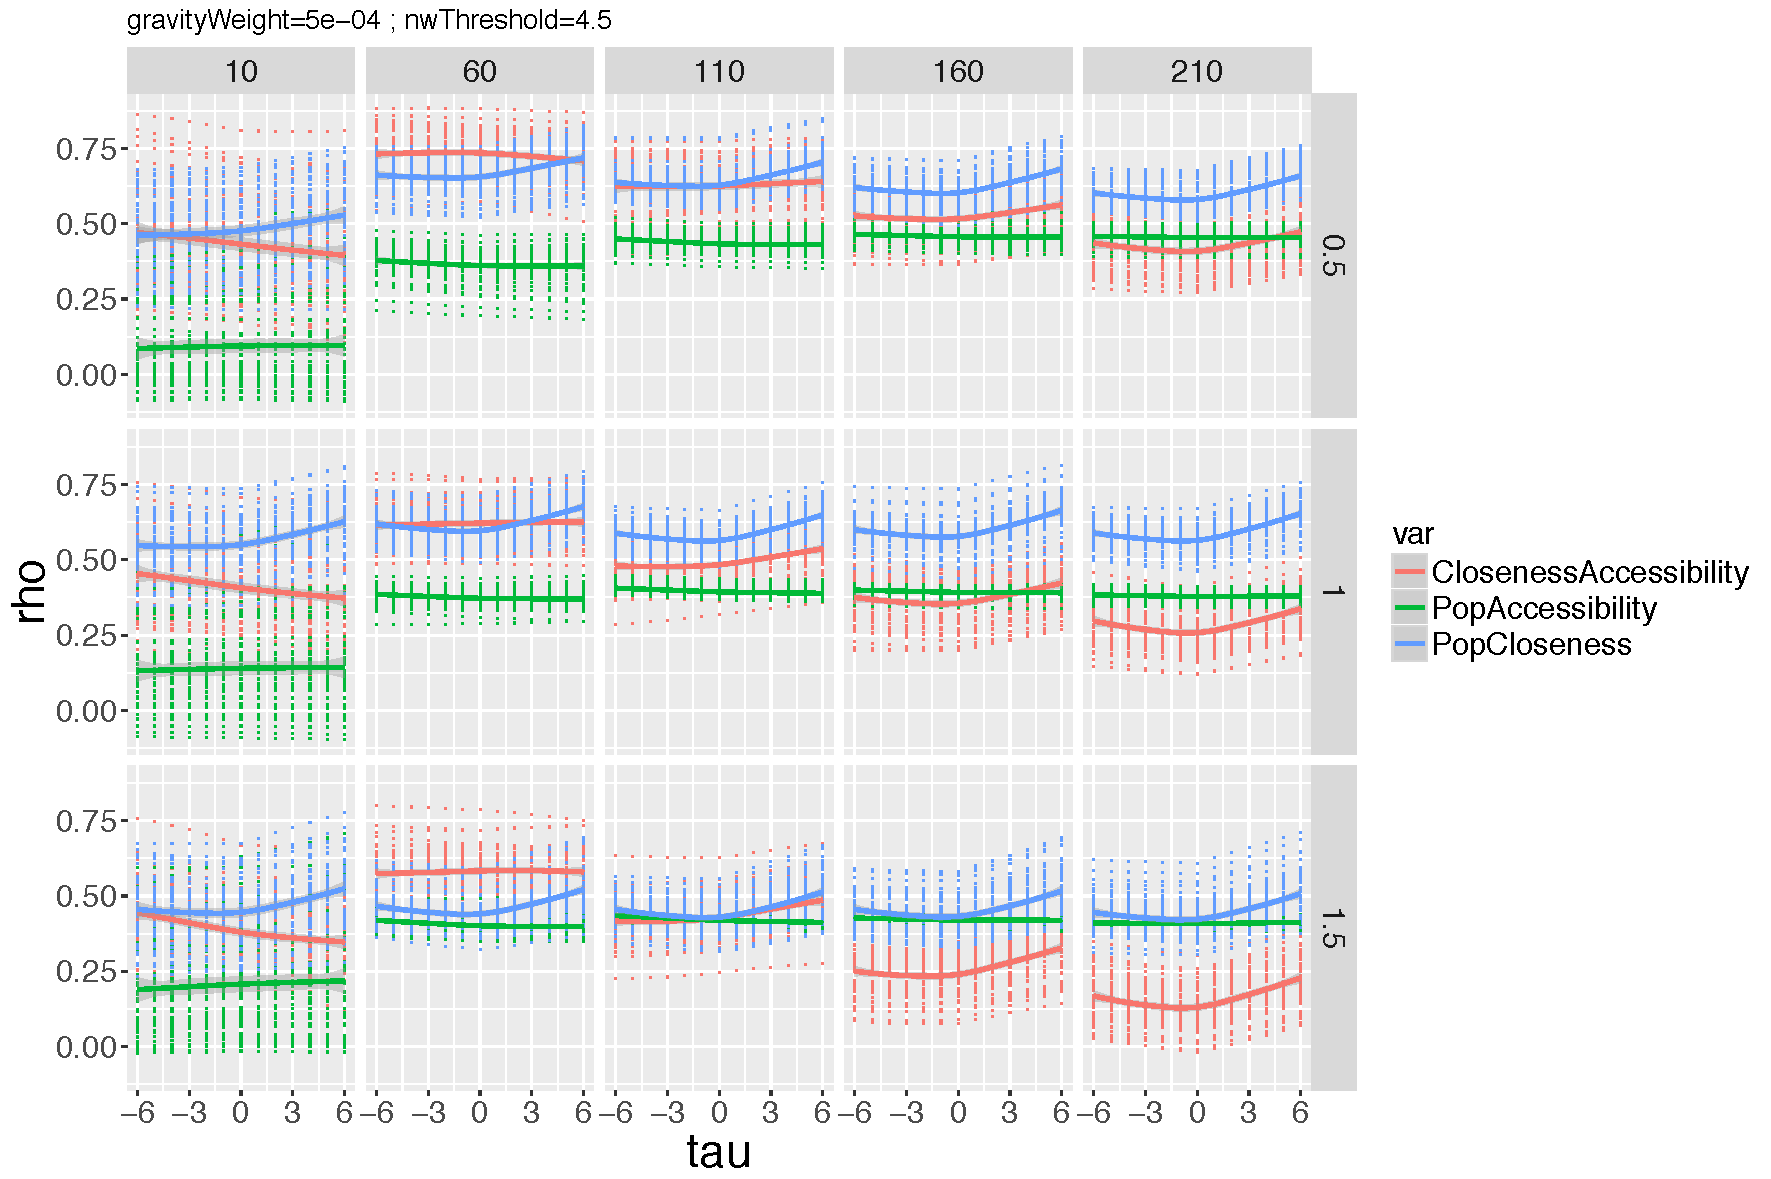
\includegraphics[width=0.9\linewidth]{Figures/MacroCoEvol/laggedcorrs_gravityWeight5e-04_nwThreshold4_5}
	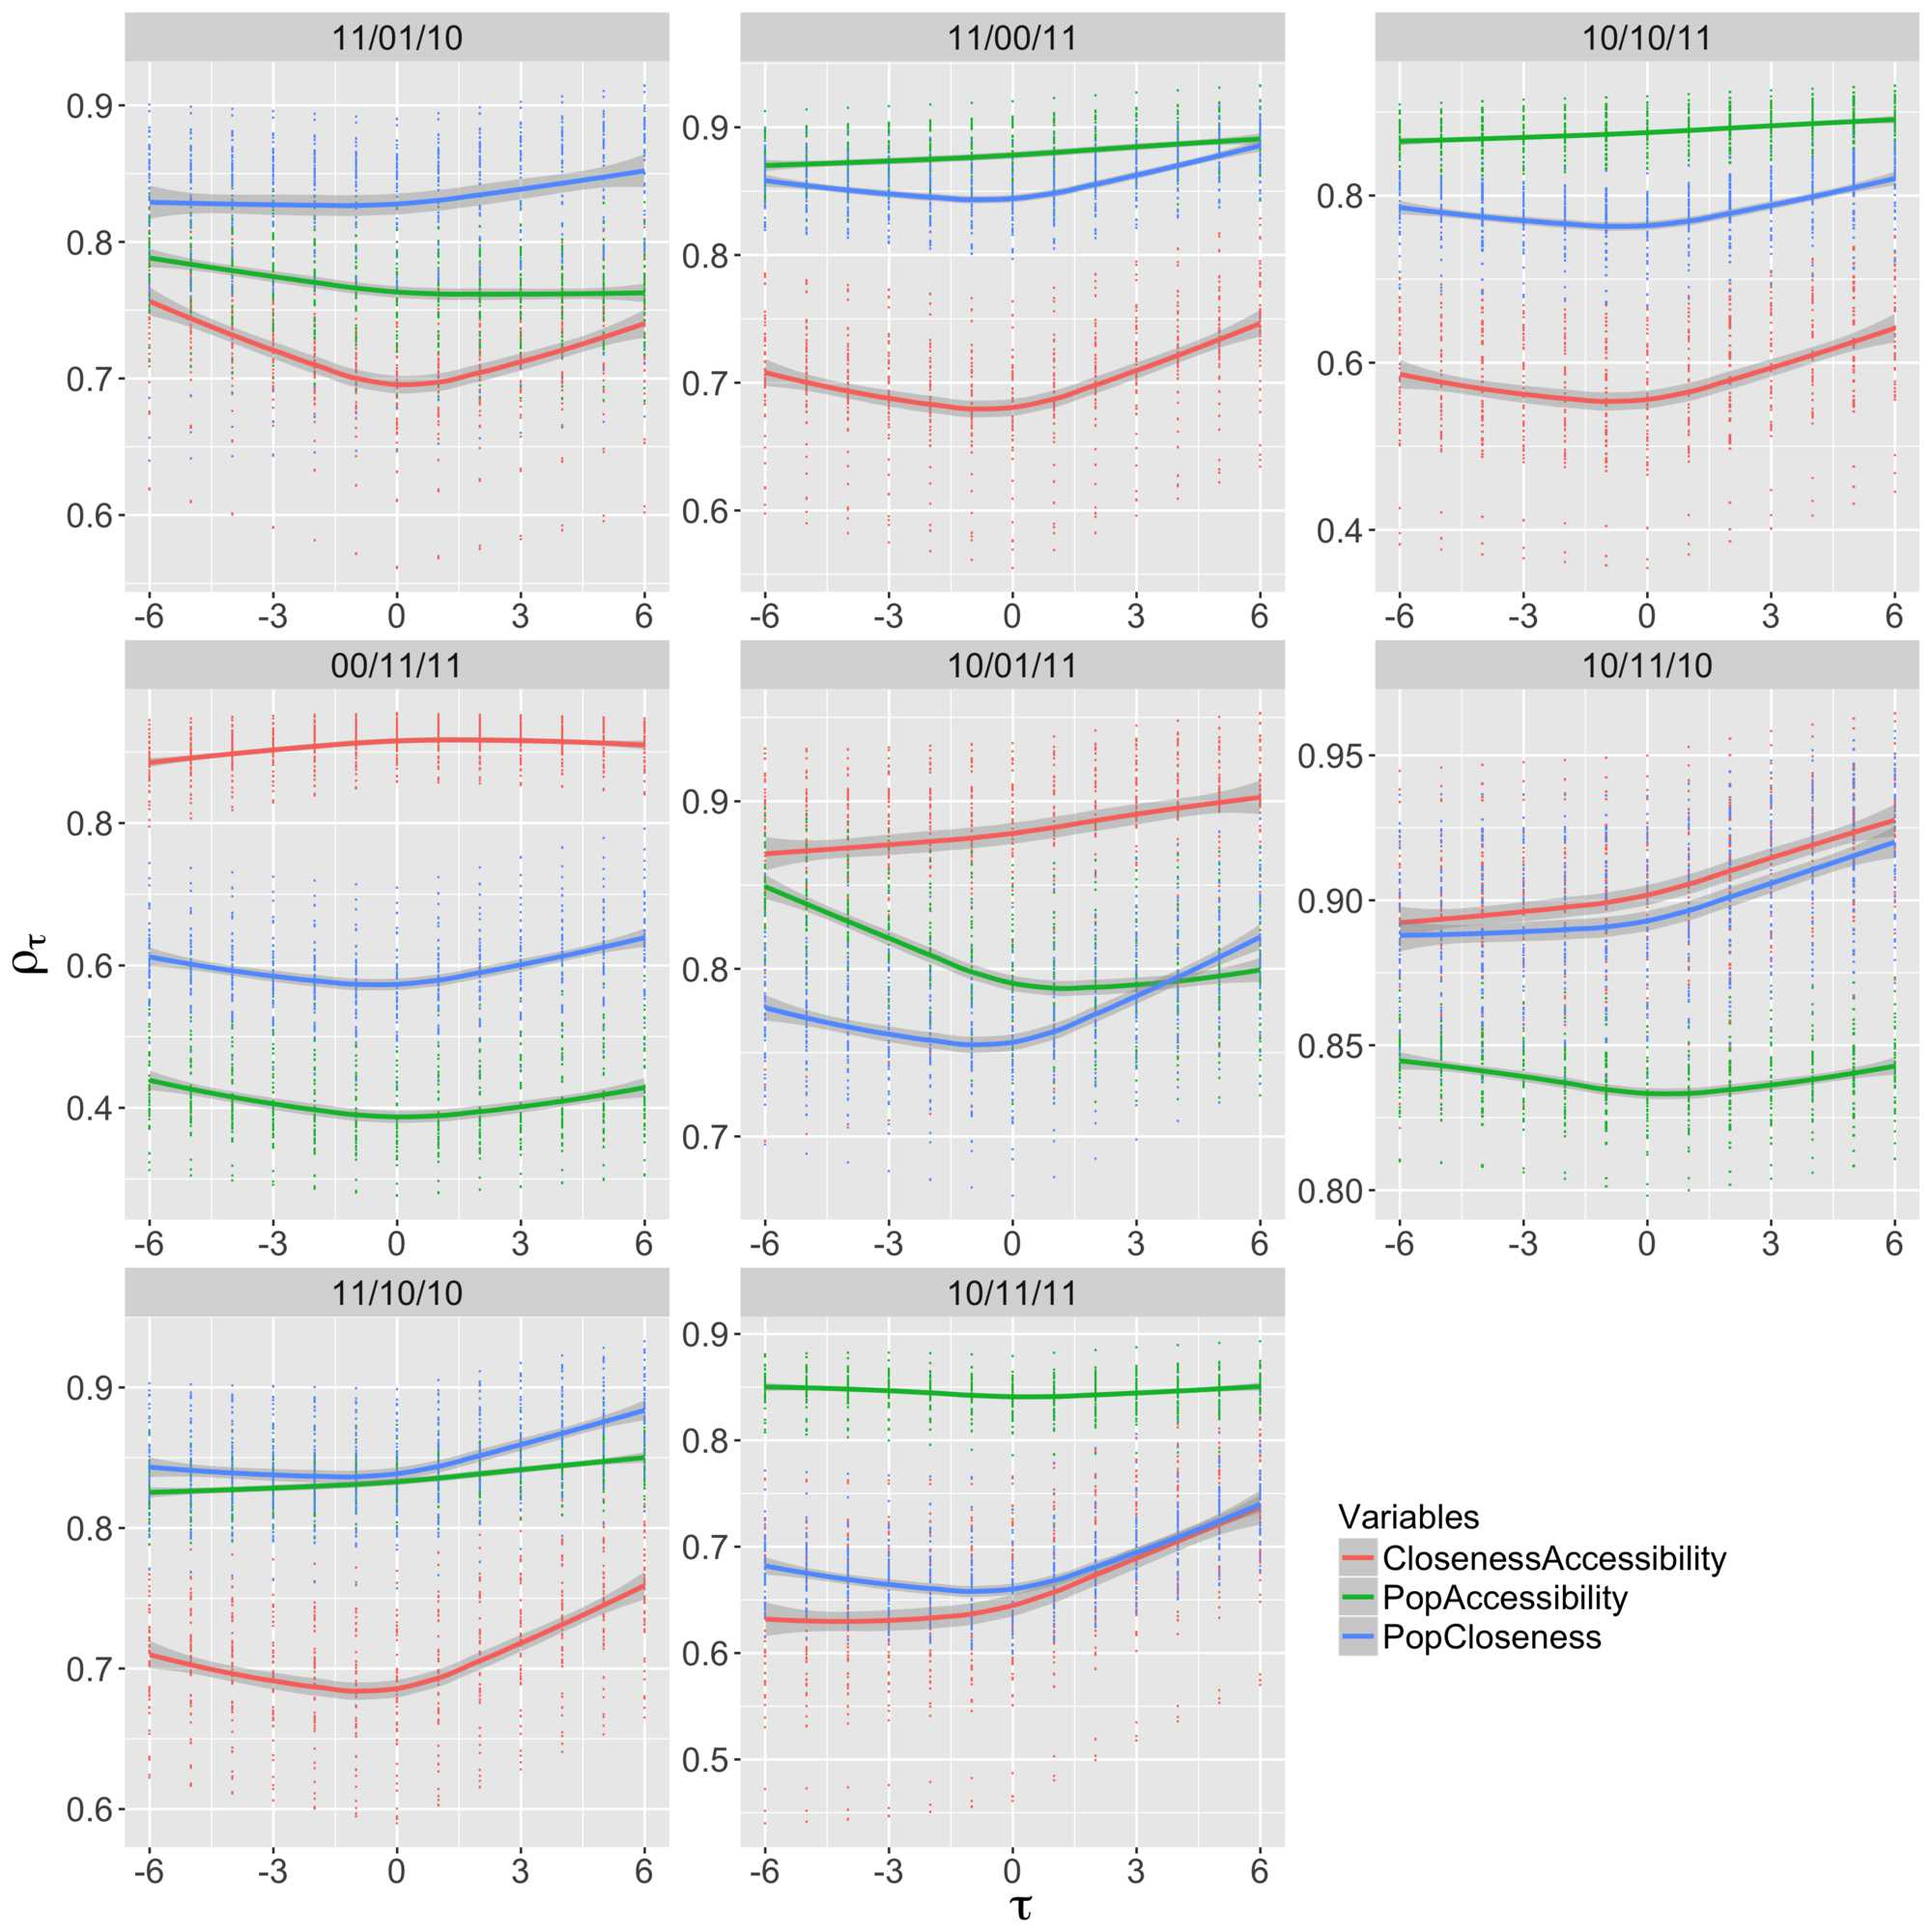
\includegraphics[width=\linewidth,height=0.8\textheight]{Figures/Final/6-2-2-fig-macrocoevol-correlations.jpg}
\caption[Correlations in the abstract model][Correlations dans le modèle abstrait]{}{\textbf{Motifs de correlation dans le modèle abstrait.} \textit{(Haut)} Correlation $\rho_d$ entre couples de variables (donné par la couleur), en fonction de la distance $d$ (discrétisée en déciles), pour $d_G$ variable (colonnes) et $\gamma_G$ variable (lignes), à $w_G = 5e-4$ et $\phi_0 = 4.5$ ; \textit{(Bas)} Correlations retardées $\rho_{\tau}$ en fonction du retard $\tau$, de manière similaire pour $d_G$ variable (colonnes) et $\gamma_G$ variable (lignes), à $w_G = 5e-4$ et $\phi_0 = 4.5$.\comment[AB]{Test Stat ; Idem} \label{fig:macrocoevol:correlations}}
\end{figure}
%%%%%%%%%%%%%


Tournons nous à present vers les motifs de corrélation produits par le modèle, illustrés en Fig.~\ref{fig:macrocoevol:correlations}. En fonction de la distance, les profils de $\rho_d$ pour les trois couples de variables montrent que des valeurs moyennes et grandes de la distance d'interaction ($d_G > 50$) décorrèlent\comment[FL]{md} totalement population avec centralité et accessibilité. Pour des petits $d_G$, un profil décroissant puis nul confirme l'existence d'effets locaux forts, où des villes très proches s'influenceront fortement. Le comportement de la correlation entre accessibilité et centralité est plus difficile à interpréter, et peut être dû aux phénomènes d'auto-correlation\footnote{qui ne sont pas calculables, car il s'agirait de décomposer $\rho\left[\sum_{i\neq j} \frac{1}{d_{ij}}; \sum_{i\neq j} P_j \exp{\left(-d_{ij}/d_G\right)}\right]$. Il est possible par exemple d'approximer $\rho\left[X+Y;Z\right]$ sous la condition que $\varepsilon = \sigma_Y / \sigma_X \ll 1$ au premier ordre par $\rho\left[ X+Y;Z \right] \simeq \rho\left[ X;Z \right]\left(1+\frac{1}{2}\rho\left[X;Y\right]\varepsilon - \frac{\varepsilon^2}{2})\right) + \varepsilon \rho\left[Y;Z\right]$, mais cette hypothèse est trop restrictive pour être valable sur l'ensemble de la somme.}. Son niveau ne dépend pas de la distance mais de $d_G$, et est décroissant pour finir à une corrélation négative. Enfin, concernant les corrélations retardées, on observe systématiquement une déviation positive de la corrélation entre population et accessibilité pour les retards positifs, en croissance jusqu'au retard maximal, ce qui pourrait être un marqueur du renforcement des dynamiques de population par la centralité, fait stylisé exhibé pour le système de ville Français par~\cite{bretagnolle:tel-00459720}. La correlation entre population et accessibilité est constante, probablement par l'auto-corrélation, et n'entre pas en jeu dans la définition des régimes. Pour des valeurs intermédiaires de $d_G$ et les fortes valeurs de $\gamma_G$, on observe également une très légère déviation pour les retards négatifs : pour ces régimes, on a causalité circulaire et le modèle capture une co-évolution dans ce sens. L'accessibilité quant à elle cause fortement la centralité pour $d_G = 10$, puis la tendance s'inverse pour les grands $d_G$. Pour $d_G = 10$, cela va dans le sens du lien entre population et centralité, et il n'y a dans ce cas pas co-évolution mais adaptation des populations au réseau.\comment[FL]{il faut harmoniser les termes ici : relation univoque est plus generique ?} Pour les régimes intermédiaire, on a circularité directement entre population et centralité, tandis que pour $d_G > 110$ il y a ``circularité indirecte'', puisque accessibilité cause centralité qui cause population (qui entre en jeu dans la centralité). Ainsi, le modèle capture au moins trois régimes de co-évolution distincts, en fonction de la distance d'interaction et du niveau de hiérarchie\footnote{Une analyse plus systématique par apprentissage non-supervisé comme en~\ref{sec:causalityregimes} et en~\ref{sec:mesocoevolmodel} est laissée pour de futures développements.}.


\comment[AB]{trop abstrait}



\paragraph{Synthesis}{Synthèse}

Les faits stylisés marquants qui ressortent de l'exploration du modèle synthétique sont les suivants :

\begin{enumerate}
	\item On révèle l'existence d'une échelle spatiale intermédiaire permettant l'évolution de niches\comment[AB]{definir} relativement indépendantes, correspondant à un niveau de complexité des trajectoires maximal.
	\item Les corrélations retardées mettent en évidence au moins trois régimes différents d'interaction, que l'on interprète comme un régime d'adaptation, un régime de co-évolution direct et un régime de co-évolution indirecte.\comment[FL]{c'est crucial, peut etre plutot dans une partie theorique "a quoi peut-on s'attendre" ?}
\end{enumerate}

reproduction du first mover advantage ? \cite{levinson2011does}



%%%%%%%%%%%%%%%%%
%\subsection[Application][Application]{Applications to Case Studies}{Applications au Système de Villes Français}
\subsection{Applications to French City System}{Applications au Système de Villes Français}



\bpar{
The model is applied to the French Urban System on long time dynamical data : Pumain-INED database for populations spanning between 1831 and 1999, with the evolving railway network from 1840 to 2000.
}{
Le modèle est ensuite appliqué au système de villes français sur des données dynamiques sur le temps long : la base Pumain-INED pour les populations, couvrant de 1831 à 1999, avec le réseau ferré dynamique de 1840 à 2000.\comment[AB]{sources} Cette application vise d'une part à tester la capacité du modèle à reproduire une dynamique de co-évolution réelle, et d'autre part à extraire une information thématique sur les processus via les valeurs calibrées des paramètres.\comment[FL]{pourquoi est-il pertinent / necessaire de travailler avec ce recul temporel ?}
}



\subsubsection{Network Data}{Données de Réseau}

Nous travaillons sur les données de réseau ferré construites par~\cite{thevenin2013mapping}. Le réseau ferré français est particulièrement intéressant en conjonction avec les données de population déjà présentées, puisque la période couverte est relativement similaire, et que ce moyen de transport a à toute période concrétisé l'implication d'acteurs publiques et privés importants, tout en exhibant\comment[AB]{qu'appelles tu exhiber ici ? patterns ? processus ?} différents régimes selon les époques, d'une gestion plutôt décentralisée à une centralisation très forte plus récemment, et différentes concrétisations technologiques avec par exemple l'émergence récente de la grande vitesse.\comment[AB]{references} Pour chaque date de la base de donnée de population, nous extrayons le graphe abstrait simplifié où toutes les gares et intersections de degré supérieur à deux sont reliés par les liens abstrait avec attributs de vitesse et distance traduisant la valeur réelle, à une granularité de 1km. Cela permet également de construire les matrice de distance-temps entre les villes considérées dans le modèle.\comment[AB]{mieux mettre en valeur}

\comment[FL]{developpe cette partie pour mieux la mettre en valeur}




\subsubsection{Stylized facts}{Faits stylisés}


Avant de calibrer le modèle, observons les motifs de corrélation présents dans les données, en appliquant la méthode des corrélations retardées. Cette étude empirique devrait permettre d'une part de vérifier des faits stylisés connus, d'autre part d'établir une connaissance préliminaire du comportement empirique du système. Nous calculons comme précisé ci-dessus la centralité de proximité via le réseau, donnée par $T_i = \sum_j \exp{-d_{ij}/d_0}$, et étudions la corrélation retardée entre sa dérivée $\Delta T_i$ et celle de la population $\Delta P_i$, donnée par $\hat{\rho}_{\tau} = \hat{\rho}\left[\Delta P_i(t),\Delta T_i(t-\tau)\right]$ estimée sur une fenêtre glissante comprenant $T_w$ dates successives. Nous montrons en Fig.~\ref{fig:macrocoevol:empirical} les résultats obtenus. Ceux-ci sont conséquents\comment[AB]{:-)} pour au moins deux raisons. Dans un premier temps, le comportement du nombre de corrélations significatives en fonction de $T_w$ et de $d_0$ permet la recherche d'échelles de stationnarité dans le système. On observe d'une part une échelle spatiale spécifique donnant un maximum pour l'ensemble des fenêtres temporelles, à $d_0 = 100km$, ce qui suggère l'existence de sous-systèmes régionaux cohérents, dont l'existence est stable dans le temps\comment[FL]{rapide}. Celle-ci coincide remarquablement avec l'échelle intermédiaire isolée dans le modèle synthétique. D'autre part, les grandes portées spatiales induisent une échelle temporelle optimale, pour $T_w = 4$ ce qui correspond à une vingtaine d'année : nous l'identifions comme l'échelle de stationnarité temporelle du système dans son ensemble et étudions les corrélations retardées pour cette valeur. Dans un second temps, le comportement des corrélations retardées apporte une mauvaise nouvelle\comment[AB]{:-)} pour la littérature existante et pour les potentialités d'application de notre modèle.\comment[AB]{trop abstrait} A l'échelle spatiale intermédiaire, les valeurs de $\rho_+,\rho_-$ n'exhibent aucune régularité. Sur l'ensemble du système, on a jusqu'en 1946 quasiment aucun effet significatif, puis aucune causalité entre 1946 et 1975 (maximum à $\tau = 0$, minimum non significatif), puis un décalage de 5 an de l'accessibilité causant la population après 1968 (l'effet restant tout de même douteux). Nous ne reproduisons pas l'effet de corrélation entre centralité dans le réseau et place dans la hiérarchie urbaine défendu par~\cite{bretagnolle2003vitesse}\footnote{tout comme~\cite{lemoy2017scaling} n'arrivent pas à reproduire, pour les profils de densité en fonction de la distance au centre des métropoles européennes, la transition permettant à \cite{guerois2008built} de définir le péri-urbain. Ces travaux plus ou moins anciens ne sont pas reproductibles, ne fournissant ni code, ni données et ne donnant qu'une description très succincte des méthodes, et il est ainsi impossible de connaitre l'origine de la discrépance\comment[AB]{?} qualitative obtenue. Il devient urgent d'imposer la reproductibilité absolue comme critère \emph{sinequanone} de scientificité\comment[AB]{ca y'est tu reveles ton vrai visage :-)}, et de construire des comparaisons systématiques (\emph{bemchmarks}) de modèles, analyses empiriques, récentes mais aussi en validation d'études passées.}, ce qui amène à relativiser l'existence de la ``co-évolution structurelle'' sur le temps long décrite par \noun{Bretagnolle} dans~\cite{espacegeo2014effets}.\comment[AB]{expliciter systematiquement le lien} Nous rejoignons les résultats récents de~\cite{mimeur:hal-01616746} qui montrent le non-significativité statistique de la corrélation entre taux de croissance et évolution de la couverture du réseau ainsi que l'évolution de l'accessibilité, à délai nul. Nos résultats sont moins précis pour les classes de villes étudiées (ils différencient grandes villes et petites, et travaillent sur un panel plus grand), mais plus généraux car pour un délai et une portée de l'accessibilité variables, et donc complémentaires.



\comment[FL]{develpper et hierarchiser ce que tu retires, c'est clairement un endroit important de ta these : - se raccrocher aux hypotheses sur la coevolution a cette echelle ; se raccrocher aux hypotheses sur la facon de modeliser ce phenomene}


%%%%%%%%%%%%%
\begin{figure}
	%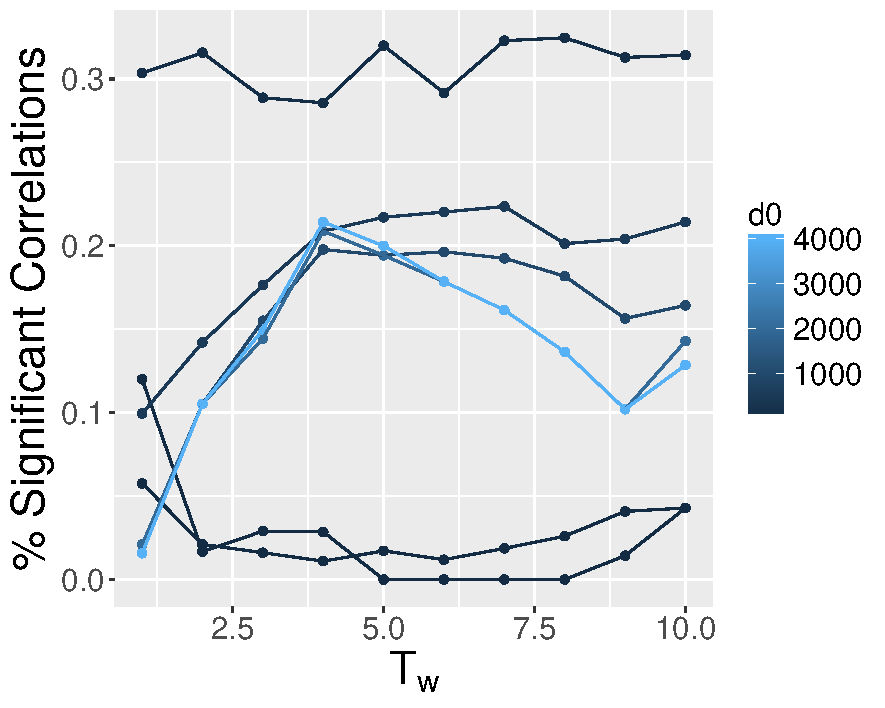
\includegraphics[width=0.48\linewidth]{Figures/MacroCoEvol/significantcorrs_Tw.pdf}
	%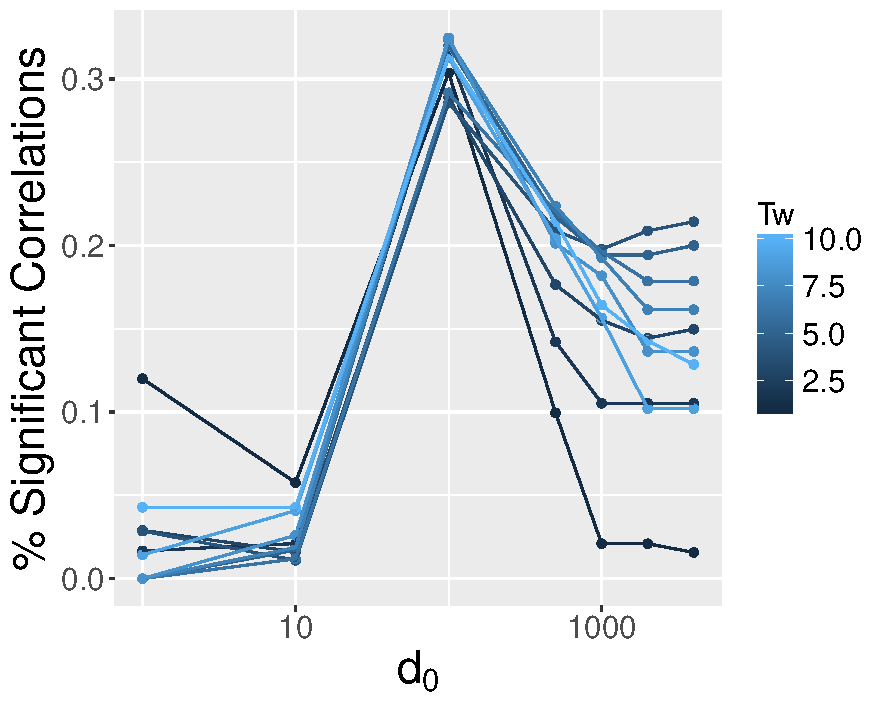
\includegraphics[width=0.48\linewidth]{Figures/MacroCoEvol/significantcorrs_d0.pdf}\\
	%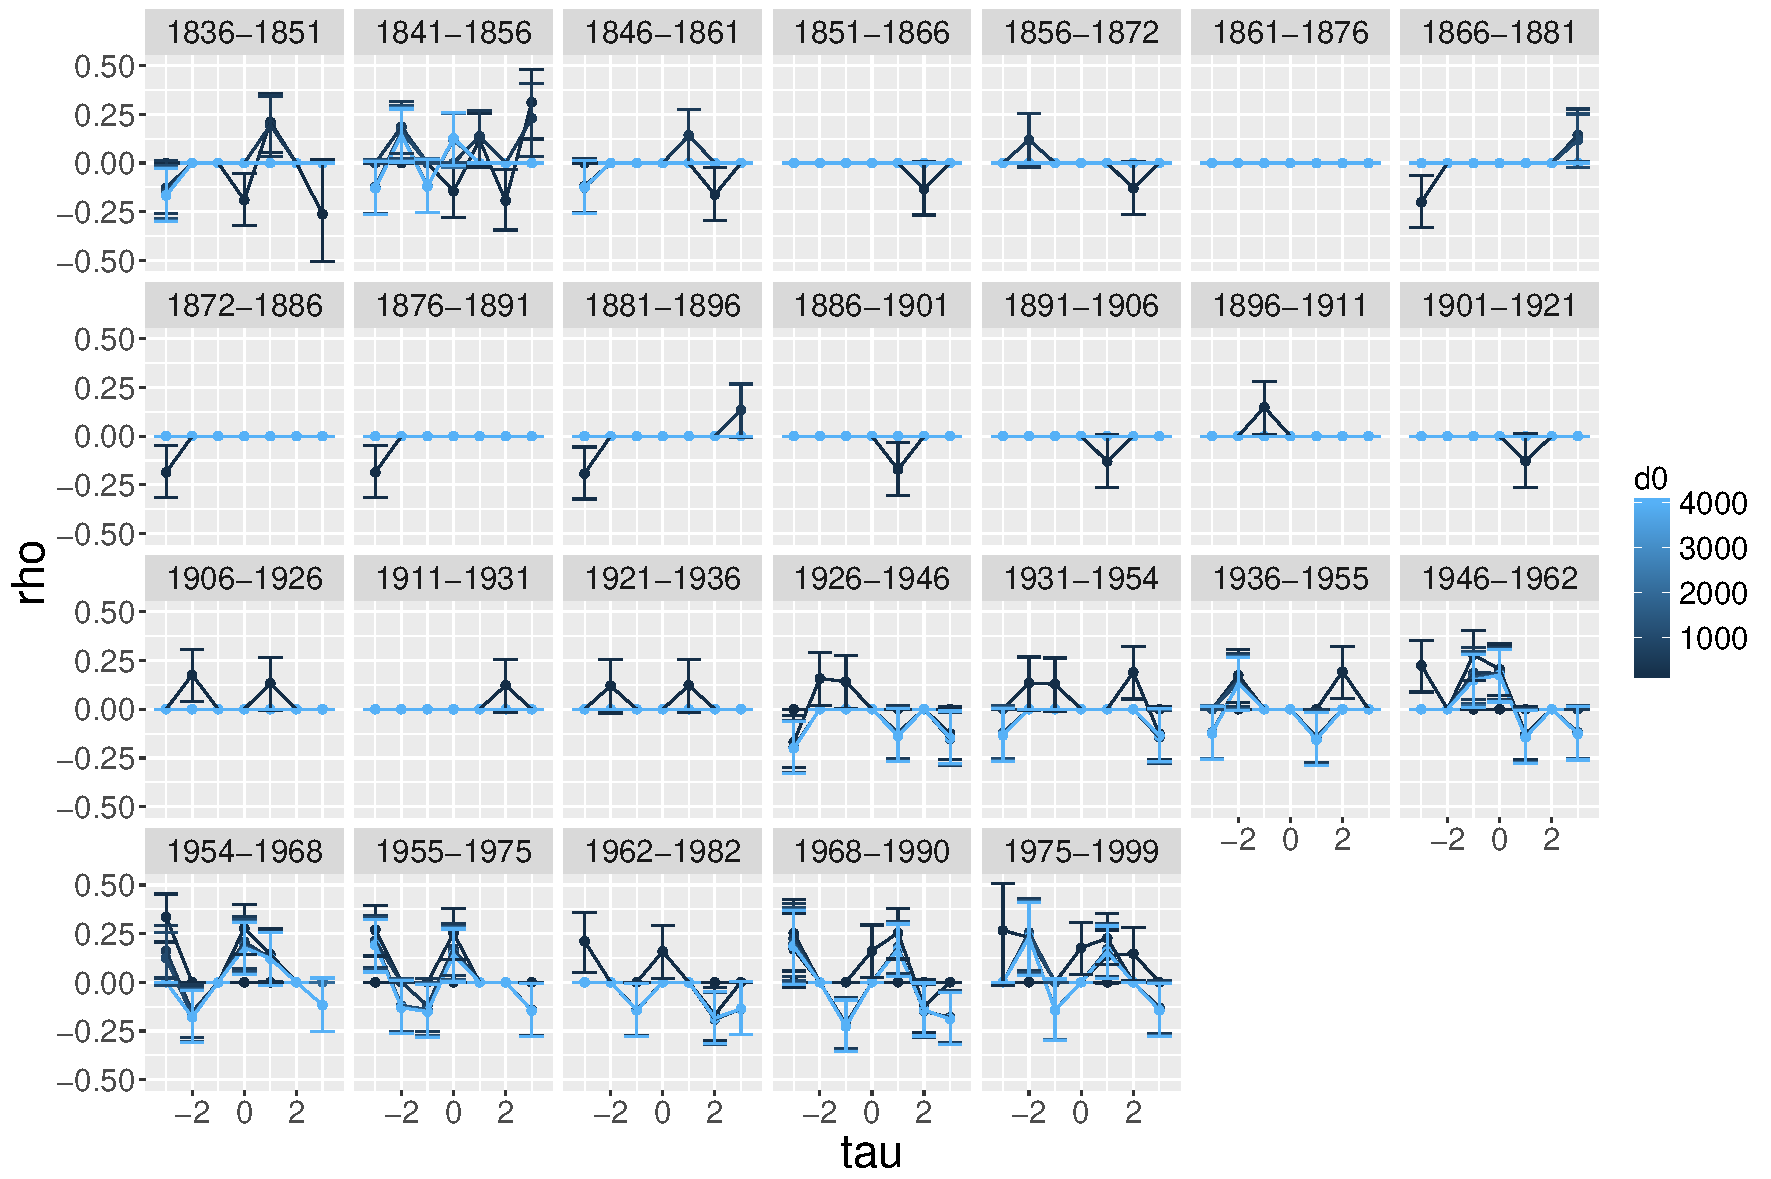
\includegraphics[width=\linewidth]{Figures/MacroCoEvol/laggedCorrs_time_Tw4.pdf}
	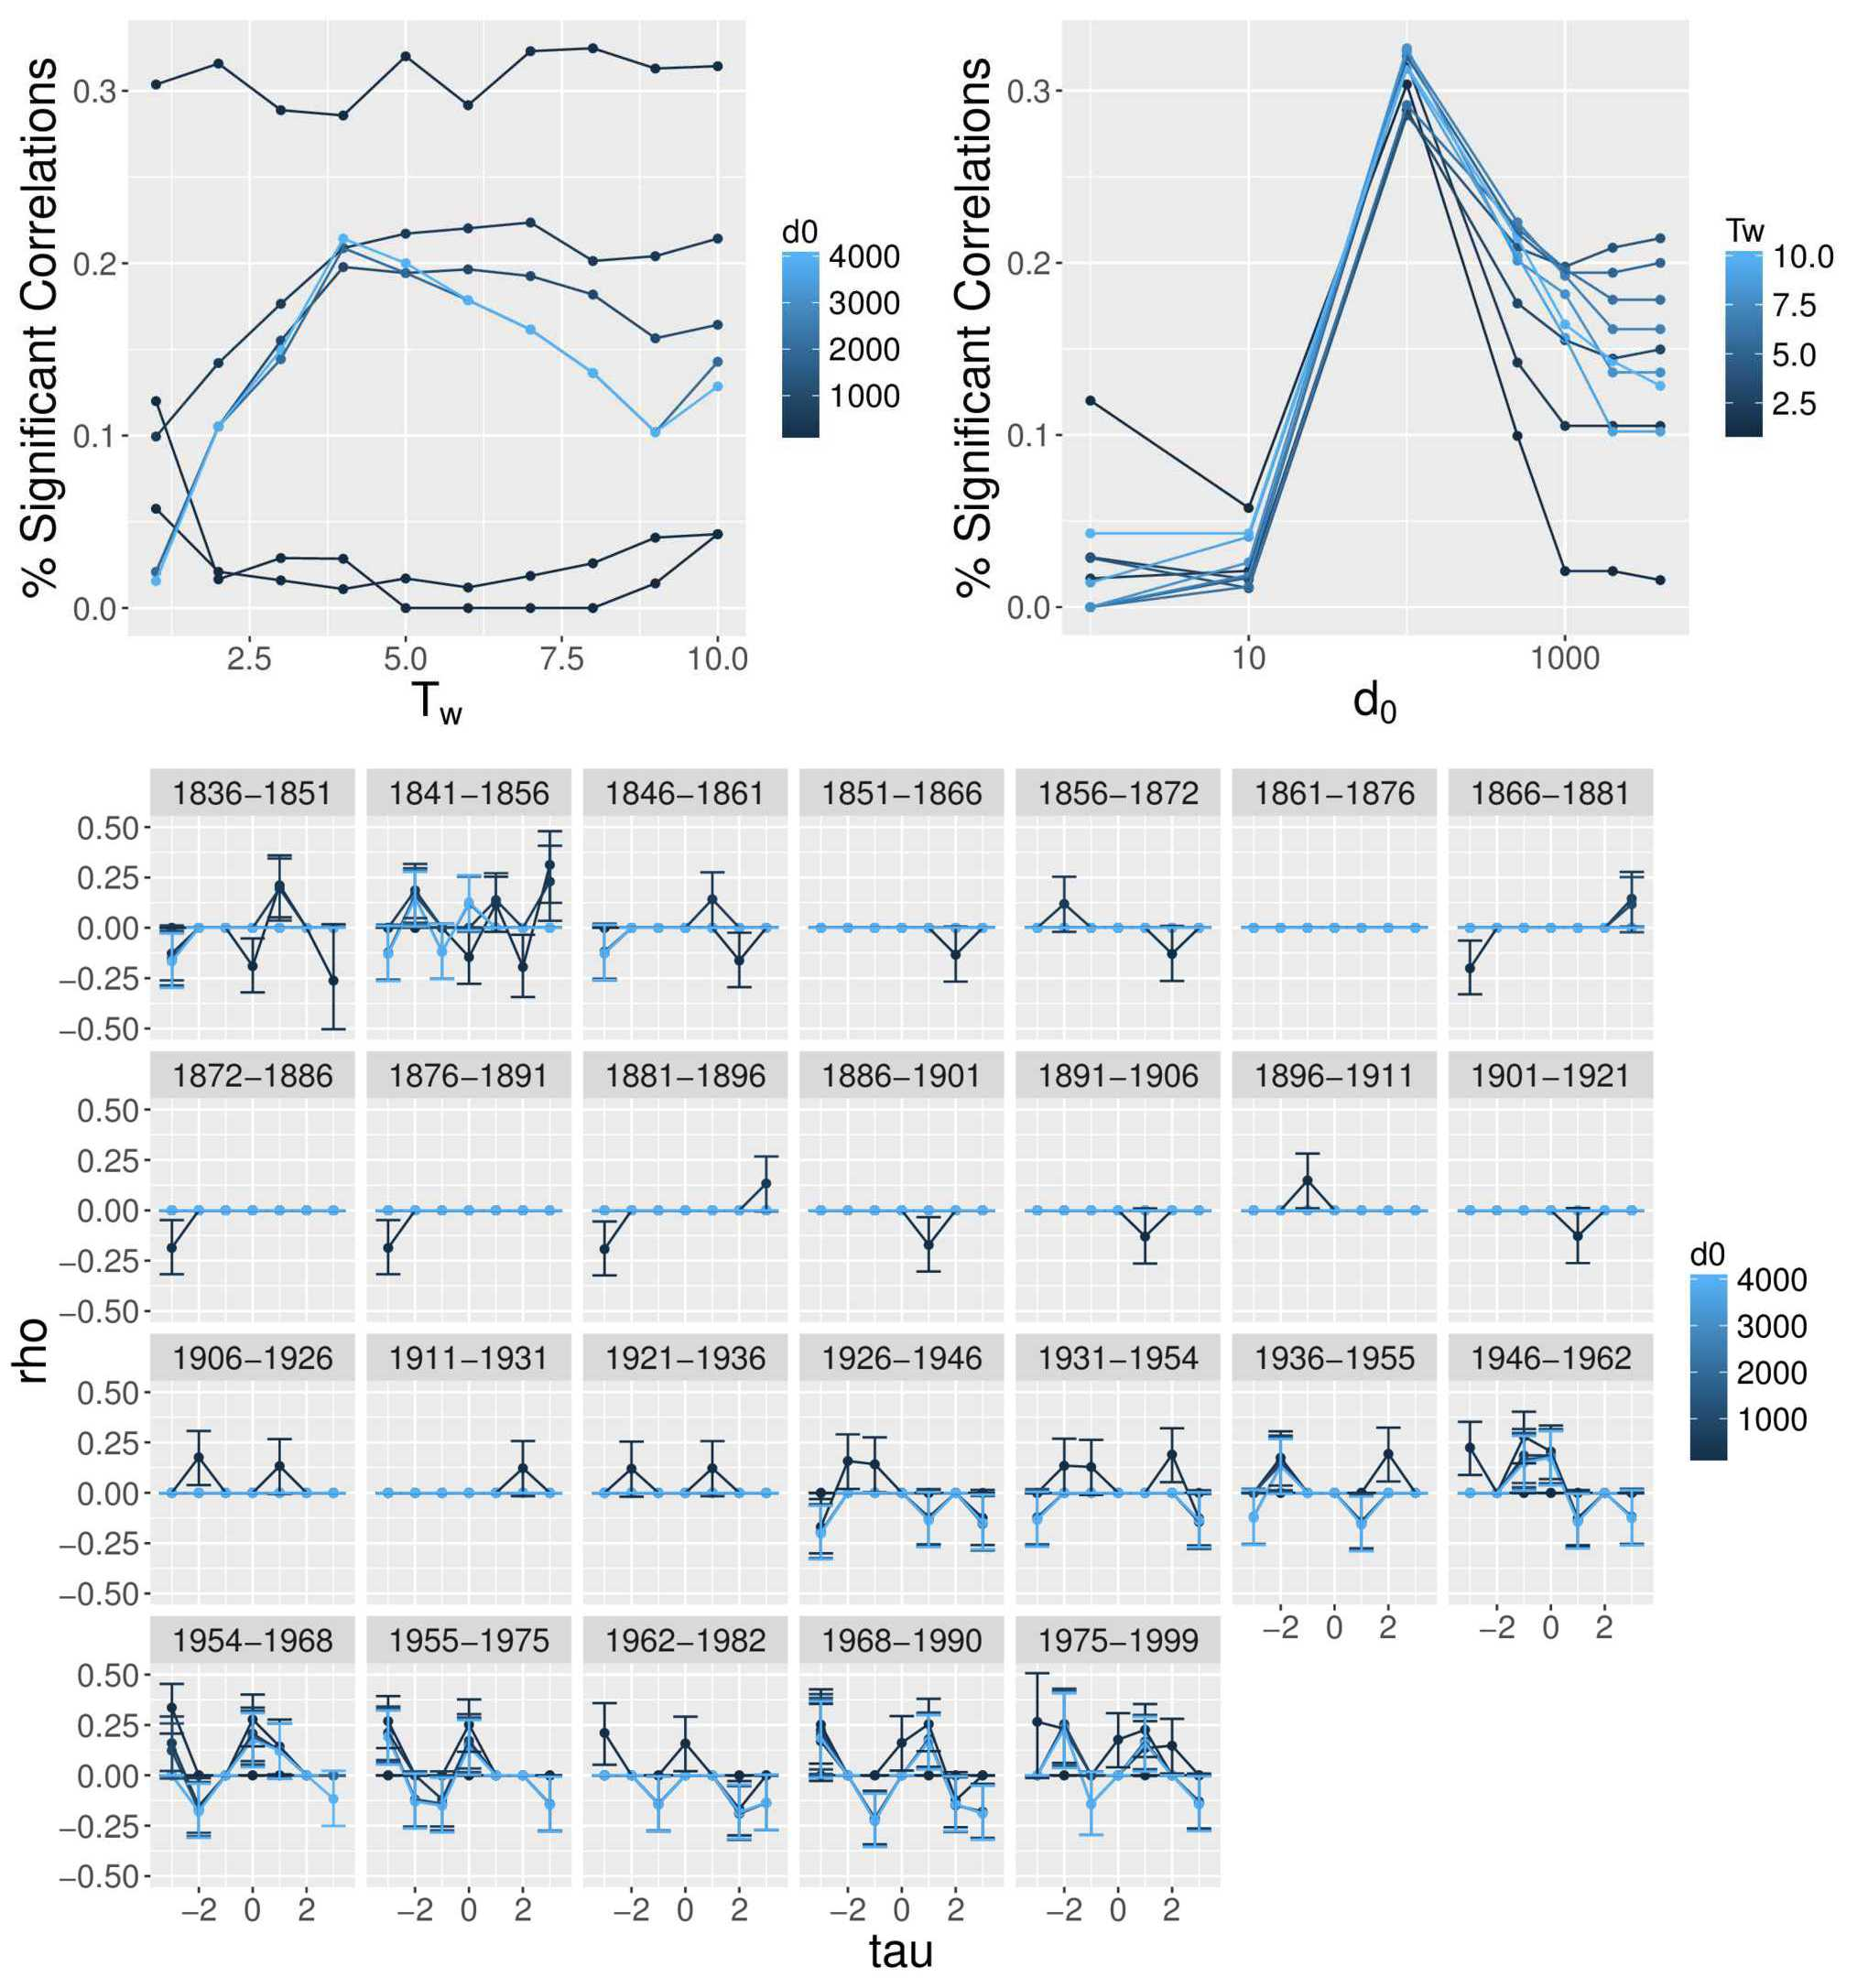
\includegraphics[width=\linewidth]{Figures/Final/6-2-3-fig-macrocoevol-empirical.jpg}
	\caption[Empirical Lagged Correlations for French City System][Corrélations empiriques pour le système de villes français]{\label{fig:macrocoevol:empirical}}{\textbf{Corrélations retardées empiriques pour le système de villes français.} Les corrélations sont calculées sur une fenêtre de taille $5\cdot T_w$, entre les taux de croissance des populations et ceux de centralité de proximité avec un paramètre de décroissance $d_0$ (voir texte). \textit{(Haut Gauche)} Nombre de corrélation significatives (prises telles que $p<0.1$ à 95\%) en fonction de $T_w$ pour $d_0$ variable ; \textit{(Haut droite)} Nombre de corrélations significatives en fonction de $d_0$ pour $T_w$ variable ; \textit{(Bas)} Pour la fenêtre ``optimale'' $T_w=4$, valeur de $\rho_{\tau}$ en fonction de $\tau$, pour l'ensemble des périodes successives.\comment[AB]{graphes plus ciblés (?)}\label{fig:macrocoevol:empirical}}
\end{figure}
%%%%%%%%%%%%%









\subsubsection{Abstract model calibration}{Calibration du modèle abstrait}


\bpar{
Expected results concern both accurate city population growth reproduction, and network patterns, i.e. how does taking into account dynamical networks can introduce further exploratory power in such models for population trajectories, and also how realistic network distance evolution is.
}{
Les résultats attendus de la calibration sur données réelles concernent à la fois la reproduction plus ou moins précise des dynamiques réelles de croissance de population, c'est à dire dans quelle mesure la prise en compte d'un réseau dynamique peut augmenter le pouvoir explicatif pour les trajectoires, et aussi quel est le niveau de réalisme de l'évolution de la distance par le réseau. Nous travaillons toujours avec le modèle abstrait.
}


\paragraph{Indicators}{Indicateurs}\comment[FL]{plutot : mesure de performance des ecarts aux observations}

On peut ajouter aux indicateurs utilisés précédemment un indicateur de calibration pour la distance. L'aspect particulier de l'ajustement pour les populations, qui résidait dans la présence d'une loi de puissance pour les tailles de villes rendant négligeables les performances sur les villes moyennes et les petites villes dans le cas d'une erreur cumulée, et suggérait l'ajout de l'indicateur de l'erreur sur les logarithmes\comment[FL]{detail technique a ce stade ?}, n'est pas présent pour les distances qui suivent une distribution concentrée sur un ordre de grandeur unique. Nous utilisons ainsi le logarithme de l'erreur carré sur les distances, donnée par\comment[FL]{cela ne donne pas plus d'eclairage sur tes choix}

\[
\varepsilon_D = \log \left[ \sum_t \sum_{i,j} \left(d_{ij}(t) - \tilde{d}_{ij}(t)\right)^2\right]
\]

\comment[AB]{preciser + references}




%%%%%%%%%%%%%
%% ON HOLD : benchmark static model with real network distances


%\paragraph{Role of Real Network Distances}{Rôles des distances réelles de réseau}

%\bpar{
%We use as a benchmark network the geographical shortest paths that have been shown in a previous work to already capture network effects (see~\cite{raimbault2016models} and section~\ref{sec:interactiongibrat}).
%}{
%Nous utilisons comme réseau de benchmark les plus courts chemins géographiques qui ont été montrés déjà capturer des effets de réseaux dans un précédent travail (voir~\cite{raimbault2016models} et la section~\ref{sec:interactiongibrat}).
%}




\paragraph{Results}{Résultats}


Nous procédons à une calibration non-stationnaire, sur les objectifs $(\varepsilon_P,\varepsilon_D)$\comment[FL]{expliciter}, par fenêtre mobile sur les périodes déjà utilisées en~\ref{sec:interactiongibrat}. Pour limiter la dimension à explorer, nous fixons $w_N = 0$ pour n'étudier les interactions qu'au premier ordre, sachant que les paramètres de réseau abstrait $(g_{max},\gamma_S,\varphi_0)$ sont pris en compte dans la calibration. La calibration est effectuée par algorithme génétique de façon similaire La Fig.~\ref{fig:macrocoevol:pareto} montre les fronts de Pareto obtenus, et la Fig.~\ref{fig:macrocoevol:parameters} l'évolution dans le temps des valeurs des paramètres pour les solution optimales. On note la faible consistence des fronts de Pareto de manière générale, en comparaison avec ceux obtenus pour la population seule précédemment, ce qui suggère la difficulté d'optimiser conjointement trajectoire des populations et trajectoire des distances. Certaines périodes, comme 1851-1872 puis toutes celles après 1946, présentent un point optimal simultané pour les deux objectifs, ce qui pourrait aussi témoigner d'une mauvaise convergence de l'algorithme. Dans tous les cas, la très faible significativité des corrélations empiriques observées précédemment pouvait laisser présager de ces mauvais ajustements. Les valeurs des paramètres optimaux semblent toutefois contenir un certain signal. L'évolution de $w_G$ et $\gamma_G$ sont consistantes avec celles observées pour le modèle statique. Pour $d_G$, on observe des oscillations, une certaine stabilité, puis un pic pour la période 1962-1982. Il pourrait s'agir d'un ``effet TGV'', en cohérence avec le pic secondaire pour $\phi_0$ observé au même point, puisque la construction des LGV a raccourci les distances entre les villes au plus haut de la hiérarchie (une augmentation du seuil $\phi_0$ correspond à une augmentation de la sélectivité pour une diminution potentielle des distances). Le $g_{max}$ calibré est très représentatif de l'histoire du réseau ferré : un très fort accroissement dans les premières années, puis un accroissement stable plus tard (l'impact du TGV étant là noyé dans l'ensemble du réseau, le seul signe étant une augmentation de la déviation sur l'ensemble du front). Pour la calibration avec distance seule, la stabilisation à $g_{max}=0$ est un témoin de la rudimentarité du modèle. On a pu ainsi dans une certaine mesure indirectement quantifier les processus d'interaction par le réseau et ceux d'adaptation du réseau au flux, dans le cas d'un système réel.\comment[FL]{discussion interessante}

%%%%%%%%%%%%%%%%%%%
\begin{figure}
	%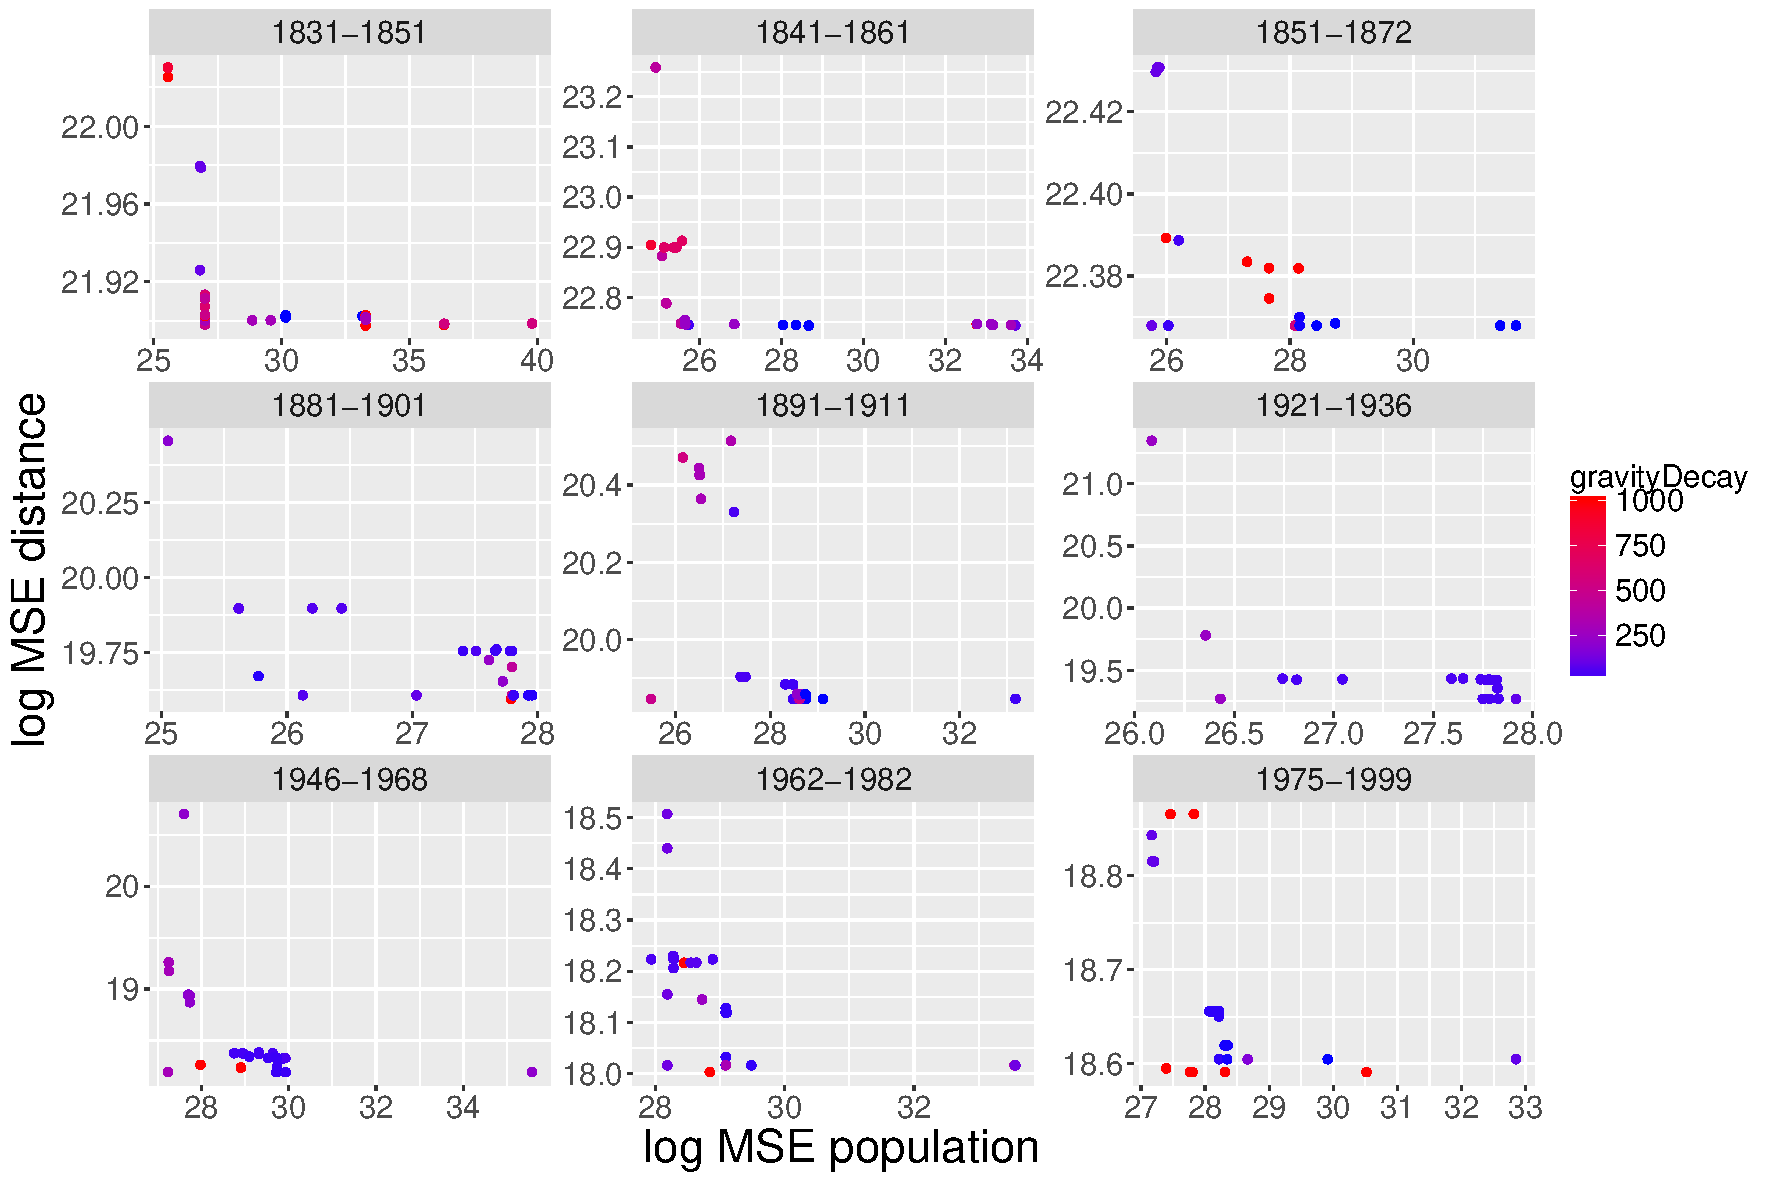
\includegraphics[width=0.9\linewidth]{Figures/MacroCoEvol/pareto_gravityDecay}\\
	%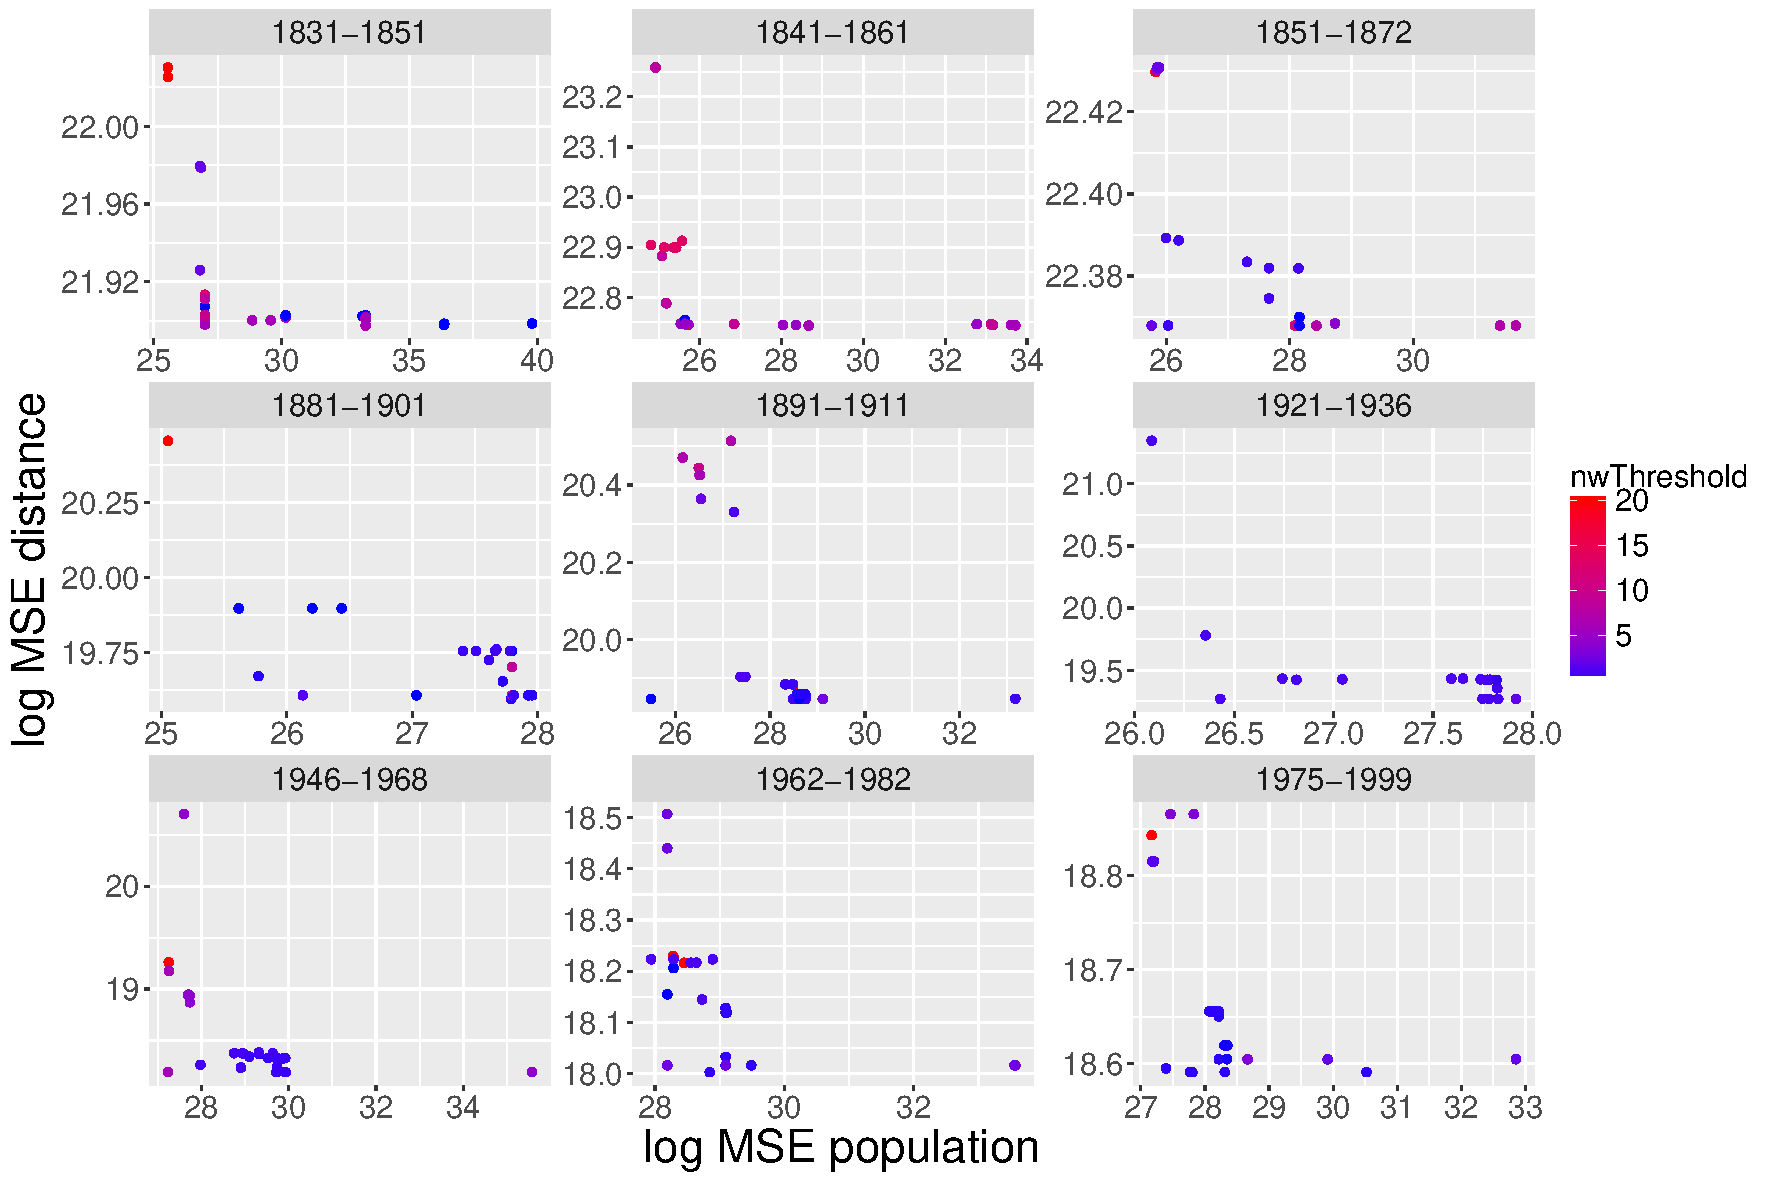
\includegraphics[width=0.9\linewidth]{Figures/MacroCoEvol/pareto_nwThreshold}
	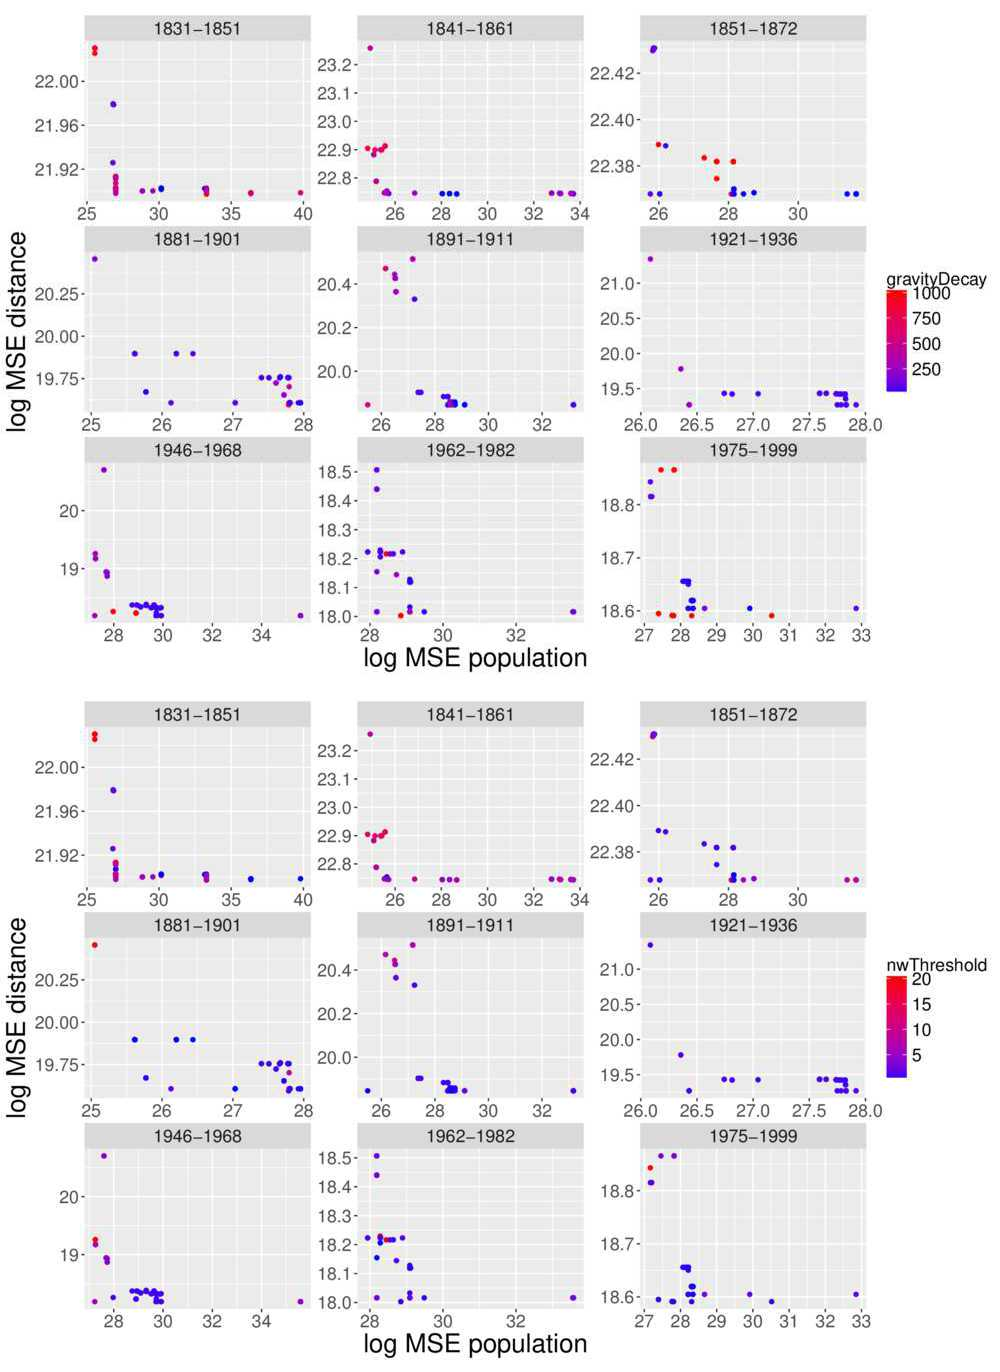
\includegraphics[width=\linewidth,height=0.9\textheight]{Figures/Final/6-2-3-fig-macrocoevol-pareto}
	\caption[Pareto fronts][Fronts de Pareto]{\label{fig:macrocoevol:pareto}}{\textbf{Fronts de Pareto pour la calibration bi-objectif population et distance.} Les fronts sont donnés pour chaque période de calibration, et colorés en fonction de $d_G$ (Haut) et de $\phi_0$ (Bas).\comment[FL]{()}\label{fig:macrocoevol:pareto}}
\end{figure}
%%%%%%%%%%%%%%%%%%%


%%%%%%%%%%%%%%%%%%%
\begin{figure}
	%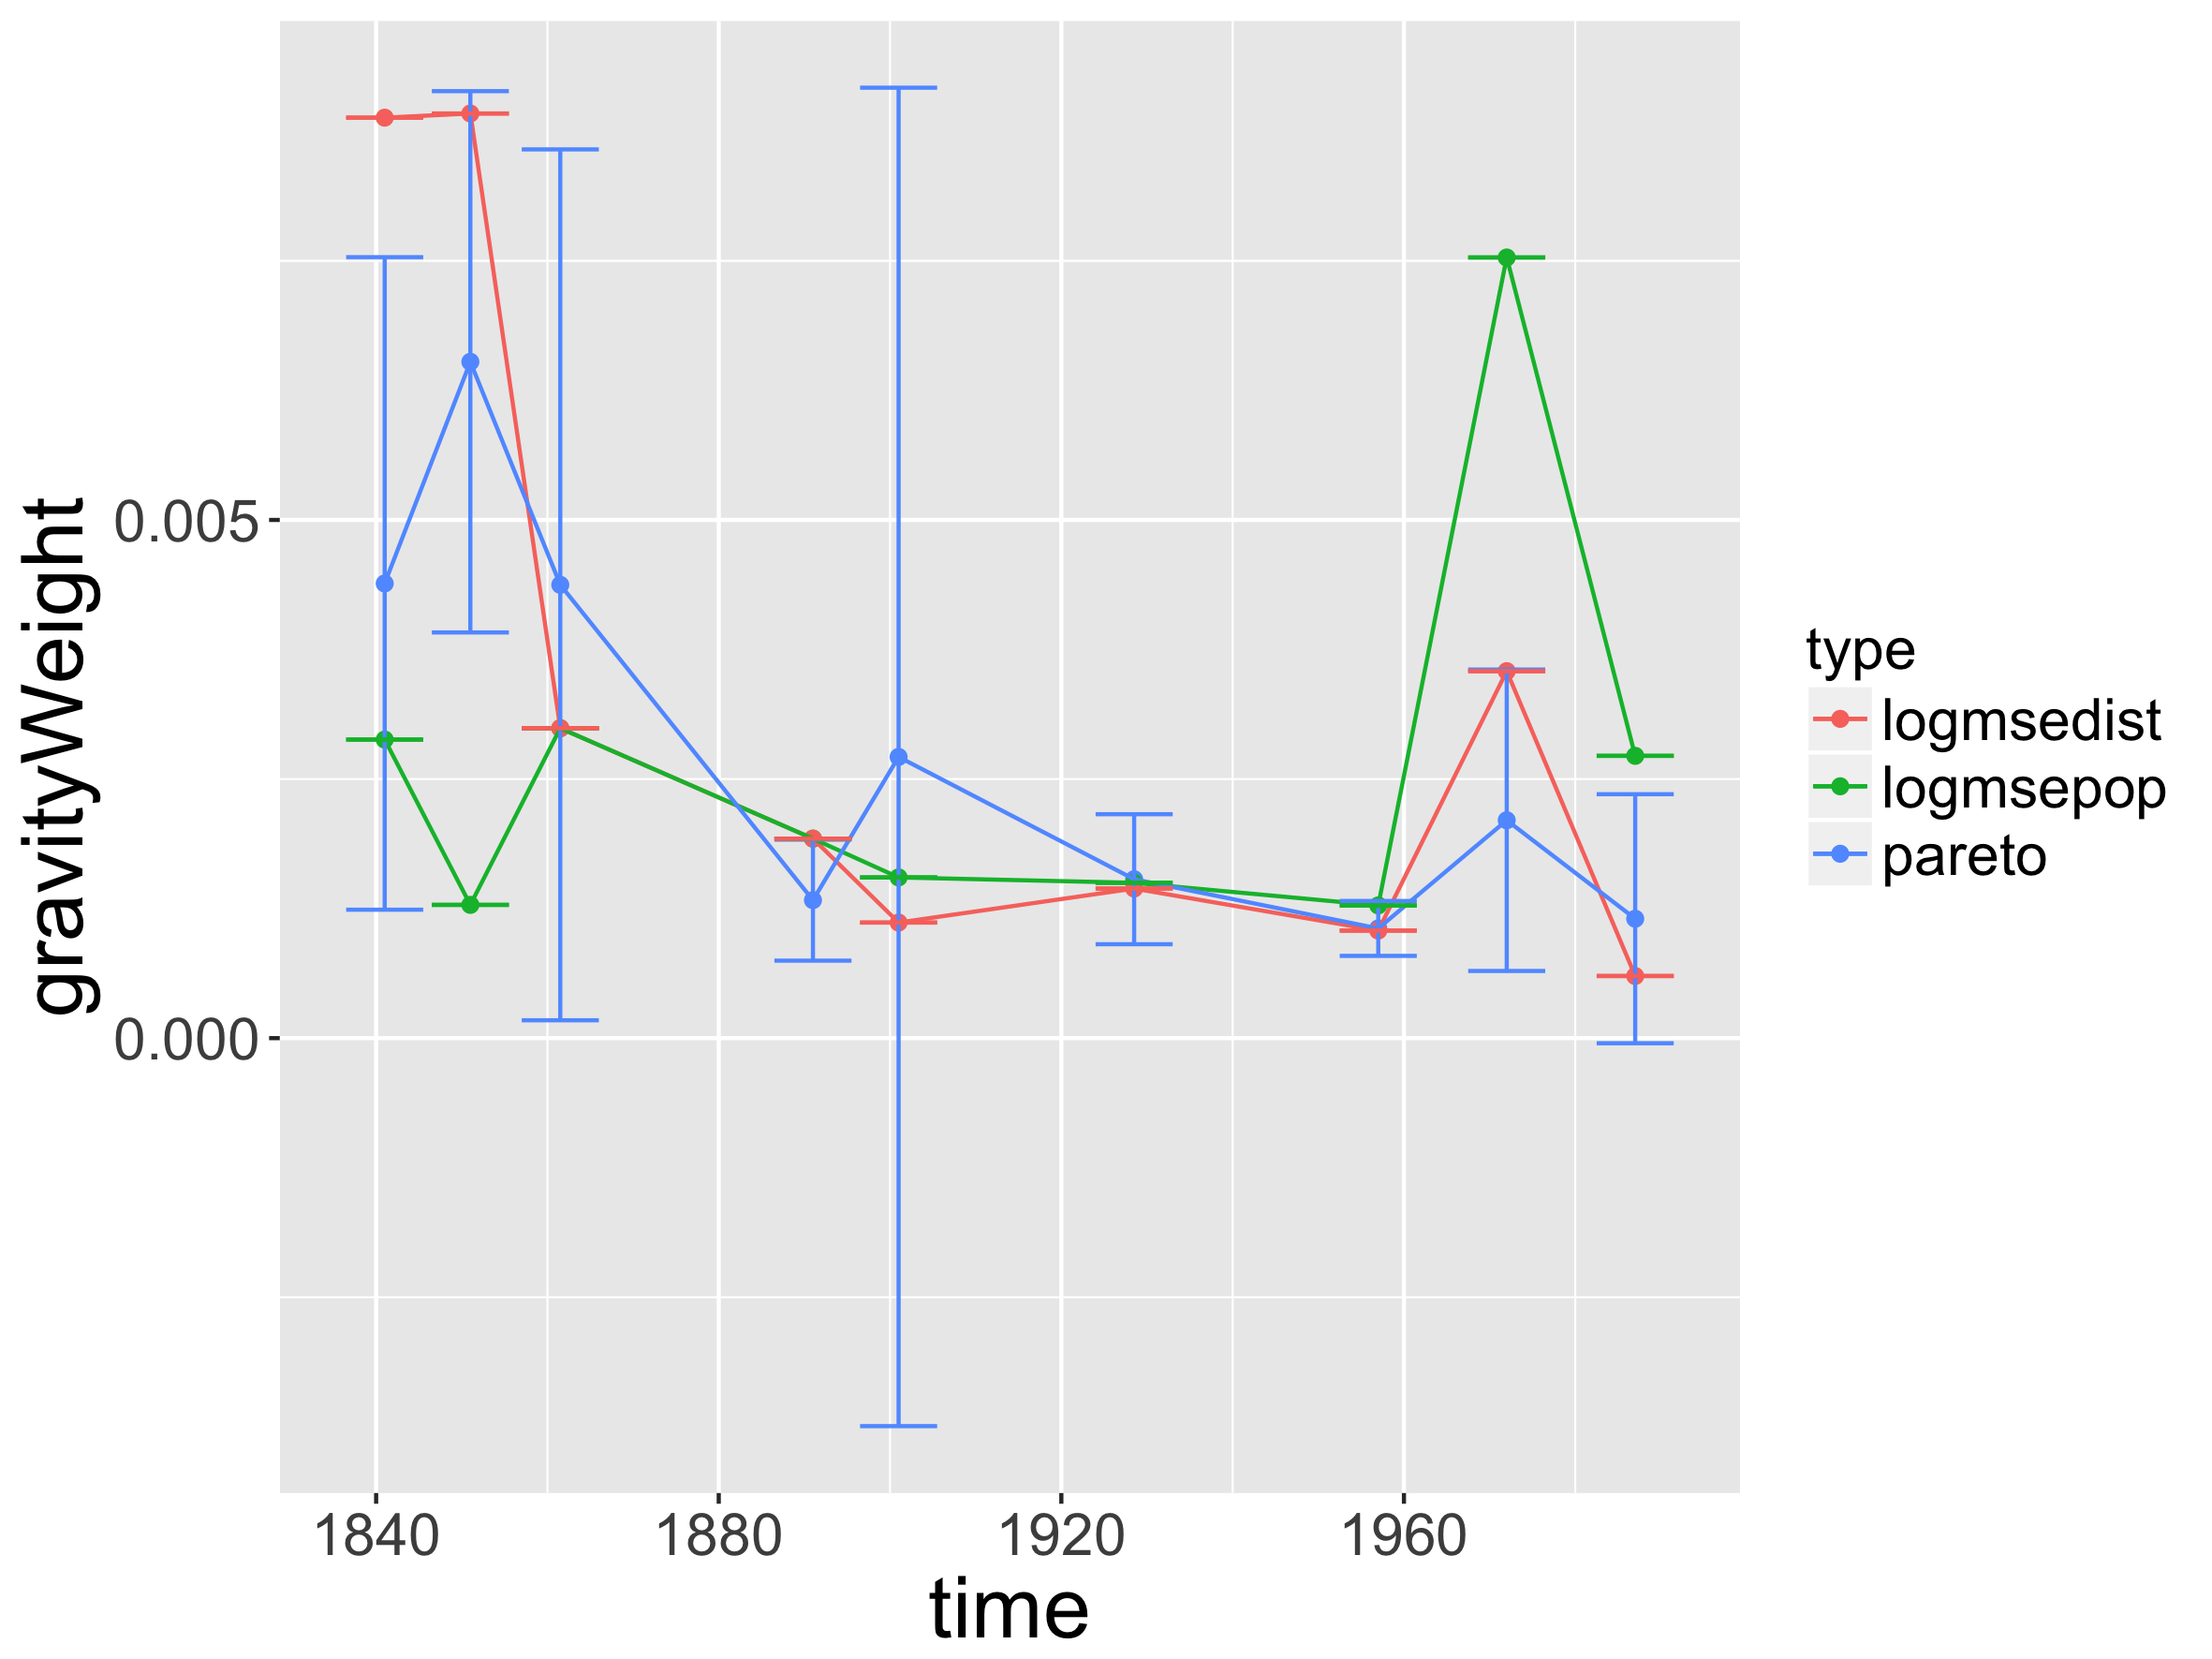
\includegraphics[width=0.32\linewidth]{Figures/MacroCoEvol/param_gravityWeight_filt1}
	%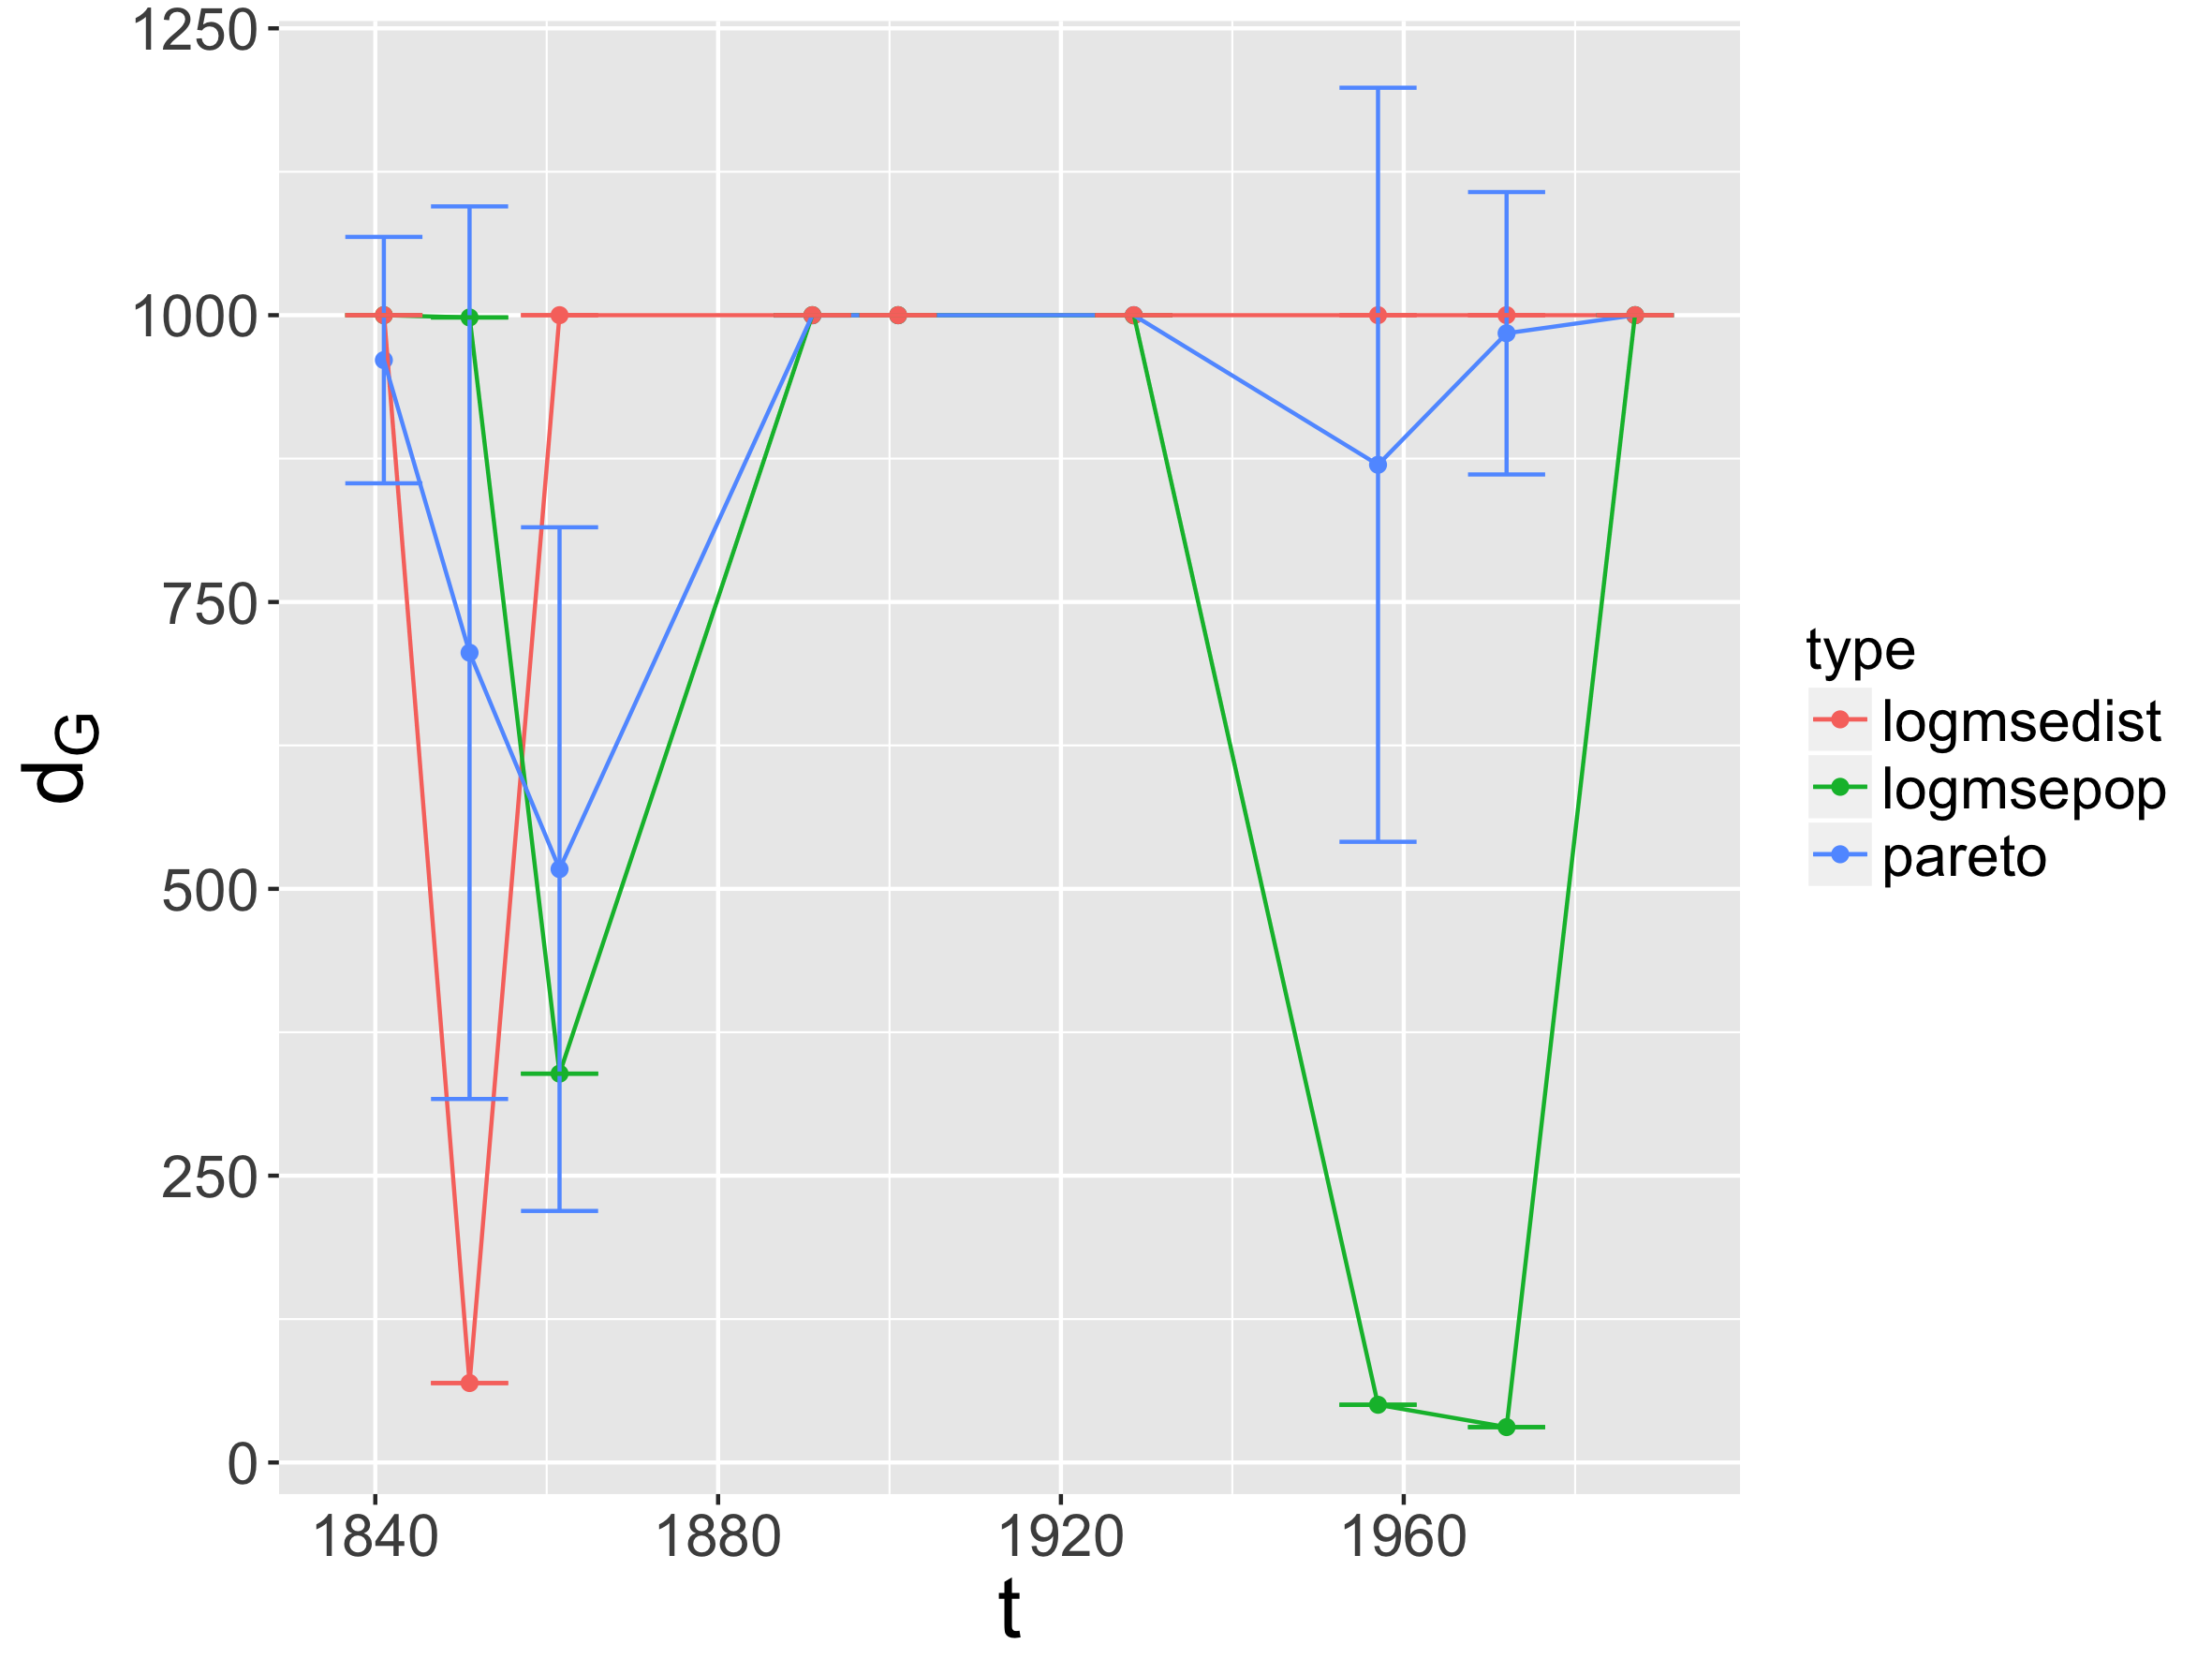
\includegraphics[width=0.32\linewidth]{Figures/MacroCoEvol/param_gravityDecay_filt1}
	%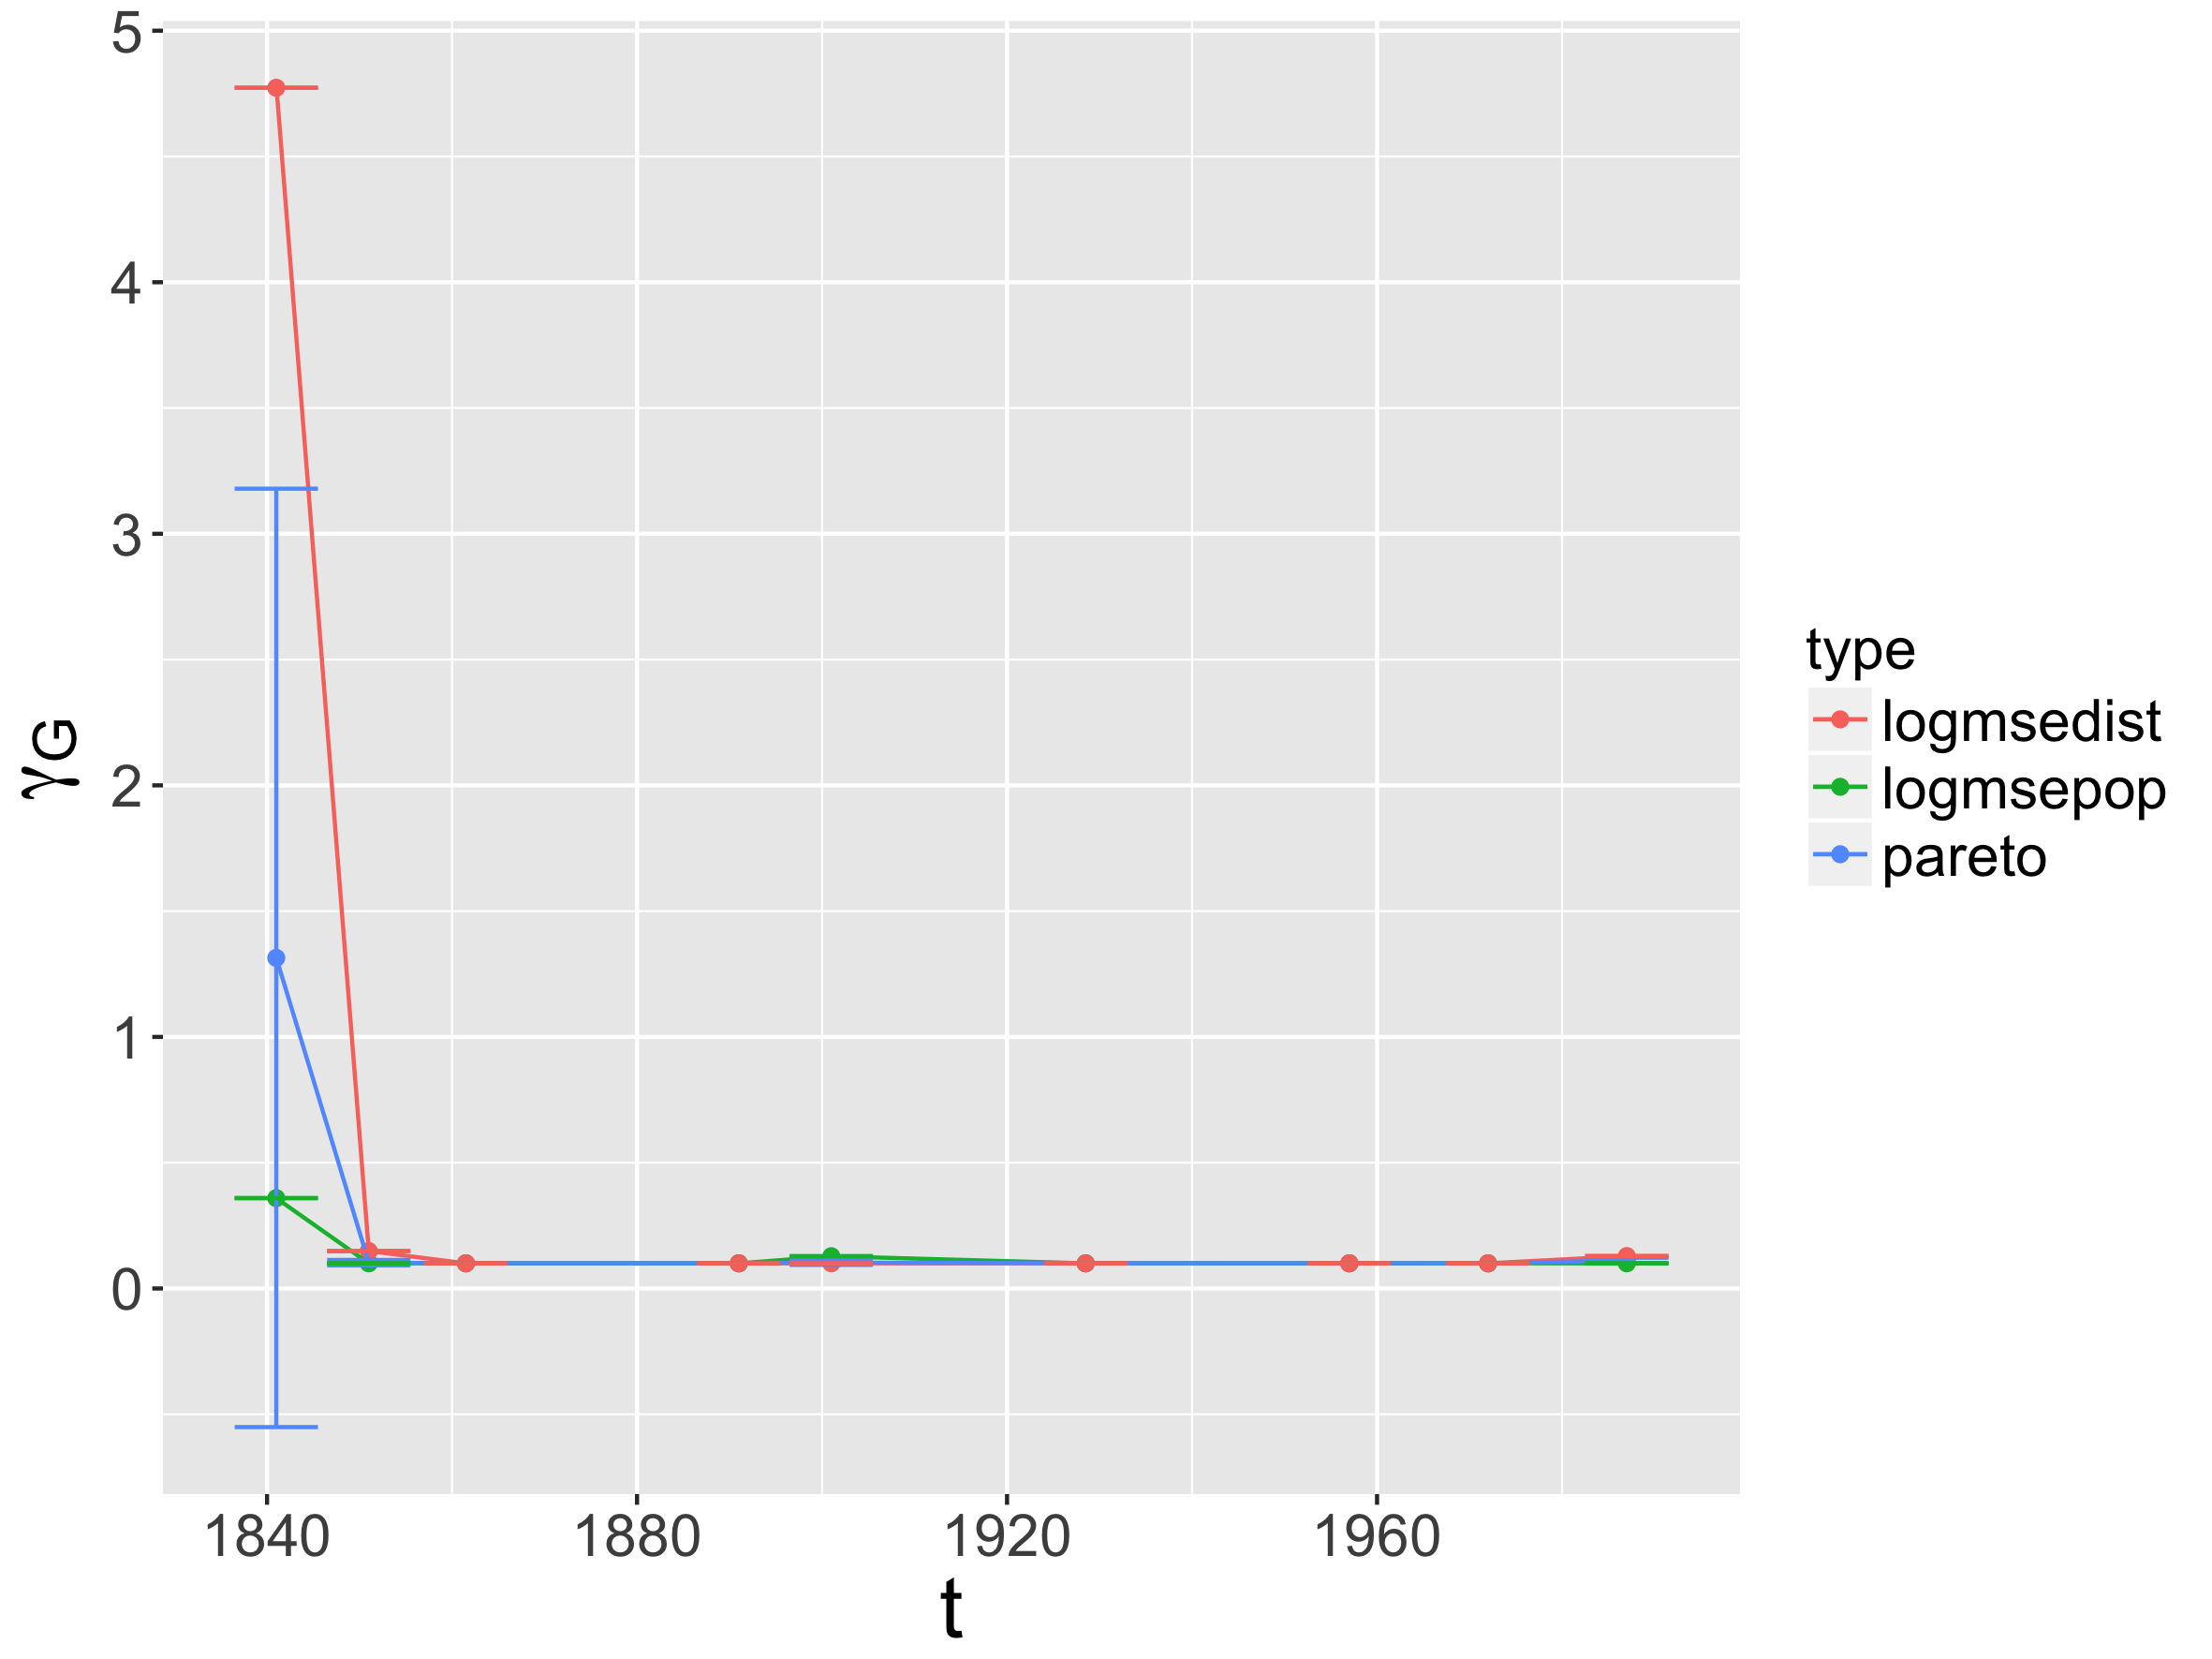
\includegraphics[width=0.32\linewidth]{Figures/MacroCoEvol/param_gravityGamma_filt1}\\
	%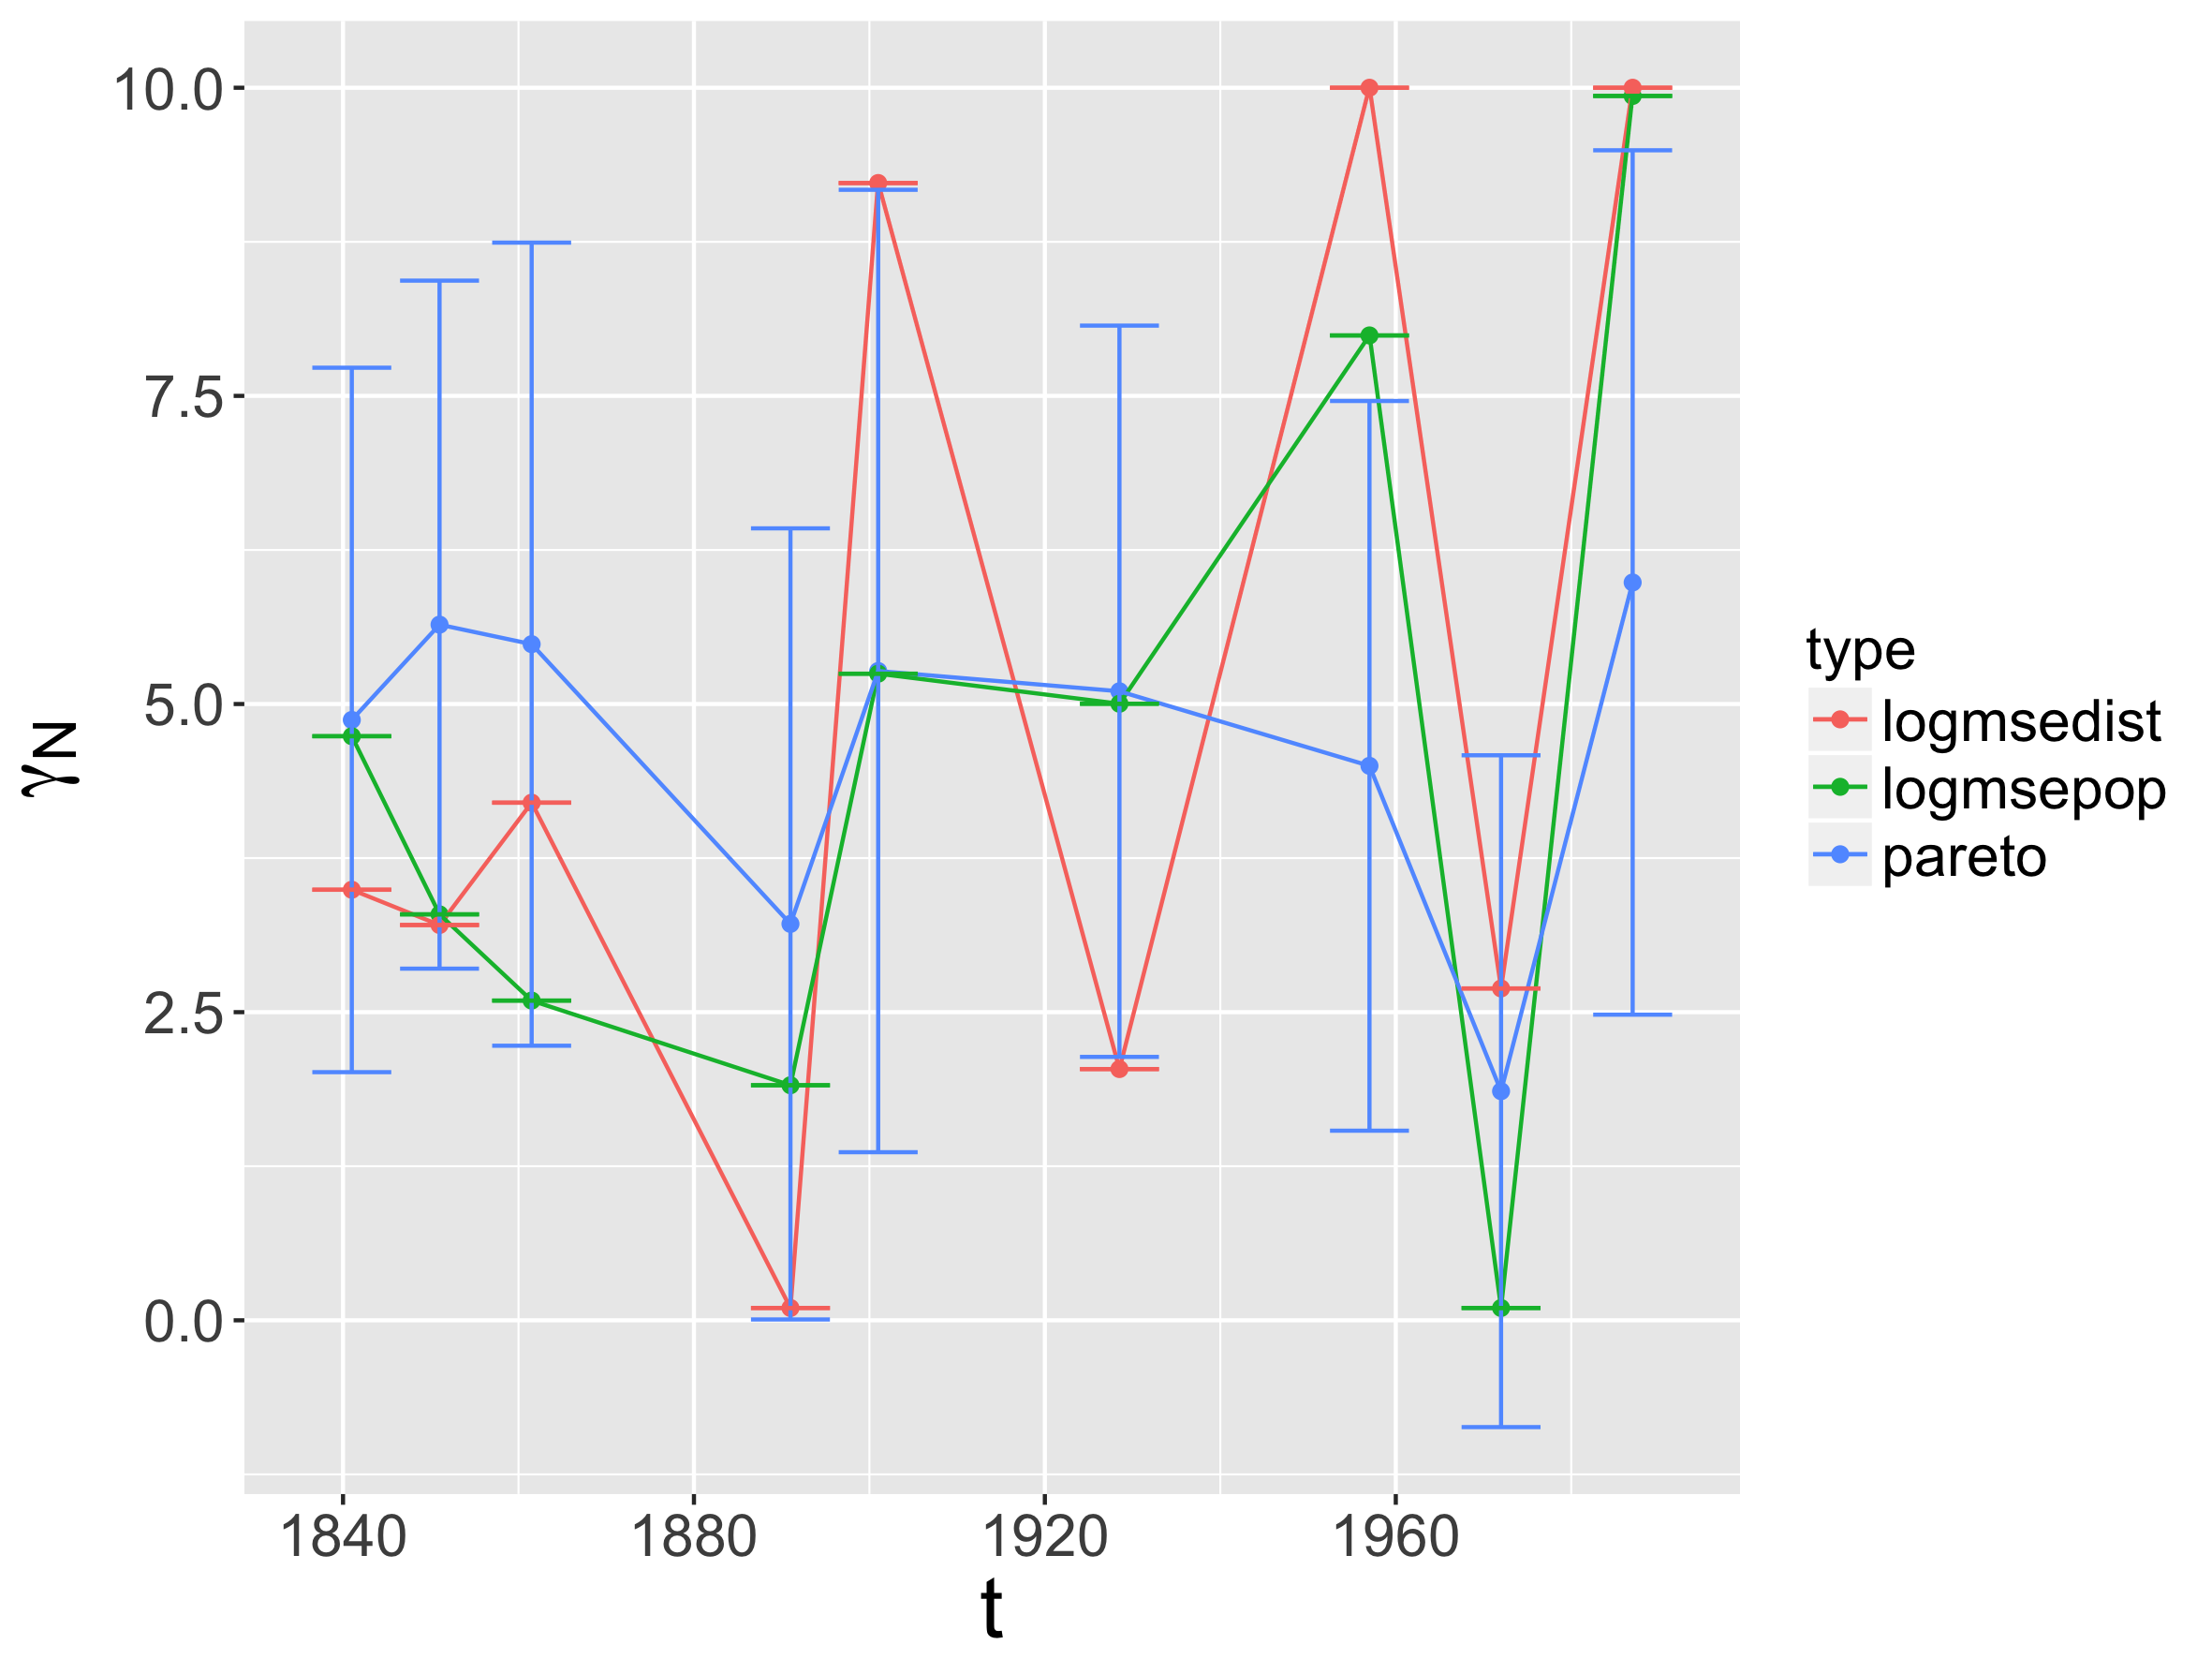
\includegraphics[width=0.32\linewidth]{Figures/MacroCoEvol/param_nwExponent_filt1}
	%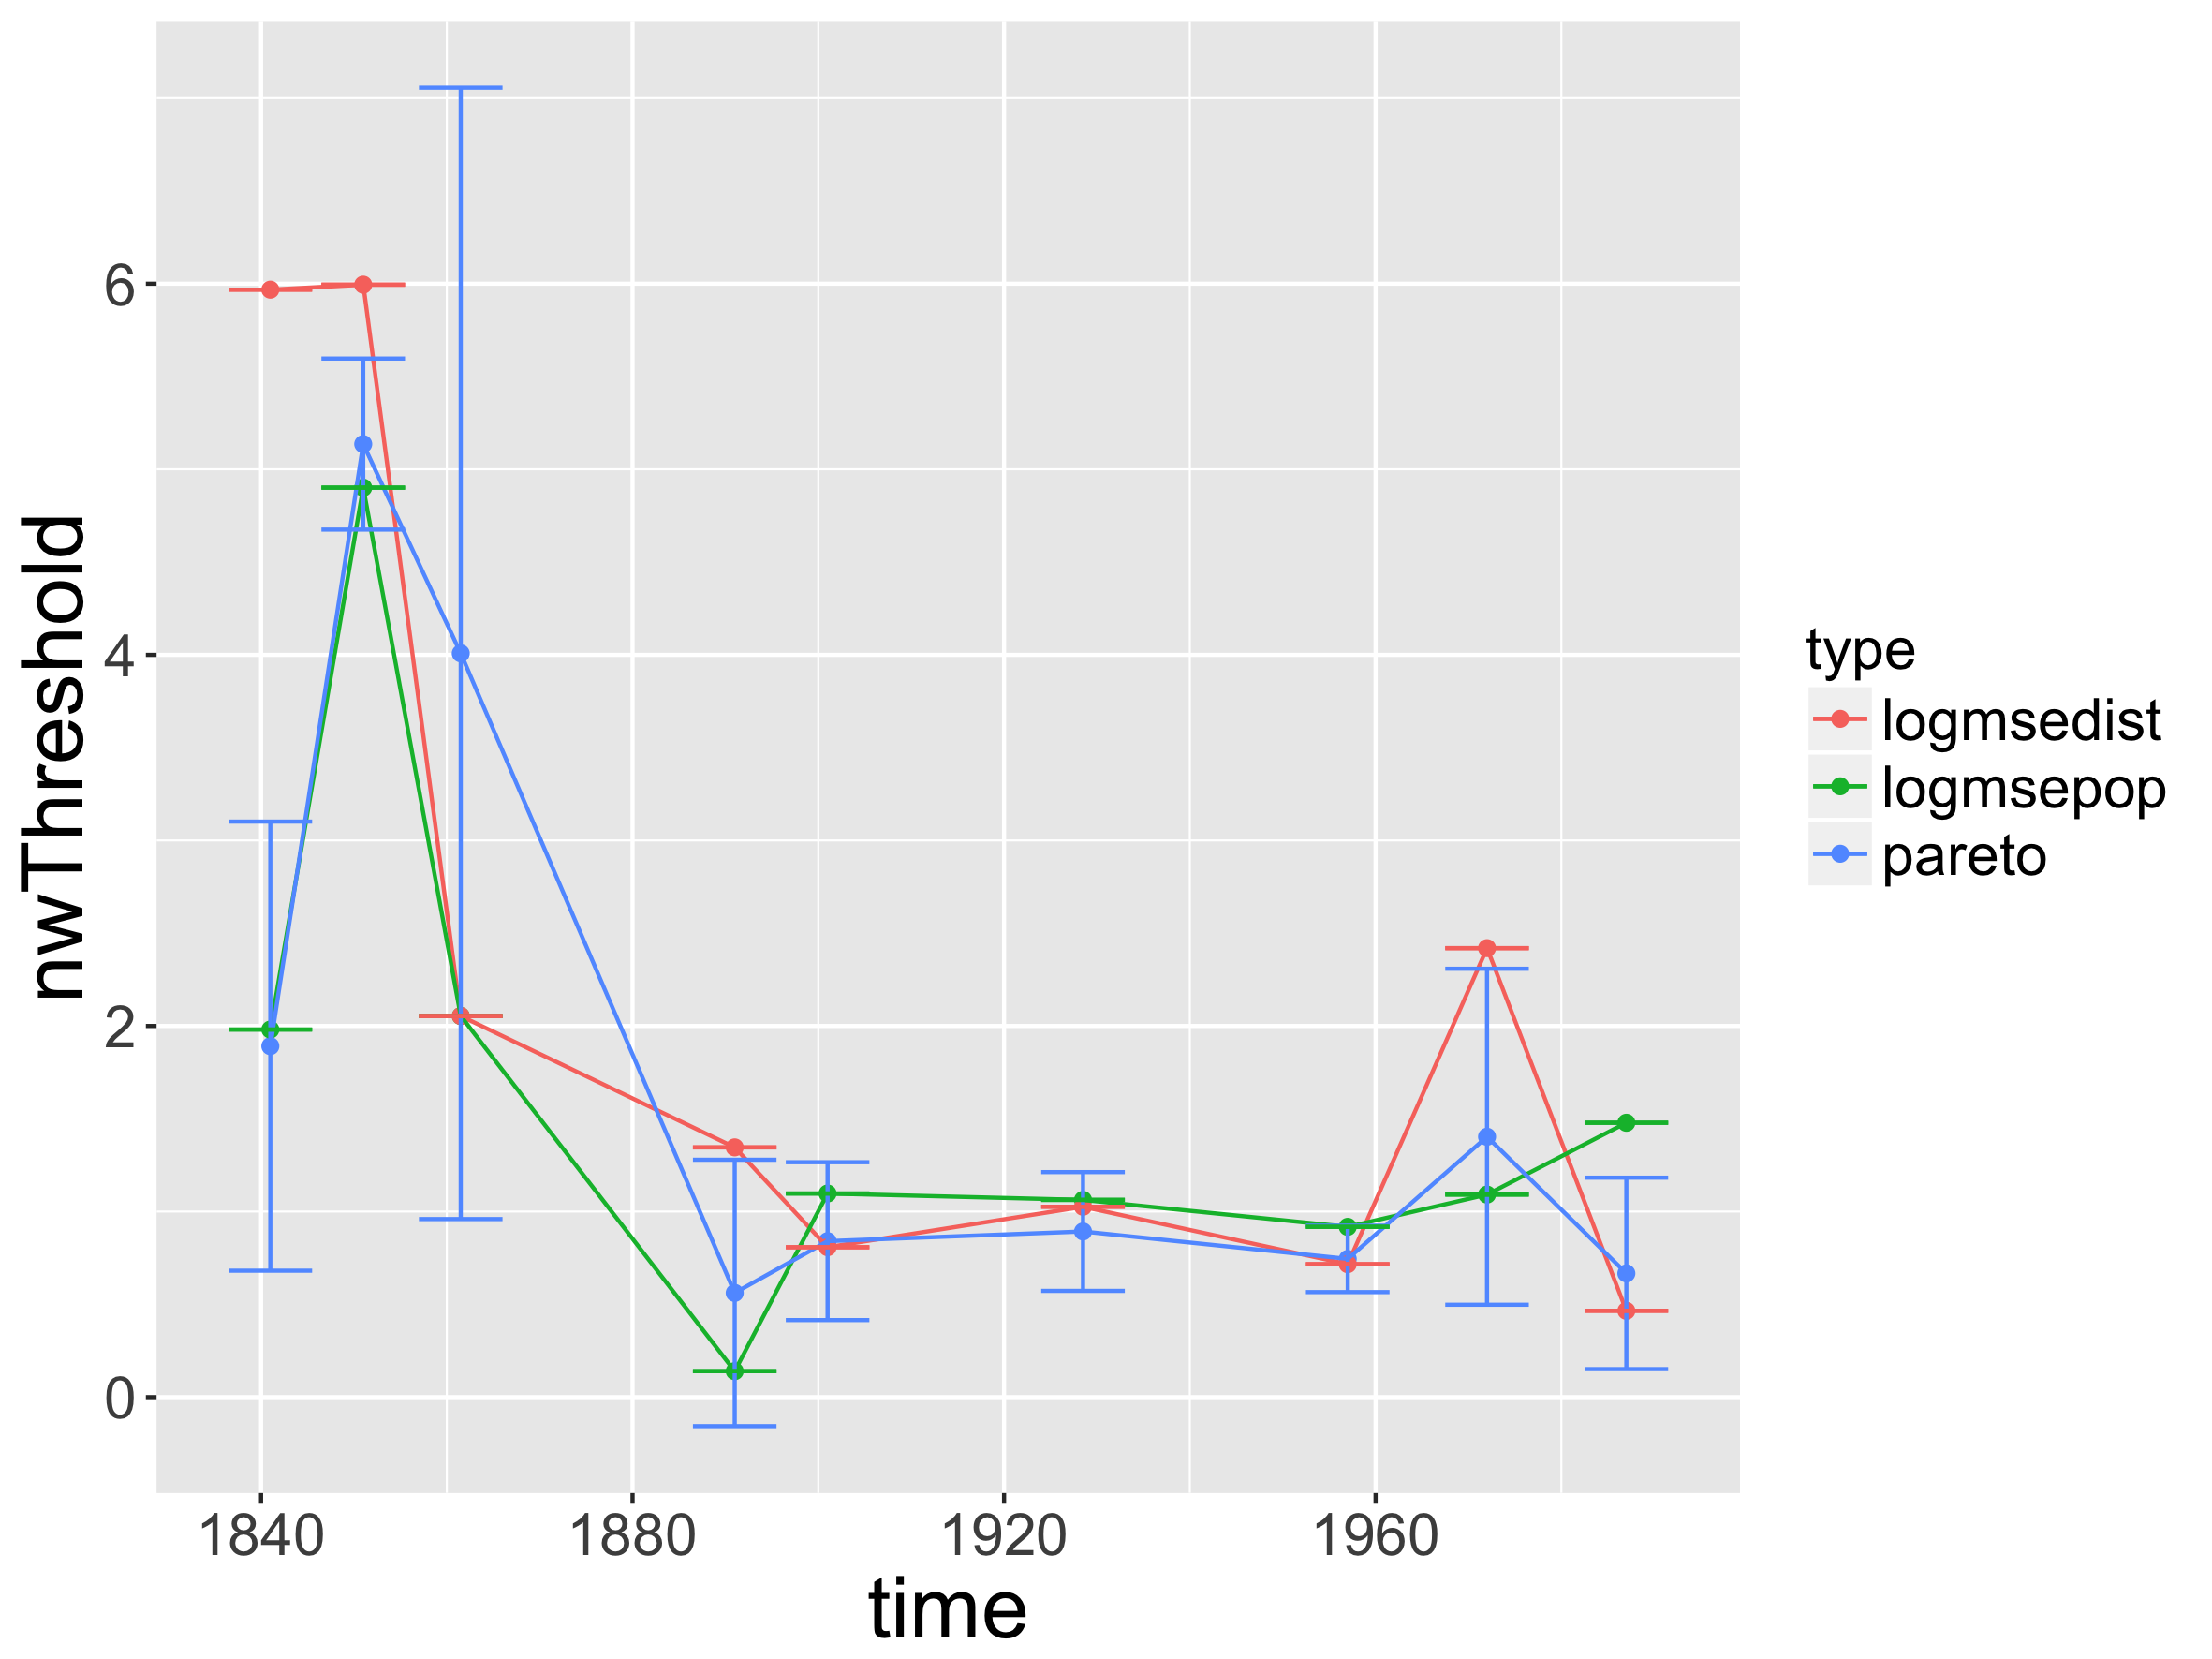
\includegraphics[width=0.32\linewidth]{Figures/MacroCoEvol/param_nwThreshold_filt1}
	%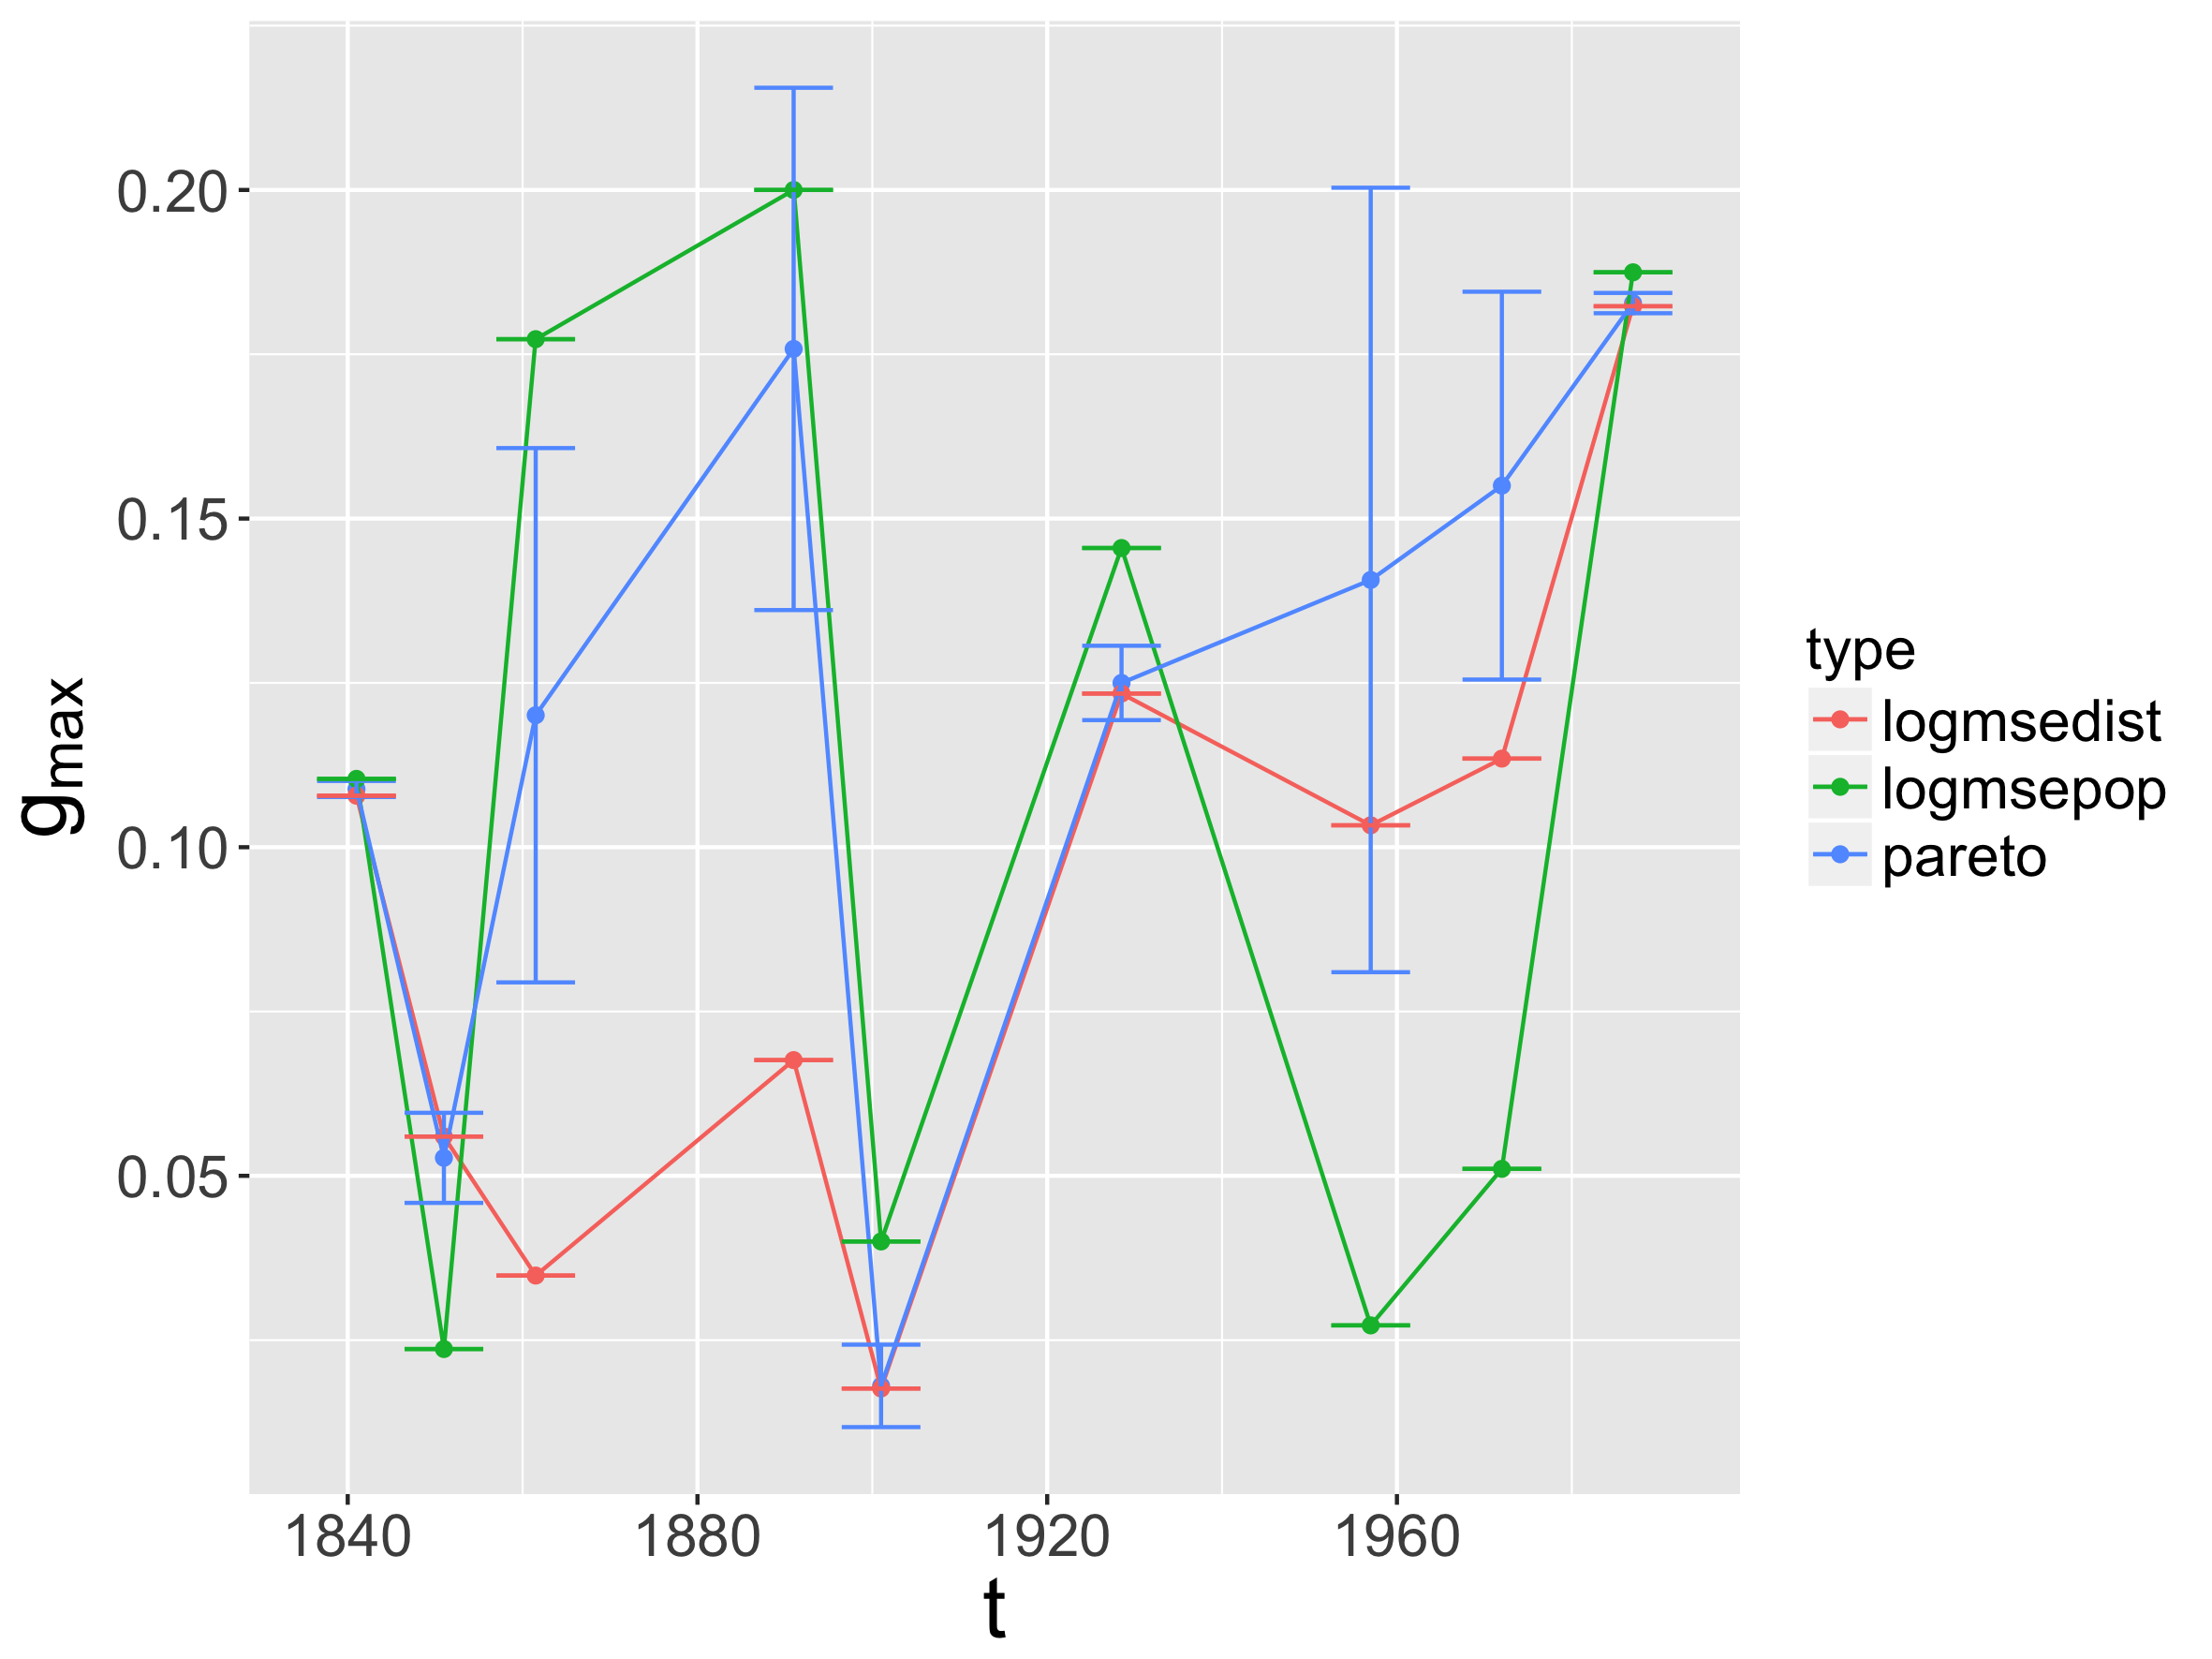
\includegraphics[width=0.32\linewidth]{Figures/MacroCoEvol/param_nwGmax_filt1}
	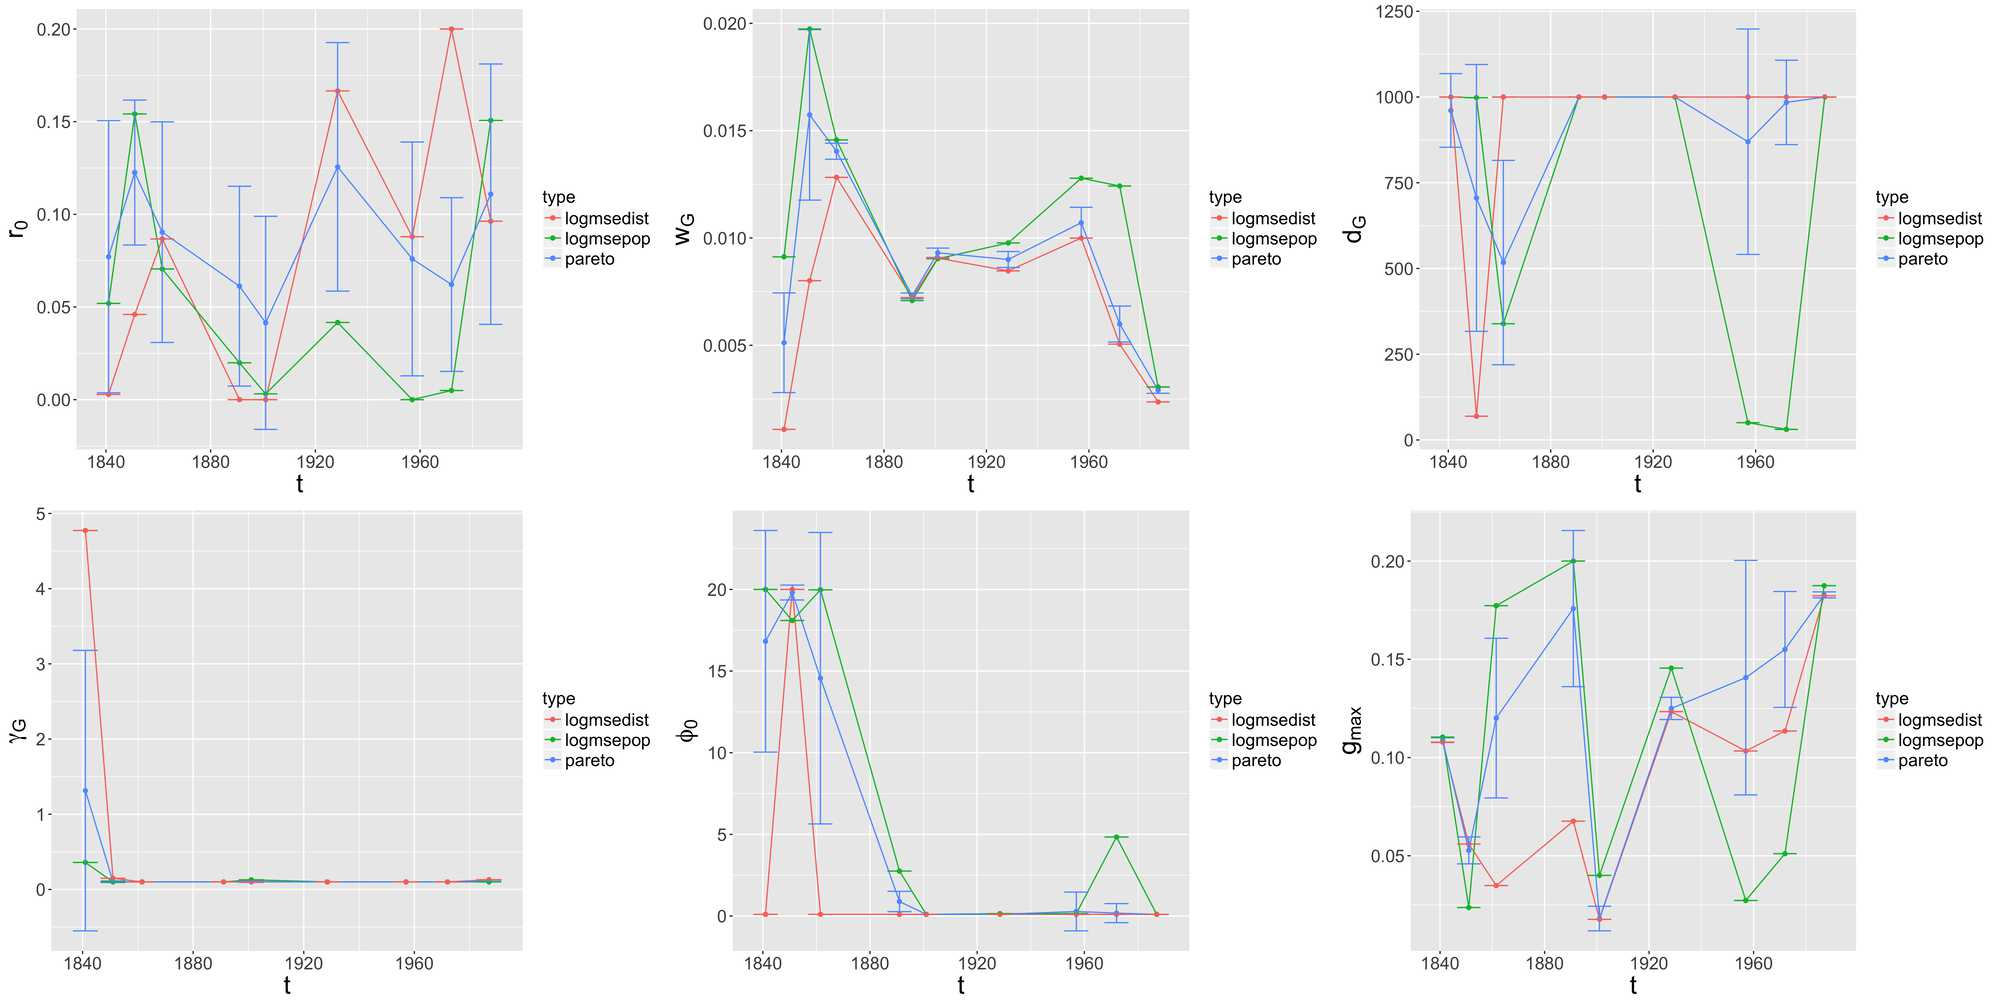
\includegraphics[width=\linewidth]{Figures/Final/6-2-3-fig-macrocoevol-parameters.jpg}
	\caption[Evolution of optimal parameters][Evolution des paramètres optimaux]{\label{fig:macrocoevol:parameters}}{\textbf{Evolution temporelle des paramètres optimaux.} Dans l'ordre de gauche à droite et de haut en bas, valeurs des paramètres $(w_G,d_G,\gamma_G,\gamma_s,\phi_0,g_{max})$, respectivement pour l'ensemble du front de Pareto (bleu), pour le point optimal au sens de la distance (rouge) et pour le point optimal au sens de la population (vert).\comment[FL]{()}\label{fig:macrocoevol:parameters}}
\end{figure}
%%%%%%%%%%%%%%%%%%%








\subsubsection{Physical network}{Modèle avec réseau physique}


Nous esquissons à présent les contours d'une spécification du modèle avec réseau physique, qui correspondrait en un sens à un modèle hybride combinant plusieurs échelles comme nous l'avons déjà argumenté\comment[FL]{ce netait pas ressorti clairement pour moi}. L'idée d'une telle spécification serait d'une part d'étudier l'écart de trajectoire par rapport au réseau abstrait, c'est à dire quantifier l'importance des économies d'échelles (liées aux tronçons communs) et de la congestion, ainsi que les possibles compromis à effectuer liés à la spatialisation du réseau, et d'autre part d'étudier dans quelle mesure il est possible de reproduire des réseaux réalistes en comparaison à des modèles autonomes de croissance de réseau par exemple. Ces questions sont traitées à une autre échelle et pour d'autre spécifications ontologiques au chapitre~\ref{ch:mesocoevolution}. 


Le réseau physique que nous implémentons cherche à satisfaire un critère gourmand\comment[FL]{?} de gain de temps local. Plus précisément, on suppose un auto-renforcement à la manière de~\cite{tero2010rules}. Une specification analogue à celle utilisée précédemment suppose une croissance pour chaque lien, donnée par :

\[
d(t+1) = d(t)\cdot \left(1 + g_{max} \cdot \left[\frac{\phi}{\max \phi}\right]^{\gamma_s}\right)
\]

\comment[AB]{expliciter l'autorenforcement ici}

la specification par seuil ne permettant pas une bonne convergence dans le temps.

\comment[FL]{repartition des pop pas differentes ?}

Nous générons un réseau initial aléatoire, en perturbant la position des sommets d'une grille dont une proportion fixée de liens a été supprimée (40\%) et en y reliant les villes au plus court. Les liens ont tous même impédance, puis celle-ci évolue selon l'équation ci-dessus. Un exemple de configuration obtenue par cette spécification est donné en Fig.~\ref{fig:macrocoevolution:slimemould}. Les bonnes propriétés de convergence suggèrent les potentialités offertes par cette spécification\comment[AB]{visuelles uniquement ?}, dont l'exploration systématique est hors de notre portée ici.


%%%%%%%%%%%%%%%%%%%%%%
\begin{figure}
	%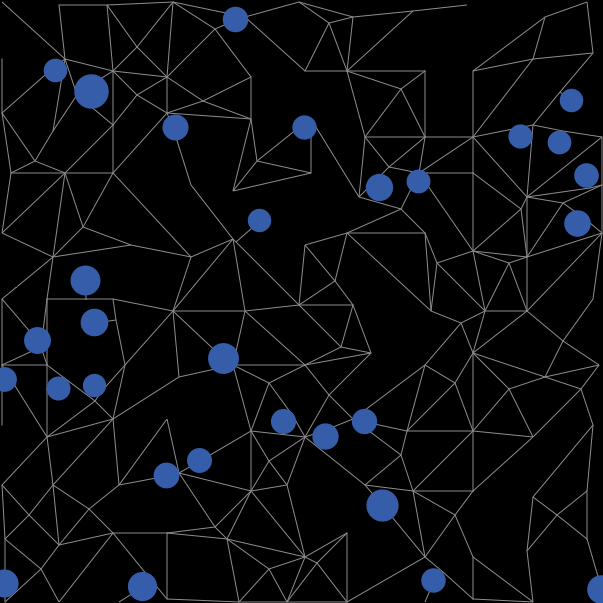
\includegraphics[width=0.45\linewidth]{Figures/MacroCoEvol/example_slimemould_1_t0}
	%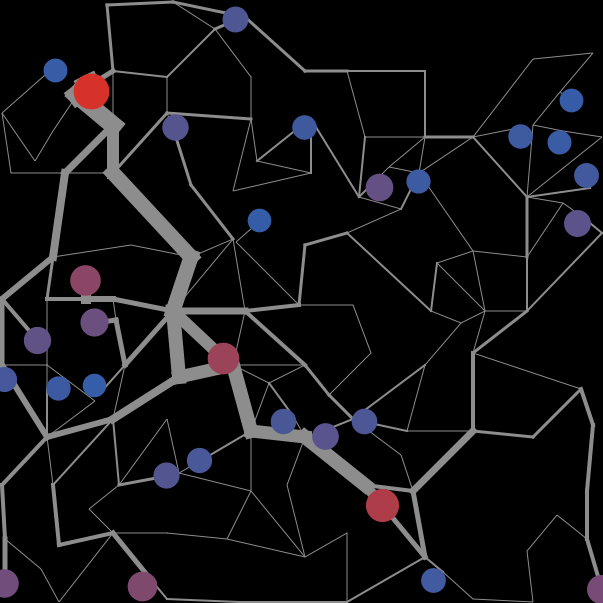
\includegraphics[width=0.45\linewidth]{Figures/MacroCoEvol/example_slimemould_1_tf}
	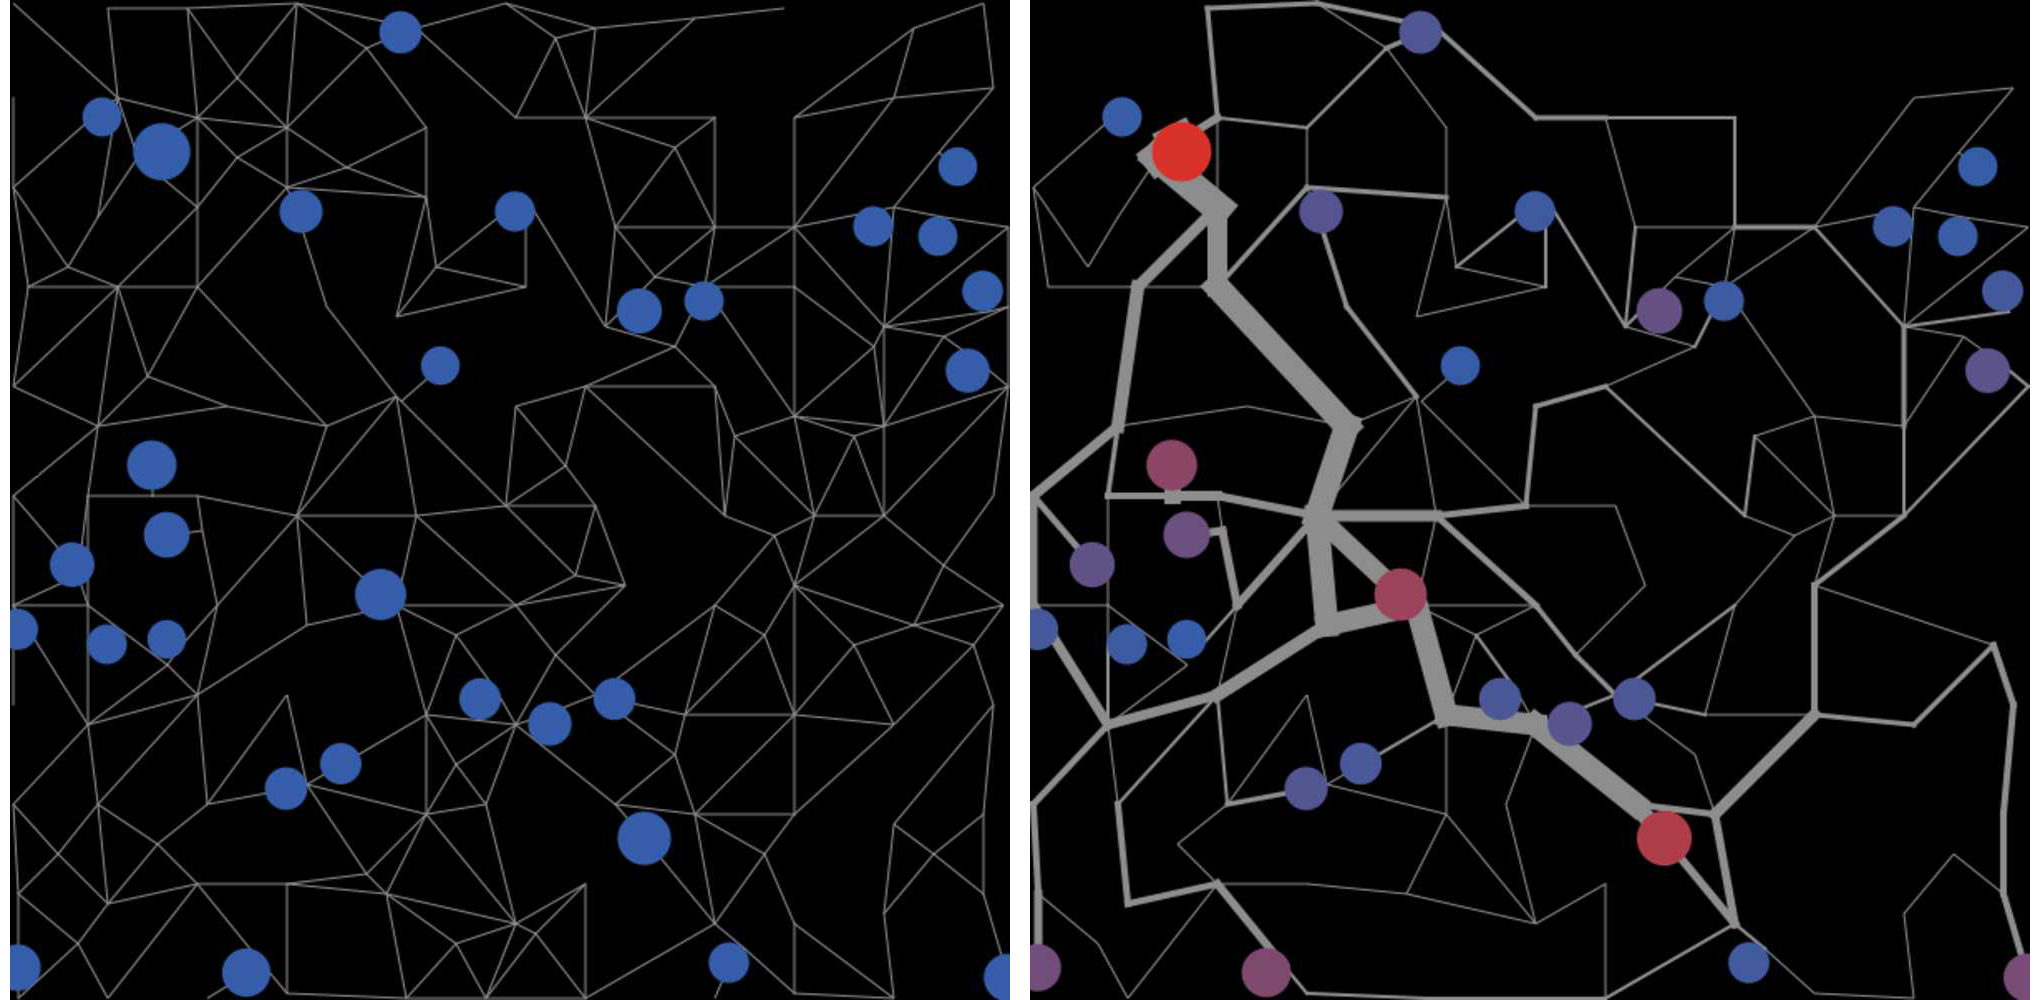
\includegraphics[width=\linewidth]{Figures/Final/6-2-3-fig-macrocoevol-slimemould}
	\caption[][Example de réseau auto-renforçant]{}{\textbf{Example de configuration obtenue avec réseau auto-renforçant.} \textit{(Gauche)} Configuration initiale aléatoire, capacités égales ; \textit{(Droite)} Configuration finale obtenue après 100 itérations.\label{fig:macrocoevolution:slimemould}}
\end{figure}
%%%%%%%%%%%%%%%%%%%%%%


%%%%%%%%%%%%%%%%%
%% ON HOLD


%\begin{enumerate}
%\item le modèle produit-il des formes de réseau crédibles dans le cas du réseau physique ?
%\item éventuellement si les correlations temporelles sont calculées sur les vrais données, le modèle peut-il être calibré au second ordre (sur les correlations/causalités) ?
%\end{enumerate}


%\comment{\cite{mimeur:tel-01451164} la thèse de Mimeur est un pont intéressant entre géographie et approches éco de Levinson (modèle de croissance type slime mould ?). plus fait des stats spatiales pour lier croissance pop et accessibilité : checker si même résulats quand fera spatio-temp causalities sur réseau ferré et autoroutier et croissance pop. remarque : trucs bizzares, essaie d'expliquer pour petites villes, mais pas approprié, pb du choix de l'échelle, de ce qui est du bruit et du signal - semble tout mélanger : importance du preprocessing et traitement du signal (cf correlations des taux de croissance). Tester effets fixes régions/départements ? fait GWR finalement ?}




\subsubsection{Perspectives}{Perspectives}



\paragraph{Particular trajectories}{Trajectoires Particulières}


\bpar{
The role of medium-sized cities on the trajectories of the system can also be examined with the model.
}{
L'étude de trajectoires particulières au sein du système de villes peut permettre de répondre à des questions thématiques spécifiques : par exemple, l'influence des villes moyennes sur la trajectoire globale du système, ou les déterminants d'une plus ou moins bonne ``réussite'' pour ce type de profil. Dans le cas de l'application à un système réel, la cartographie des déviations au modèle dans le temps peut suggérer des particularités régionales.\comment[FL]{justement quels fait stylises a reproduire ?}
}




\paragraph{Comparison of Urban Systems}{Comparaison de systèmes urbains}


\bpar{
Finally, a comparison between the urban systems in different geographical and political contexts and at different scales should unveil implications of planning on the interactions between networks and cities, for example by comparing the rather bottom-up growth of the French railway network to the top-down state-planned French highway and Chinese HSR networks.
}{
On s'attend finalement également à pouvoir par l'intermédiaire de ce modèle comparer des systèmes urbains dans des contextes géographiques et politiques différents, ainsi qu'à différentes échelles. Cela devrait permettre de révéler les implications des actions de planification sur les interactions entre réseaux et territoires. Par exemple, le réseau ferre français a émergé de manière relativement auto-organisée (de par les multiples opérateurs)\comment[FL]{c'est faux}[a reformuler - multi-acteurs (// HSR Chinois)], tandis que les autoroutes ont été fortement planifiées, à l'image du réseau ferré à grande vitesse Chinois, pour lequel un développement précis pourrait être envisagé.
}





\stars





